\documentclass[supercite]{Experimental_Report}

\title{~~~~~~数据结构实验~~~~~~}
\author{崔昊阳}
\school{计算机科学与技术学院}
\classnum{CS2104}
\stunum{U202115415}
\instructor{袁凌}
\date{2022年4月22日}

\usepackage{algorithm, multirow}
\usepackage{algpseudocode}
\usepackage{amsmath}
\usepackage{amsthm}
\usepackage{framed}
\usepackage{mathtools}
\usepackage{subcaption}
\usepackage{xltxtra} %提供了针对XeTeX的改进并且加入了XeTeX的LOGO, 自动调用xunicode宏包(提供Unicode字符宏)
\usepackage{bm}
\usepackage{tikz}
\usepackage{tikzscale}
\usepackage{pgfplots}
%\usepackage{enumerate}
%代码
\usepackage{caption}
% \usepackage[dvipsnames]{xcolor}  % 更全的色系
\usepackage{listings}  % 排代码用的宏包
\lstset{
    language = C,
    backgroundcolor = \color{white},    % 背景色
    basicstyle = \small\ttfamily,           % 基本样式 + 小号字体
    rulesepcolor= \color{gray},             % 代码块边框颜色
    breaklines = true,                  % 代码过长则换行
    numbers = left,                     % 行号在左侧显示
    numberstyle = \small,               % 行号字体
    keywordstyle = \color{blue}\bfseries,      % 关键字颜色
    commentstyle =\color{green},        % 注释颜色
    stringstyle = \color{red},          % 字符串颜色
    frame = shadowbox,                  % 用(带影子效果)方框框住代码块
    showspaces = false,                 % 不显示空格
    columns = fixed,                    % 字间距固定
    %escapeinside={<@}{@>}              % 特殊自定分隔符:<@可以自己加颜色@>
    morekeywords = {as},                % 自加新的关键字(必须前后都是空格)
    deletendkeywords = {compile}        % 删除内定关键字;删除错误标记的关键字用deletekeywords删!
}

\pgfplotsset{compat=1.16}

\newcommand{\cfig}[3]{
  \begin{figure}[htb]
    \centering
    \includegraphics[width=#2\textwidth]{images/#1.tikz}
    \caption{#3}
    \label{fig:#1}
  \end{figure}
}

\newcommand{\sfig}[3]{
  \begin{subfigure}[b]{#2\textwidth}
    \includegraphics[width=\textwidth]{images/#1.tikz}
    \caption{#3}
    \label{fig:#1}
  \end{subfigure}
}

\newcommand{\xfig}[3]{
  \begin{figure}[htb]
    \centering
    #3
    \caption{#2}
    \label{fig:#1}
  \end{figure}
}

\newcommand{\rfig}[1]{\autoref{fig:#1}}
\newcommand{\ralg}[1]{\autoref{alg:#1}}
\newcommand{\rthm}[1]{\autoref{thm:#1}}
\newcommand{\rlem}[1]{\autoref{lem:#1}}
\newcommand{\reqn}[1]{\autoref{eqn:#1}}
\newcommand{\rtbl}[1]{\autoref{tbl:#1}}

\algnewcommand\Null{\textsc{null }}
\algnewcommand\algorithmicinput{\textbf{Input:}}
\algnewcommand\Input{\item[\algorithmicinput]}
\algnewcommand\algorithmicoutput{\textbf{Output:}}
\algnewcommand\Output{\item[\algorithmicoutput]}
\algnewcommand\algorithmicbreak{\textbf{break}}
\algnewcommand\Break{\algorithmicbreak}
\algnewcommand\algorithmiccontinue{\textbf{continue}}
\algnewcommand\Continue{\algorithmiccontinue}
\algnewcommand{\LeftCom}[1]{\State $\triangleright$ #1}

\newtheorem{thm}{定理}[section]
\newtheorem{lem}{引理}[section]

\colorlet{shadecolor}{black!15}

\theoremstyle{definition}
\newtheorem{alg}{算法}[section]

\def\thmautorefname~#1\null{定理~#1~\null}
\def\lemautorefname~#1\null{引理~#1~\null}
\def\algautorefname~#1\null{算法~#1~\null}

\begin{document}

\maketitle


\clearpage

\pagenumbering{Roman}

\tableofcontents[level=2]

\clearpage

\pagenumbering{arabic}

\section{基于链式存储结构的线性表实现}


\subsection{问题描述}

本实验实现了线性表的链式存储,实现了线性表的初始化、销毁、清空等13种基本功能和全部的5种附加功能,还实现了链式的线性表管理。

\subsection{系统设计}

本系统的整体演示系统由功能选择模块、线性表管理模块和功能评测模块组成。
其中,功能选择模块把所有功能打印在屏幕上供使用者选择。
使用者选择相应功能后,线性表管理模块会询问使用者是否存储一些线性表,
使用者可以根据需要按提示进行存储或选择跳过。
在线性表存储结束(或因使用者选择不存储而跳过)后即进入功能评测模块。
使用者可以在3种测试模式间自由选择(部分功能由于各种原因可能缺少一些测评模式),
这三种测试模式分别是:
\begin{enumerate}
\renewcommand{\labelenumi}{\theenumi)}
	\item 自动测试:系统从数据构造器中获取随机数据进行测试,并打印测试报告。输入的数据会存放在testi.txt文件中,部分功能可以查看输出的数据,输出的数据存放在resulti.txt文件中。
	\item 手动输入数据:系统使用由使用者输入的数据进行测试。
	\item 从已有线性表中选择:系统从已有的线性表中获取数据进行测试。
\end{enumerate}

本系统的数据结构有两种:链式线性表和链式线性表的管理表。其具体定义如下。

\begin{lstlisting}[title = 定义,frame=none]
typedef struct LNode  //单链表(链式结构)结点的定义
{
     ElemType data;
     struct LNode *next;
}LNode,*LinkList;
typedef struct LinkLists  //线性表的管理表结点的定义 
{
 	char name[20];//名字。 
 	LinkList heads;//链表的头节点。 
 	struct LinkLists*next;
}LinkLists;
\end{lstlisting}
\subsection{系统实现}

\begin{enumerate}
	\item 初始化线性表\\
	如果线性表不存在,则创建头结点并使头结点的next指针指向NULL,返回成功。
	否则返回不可行。
	\item 销毁线性表\\
	如果线性表存在,遍历线性表并依次释放结点的空间,返回成功,否则返回不可行。
	\item 清空线性表\\
	如果线性表存在,清除它的所有结点,返回成功,否则返回不可行。
	\item 判定线性表是否为空\\
	如果线性表不存在,返回不可行。如果头结点的next指向NULL,返回True,
	否则返回False。
	\item 求线性表的长度\\
	如果线性表不存在,返回不可行。否则遍历线性表,返回结点的数目。
	\item 获取元素\\
	如果线性表不存在,返回不可行。如果索引不大于0,返回索引越界错误。
	否则遍历线性表查找位置,如果遍历完成依然未找到位置,
	返回索引越界错误,否则返回对应位置的元素。
	\item 翻转线性表\\
	如果线性表不存在,返回不可行。否则遍历链表并把每个指针反向以实现翻转,返回成功。时间复杂度O(n)。
	\begin{figure}[htb]
		\begin{center}
			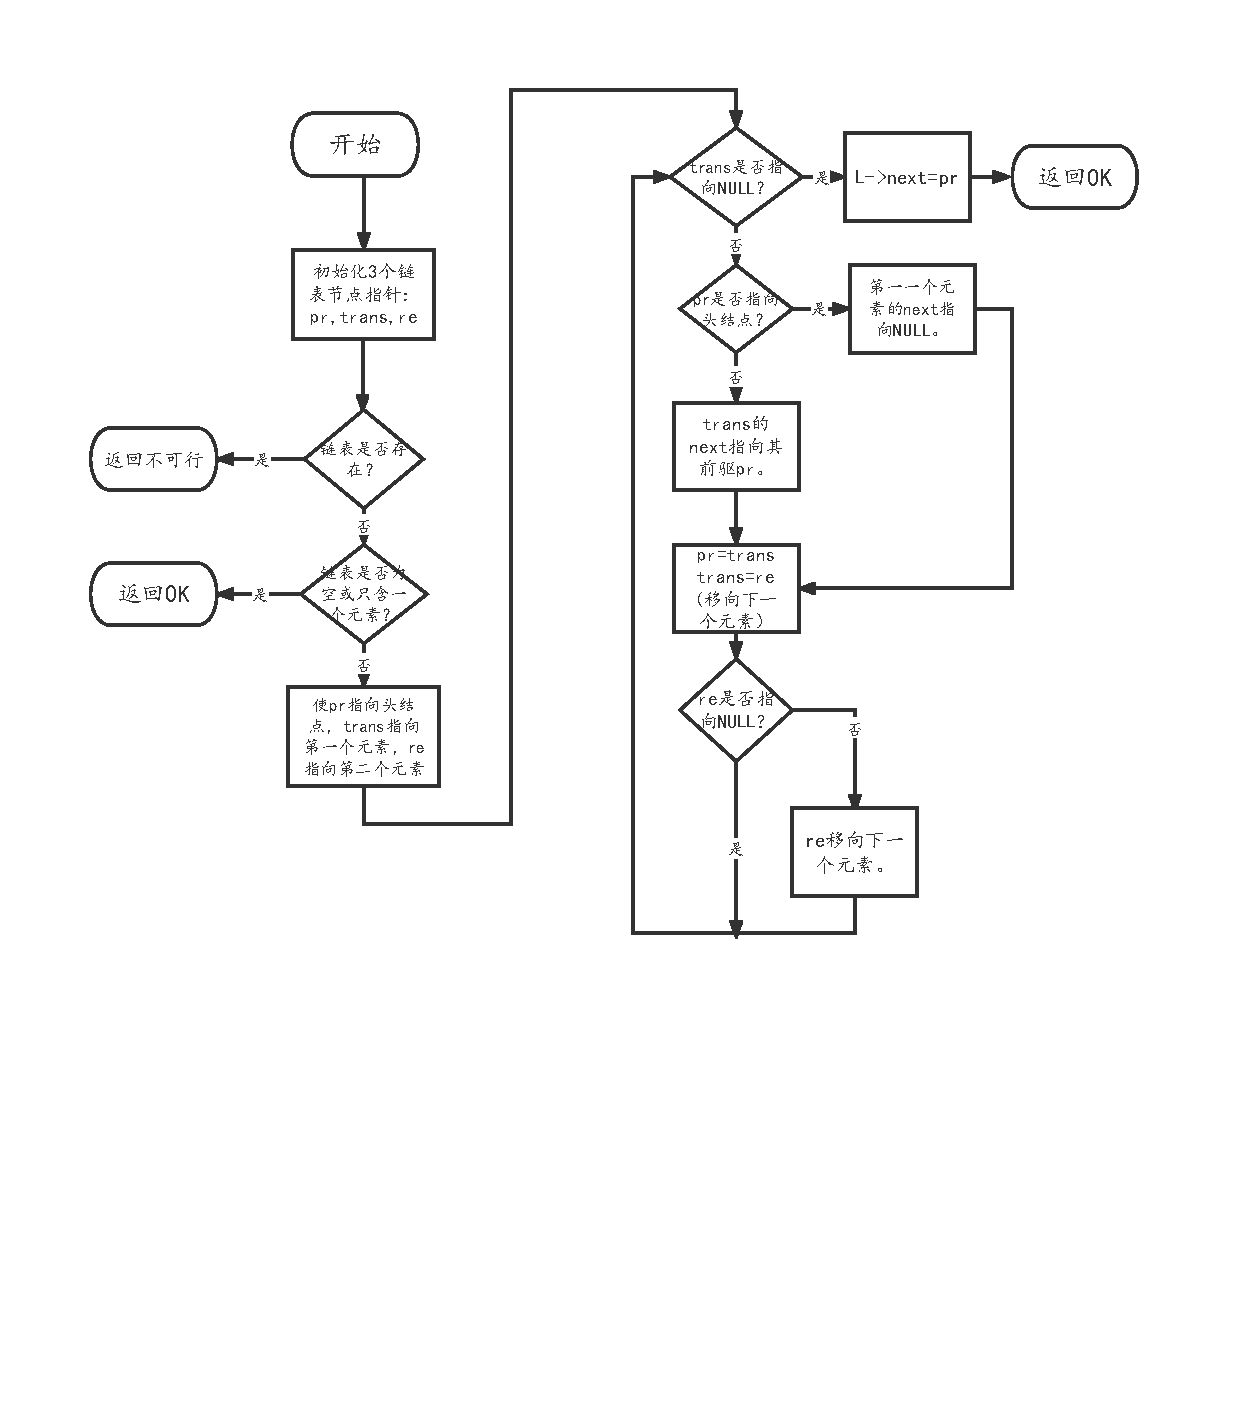
\includegraphics[scale=0.60]{images/数据结构-链表-流程图.pdf}
			\caption{翻转线性表}
			\label{fig1-1}
		\end{center}
	\end{figure}
	\newpage
	\item 排序线性表\\
	如果线性表不存在,返回不可行。采用归并排序进行链表的排序,首先递归地从链表的中间节点(以快慢指针算法寻找)拆分链表到单一节点,
	之后进行合并有序链表的操作。所有操作结束后即得到有序线性表。时间复杂度O(n)。
	\item 查找元素\\
	如果线性表不存在,返回不可行。遍历线性表,记录遍历到的位置,如果遍历到的节点元素是要查找的位置,返回这个位置。
	如果遍历完成后依然未找到,返回不存在。
	\item 获取前驱元素\\
	如果线性表不存在,返回不可行。从第一个元素开始遍历,如果遍历到的节点元素的next是要查找的元素,返回next所指元素。
	如果遍历完成后依然未找到,返回不存在。
	\item  获取后继元素\\
	如果线性表不存在,返回不可行。遍历线性表如果遍历到的节点元素是要查找的元素且元素的next存在,返回next所指元素。
	否则返回不存在。如果遍历完成后依然未找到,返回不存在。
	\item 插入元素\\
	如果线性表不存在,返回不可行。首先遍历链表寻找插入位置,如果索引不大于0,返回索引错误,如果遍历完成后依然未找到,返回索引错误。
	否则分配空间并插入节点。
	\item 删除元素\\
	如果线性表不存在,返回不可行。首先遍历链表寻找删除位置,如果索引不大于0,返回索引错误,如果遍历完成后依然未找到,返回索引错误。
	否则删除节点。
	\item 遍历线性表\\
	如果线性表不存在,返回不可行。否则从第一个元素开始依次访问节点元素直到节点的next指向NULL。
	\item 删除倒数第n个元素\\
	如果线性表不存在,返回不可行。否则遍历链表求出表长,根据表长获得倒数第n个元素的索引,
	根据这个索引遍历链表寻找删除位置,如果索引不大于0,返回索引错误,如果遍历完成后依然未找到,返回索引错误。
	否则删除节点。时间复杂度O(n)。
	\item 线性表的文件操作\\
	如果线性表不存在,返回不可行。打开只写文件,遍历线性表并依次写入元素。销毁线性表。接着初始化线性表,
	以只读模式打开刚才保存的文件,依次读入各元素,新建节点并插入线性表,直到读取到EOF。
\end{enumerate}
\subsection{系统测试}
本段我们采用多种方式测试上述各函数。在非自动测试的情况下,线性表输入值取[1,5,4,2,3]。
在自动测试情况下,线性表输入取0个值(但非空表)、10000个值和1000000个值。
	\begin{enumerate}
		\item 多线性表管理\\
		输入[1,5,4,2,3],输出结果如下图:
		\begin{figure}[htb]
			\begin{center}
				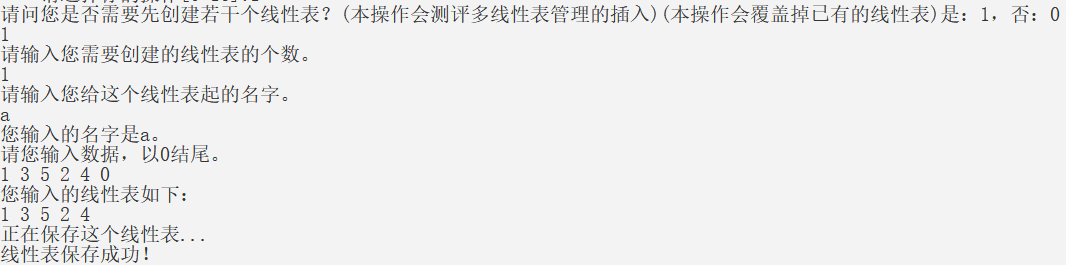
\includegraphics[scale=0.60]{images/链表-多线性表管理.png}
				\caption{链表-多线性表管理测试}
				\label{fig1-2}
			\end{center}
		\end{figure}
		\item 初始化线性表\\
		输入[1,5,4,2,3],输出结果如下图:
		\begin{figure}[htb]
			\begin{center}
				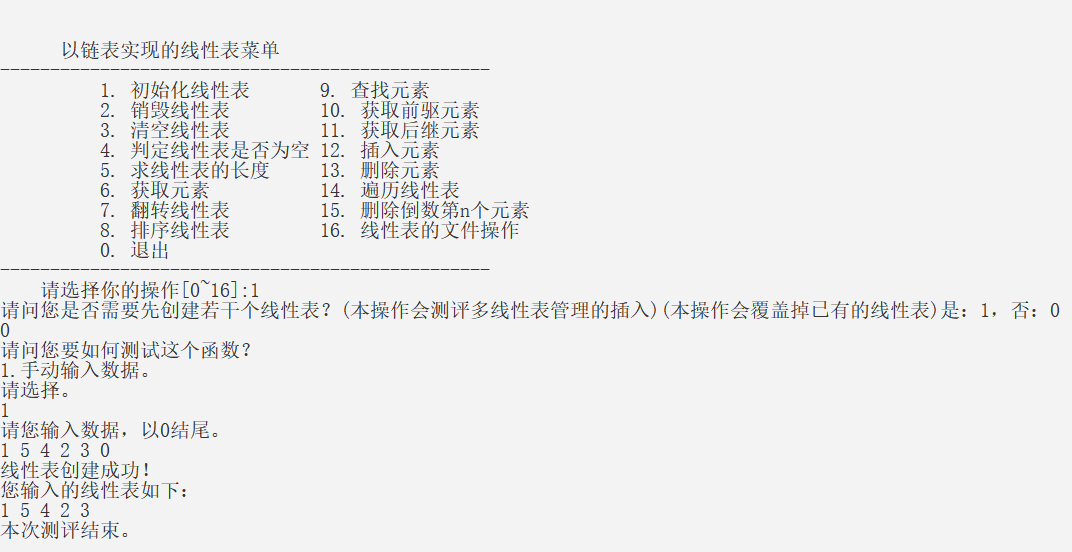
\includegraphics[scale=0.60]{images/链表-初始化.png}
				\caption{链表-初始化测试}
				\label{fig1-3}
			\end{center}
		\end{figure}
		\newpage
		\item 销毁线性表\\
		选择自动测试,输出结果如下图:
		\begin{figure}[htb]
			\begin{center}
				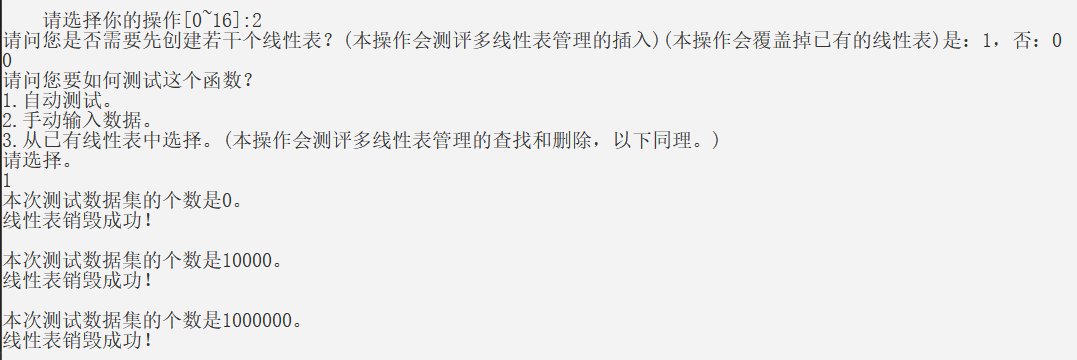
\includegraphics[scale=0.60]{images/链表-销毁.png}
				\caption{链表-销毁测试}
				\label{fig1-4}
			\end{center}
		\end{figure}
		\item 清空线性表\\
		选择自动测试,输出结果如下图:
		\begin{figure}[htb]
			\begin{center}
				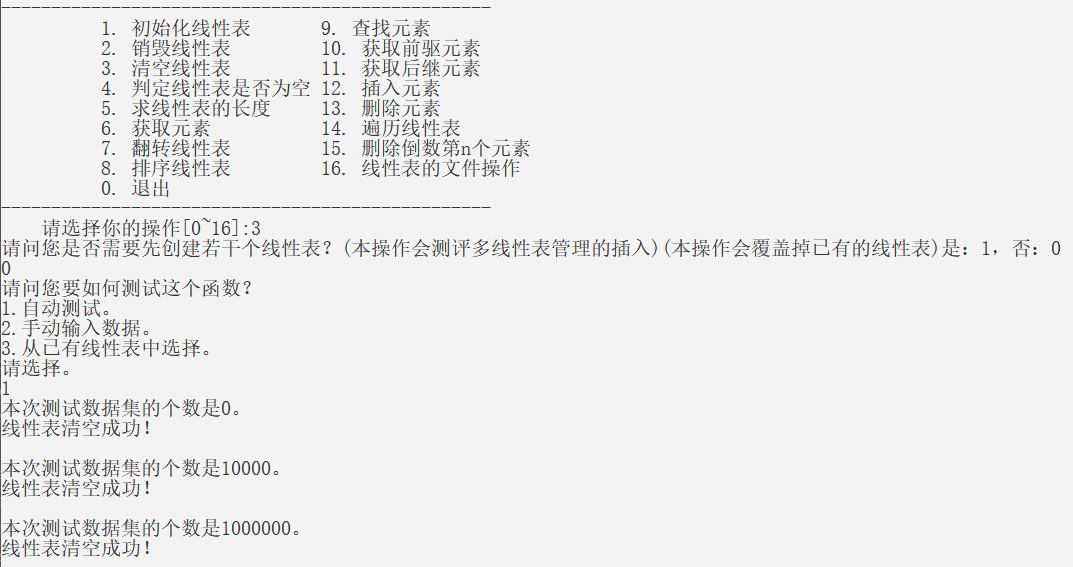
\includegraphics[scale=0.60]{images/链表-清空.png}
				\caption{链表-清空测试}
				\label{fig1-5}
			\end{center}
		\end{figure}
		\newpage
		\item 判定线性表是否为空\\
		选择自动测试,输出结果如下图:
		\begin{figure}[htb]
			\begin{center}
				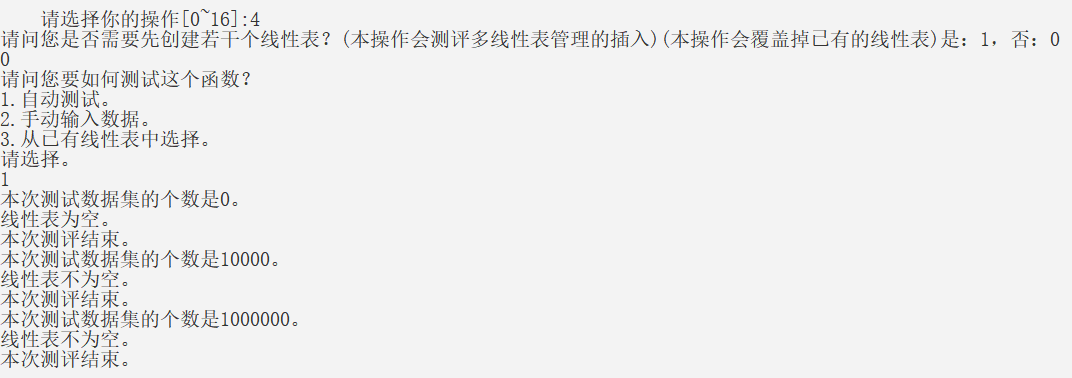
\includegraphics[scale=0.60]{images/链表-判空.png}
				\caption{链表-判空测试}
				\label{fig1-6}
			\end{center}
		\end{figure}
		\item 求线性表的长度\\
		选择自动测试,输出结果如下图:
		\begin{figure}[htb]
			\begin{center}
				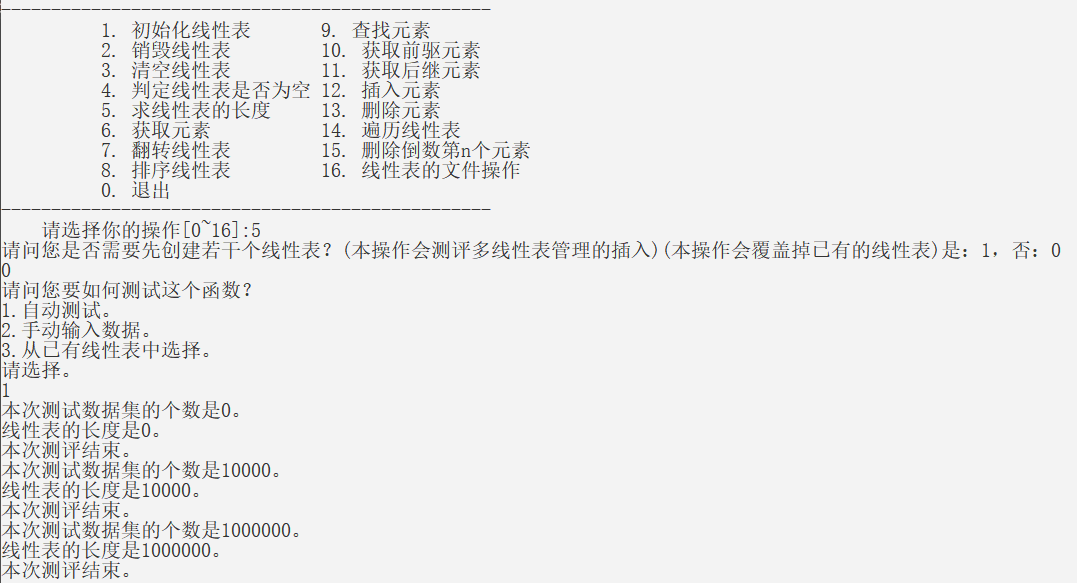
\includegraphics[scale=0.60]{images/链表-求表长.png}
				\caption{链表-求表长测试}
				\label{fig1-7}
			\end{center}
		\end{figure}
		\newpage
		\item 获取元素\\
		输入[1,5,4,2,3],索引2和10,输出结果如下图:
		\begin{figure}[htb]
			\begin{center}
				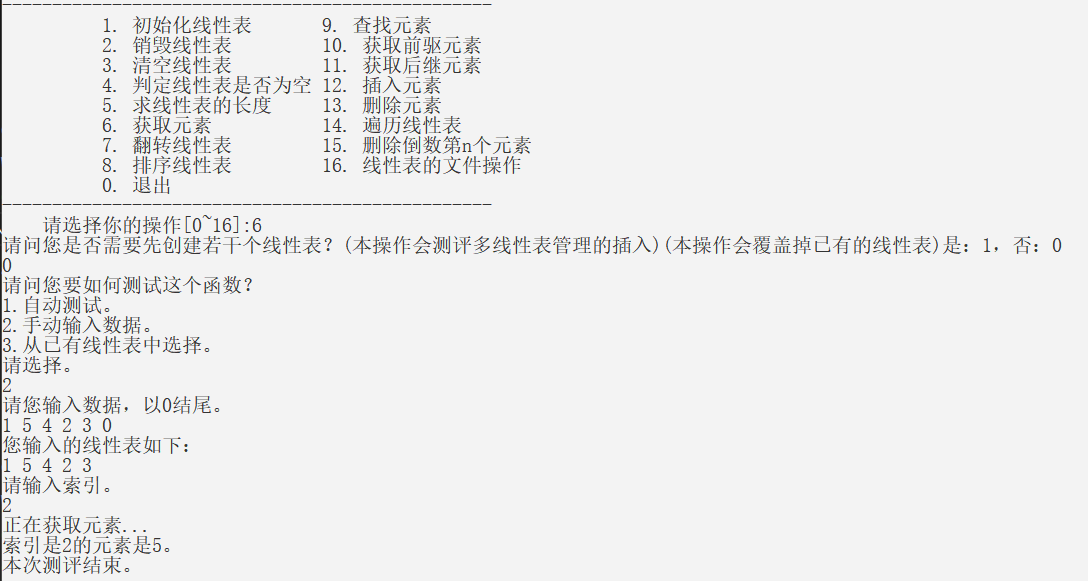
\includegraphics[scale=0.60]{images/链表-获取元素.png}
				\caption{链表-获取元素测试1}
				\label{fig1-8.1}
			\end{center}
		\end{figure}
		\begin{figure}[htb]
			\begin{center}
				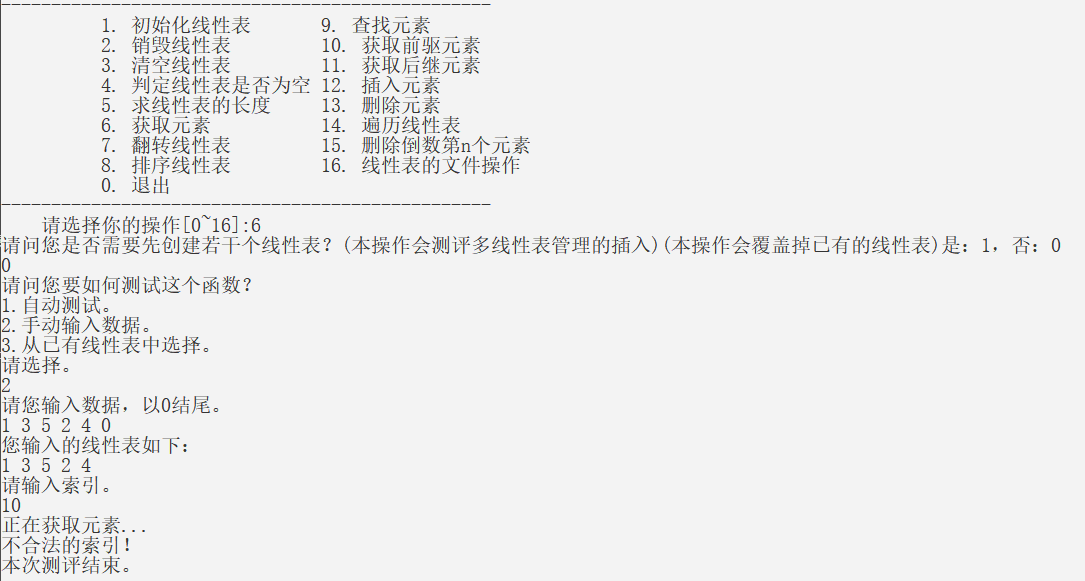
\includegraphics[scale=0.60]{images/链表-获取元素异常.png}
				\caption{链表-获取元素测试2}
				\label{fig1-8.2}
			\end{center}
		\end{figure}
		\newpage
		\item 翻转线性表\\
		输入[1,5,4,2,3],输出结果如下图:
		\begin{figure}[htb]
			\begin{center}
				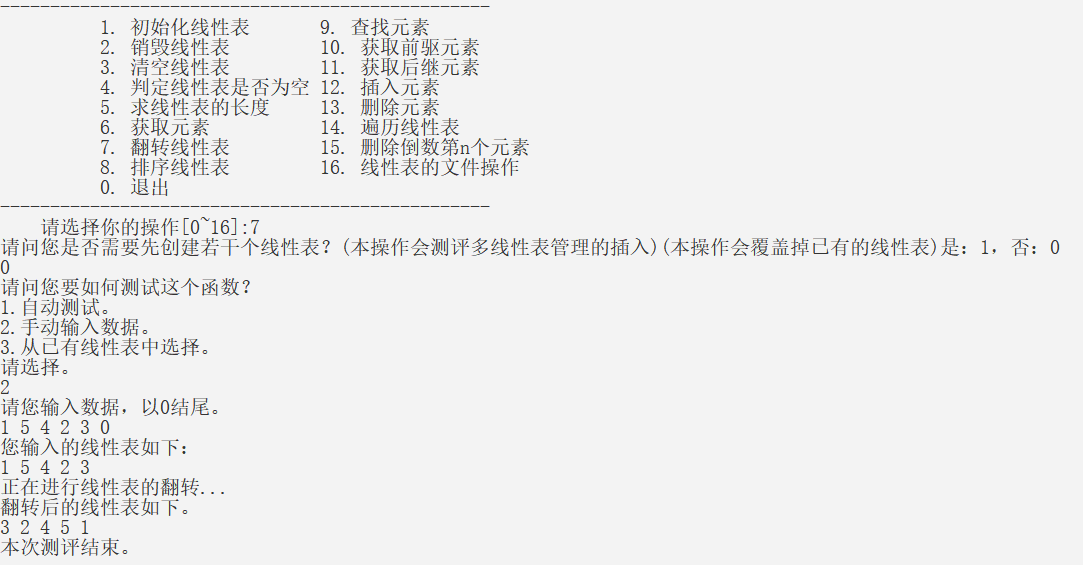
\includegraphics[scale=0.60]{images/链表-翻转链表.png}
				\caption{链表-翻转测试}
				\label{fig1-9}
			\end{center}
		\end{figure}
		\item 排序线性表\\
		输入[1,5,4,2,3],输出结果如下图:
		\begin{figure}[htb]
			\begin{center}
				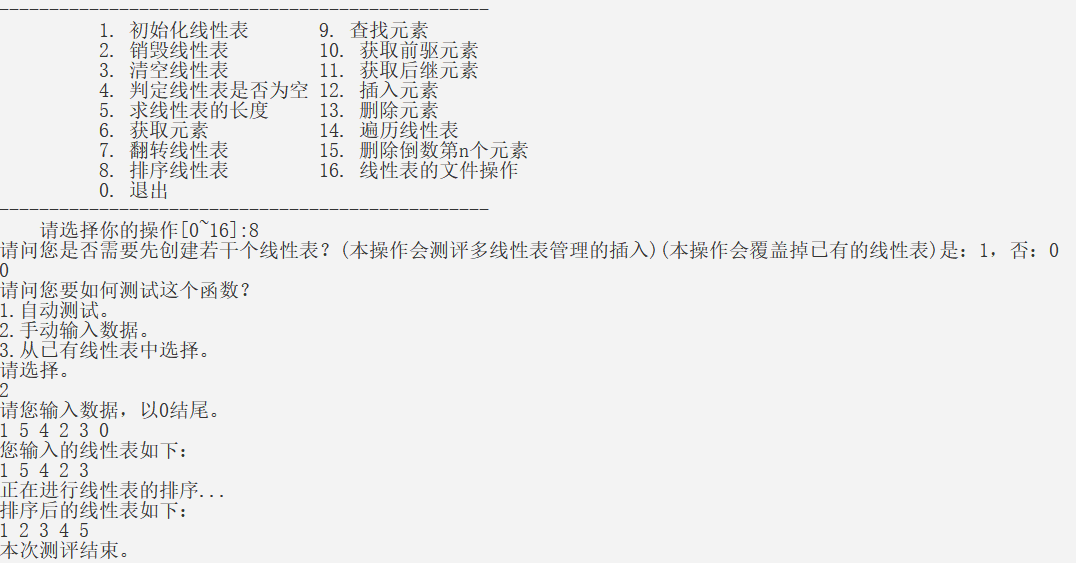
\includegraphics[scale=0.60]{images/链表-排序.png}
				\caption{链表-排序测试}
				\label{fig1-10}
			\end{center}
		\end{figure}
		\newpage
		\item 查找元素\\
		输入[1,5,4,2,3],查找5和10,输出结果如下图:
		\begin{figure}[htb]
			\begin{center}
				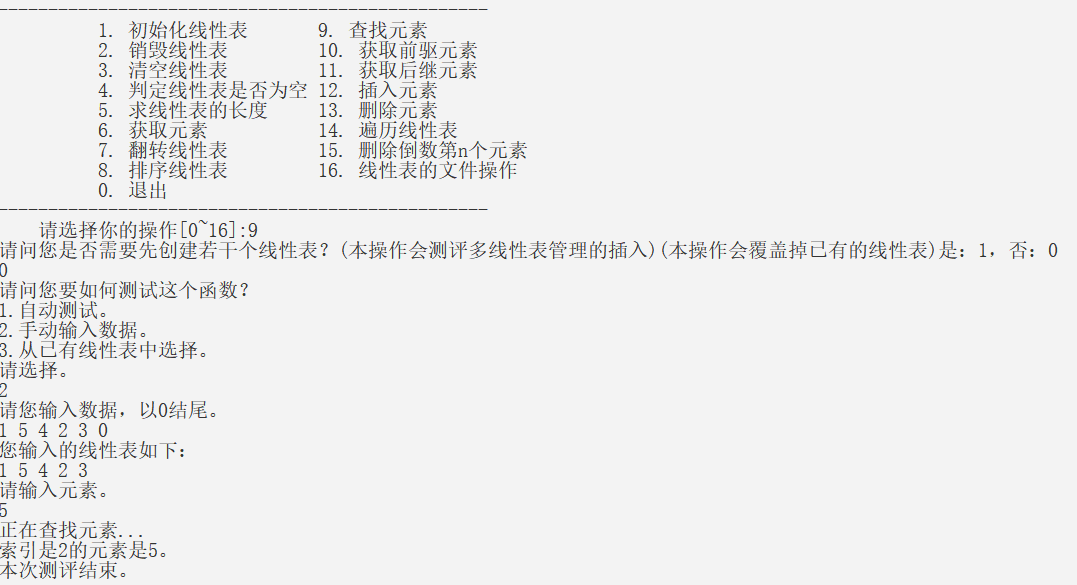
\includegraphics[scale=0.60]{images/链表-查找元素.png}
				\caption{链表-查找元素测试1}
				\label{fig1-11.1}
			\end{center}
		\end{figure}
		\begin{figure}[htb]
			\begin{center}
				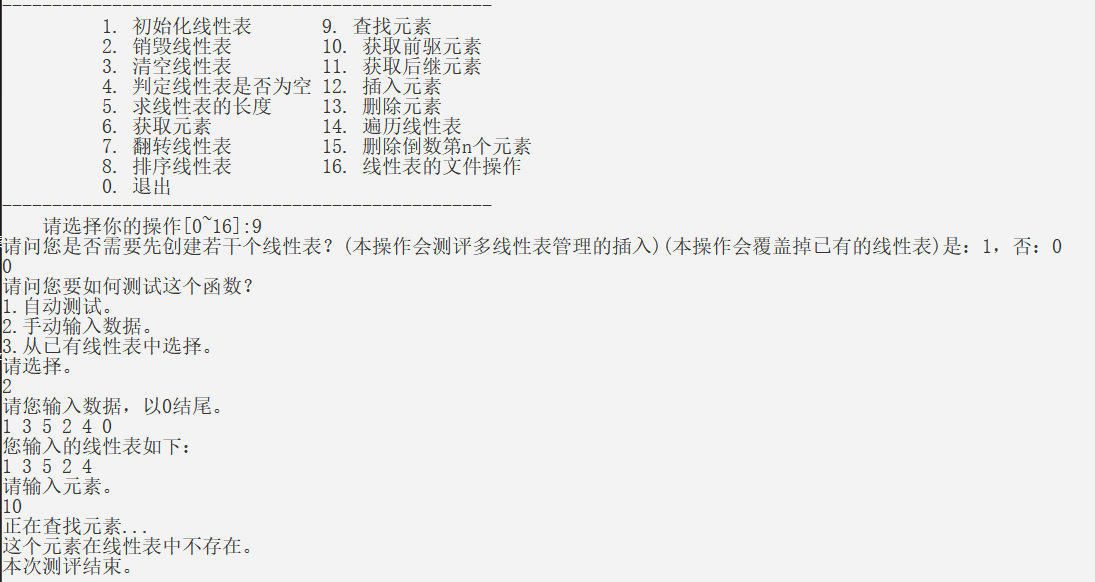
\includegraphics[scale=0.60]{images/链表-查找元素异常.png}
				\caption{链表-查找元素测试2}
				\label{fig1-11.2}
			\end{center}
		\end{figure}
		\newpage
		\item 获取前驱元素\\
		输入[1,5,4,2,3],元素5和1,输出结果如下图:
		\begin{figure}[htb]
			\begin{center}
				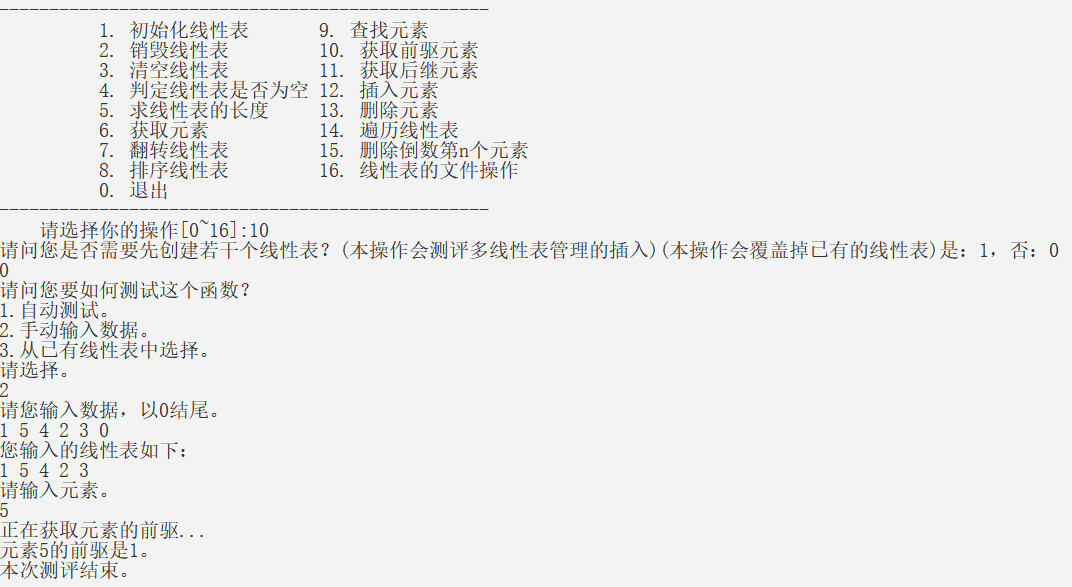
\includegraphics[scale=0.60]{images/链表-获取前驱元素.png}
				\caption{链表-获取前驱元素测试1}
				\label{fig1-12.1}
			\end{center}
		\end{figure}
		\begin{figure}[htb]
			\begin{center}
				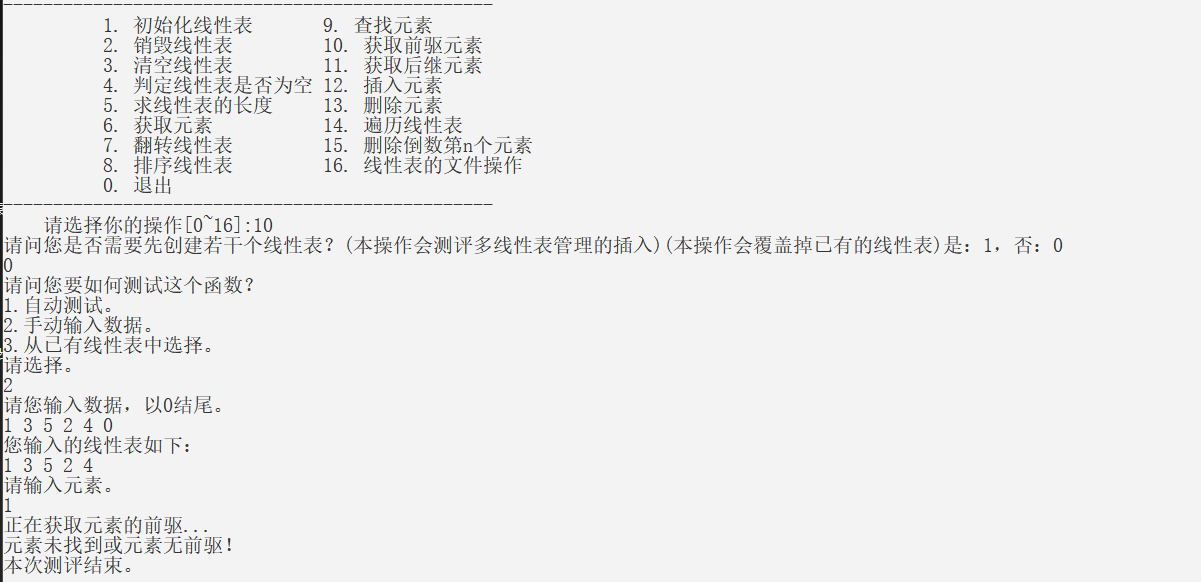
\includegraphics[scale=0.60]{images/链表-获取前驱元素异常.png}
				\caption{链表-获取前驱元素测试2}
				\label{fig1-12.2}
			\end{center}
		\end{figure}
		\newpage
		\item 获取后继元素\\
		输入[1,5,4,2,3],元素5和3,输出结果如下图:
		\begin{figure}[htb]
			\begin{center}
				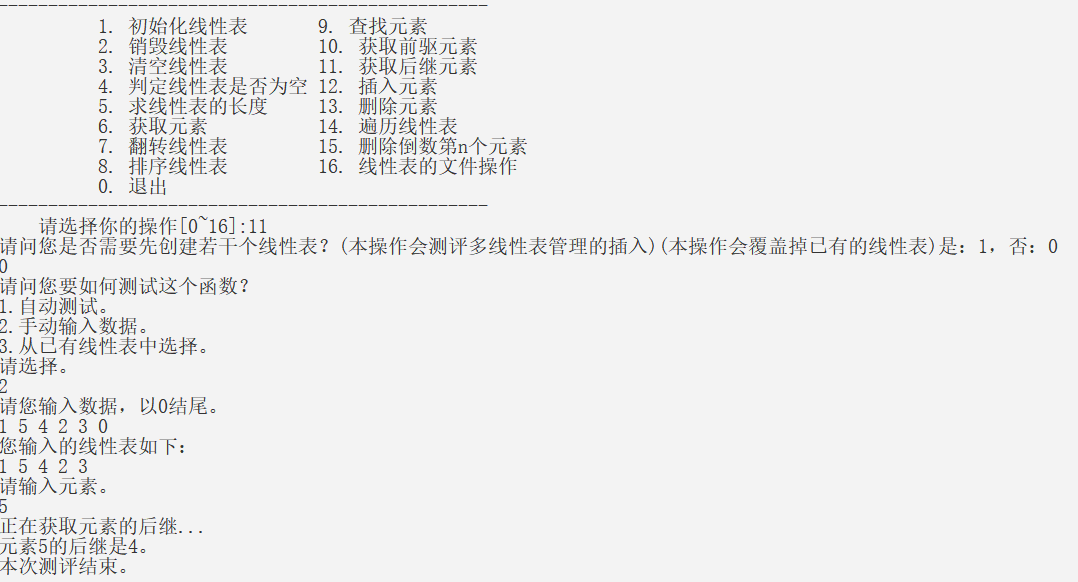
\includegraphics[scale=0.60]{images/链表-获取后继元素.png}
				\caption{链表-获取后继元素测试1}
				\label{fig1-13.1}
			\end{center}
		\end{figure}
		\begin{figure}[htb]
			\begin{center}
				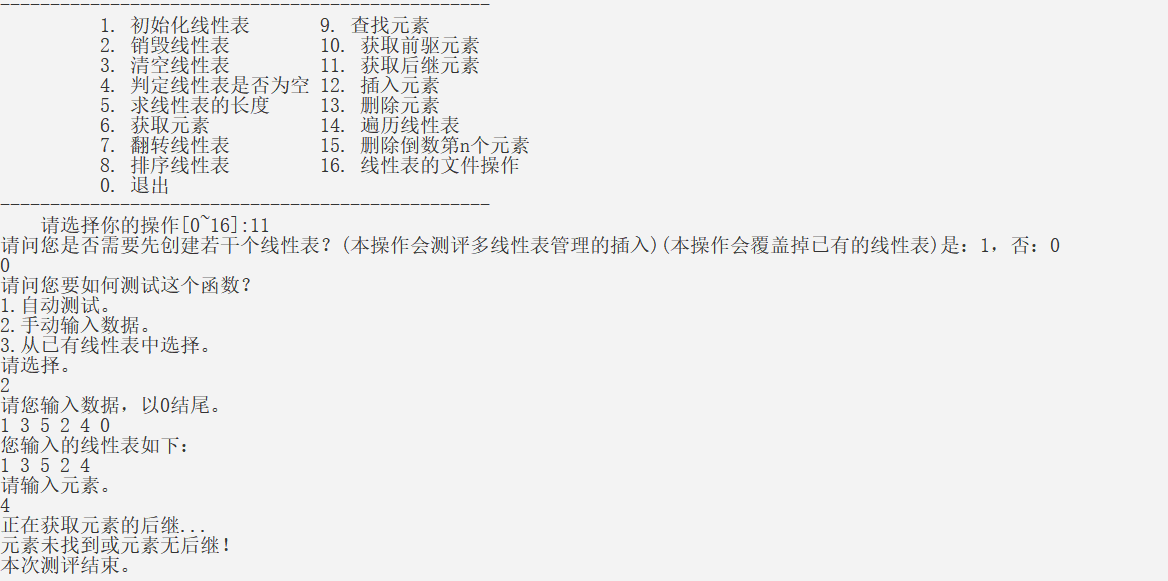
\includegraphics[scale=0.60]{images/链表-获取后继元素异常.png}
				\caption{链表-获取后继元素测试2}
				\label{fig1-13.2}
			\end{center}
		\end{figure}
		\newpage
		\item 插入元素\\
		选择自动测试,输出结果如下图:
		\begin{figure}[htb]
			\begin{center}
				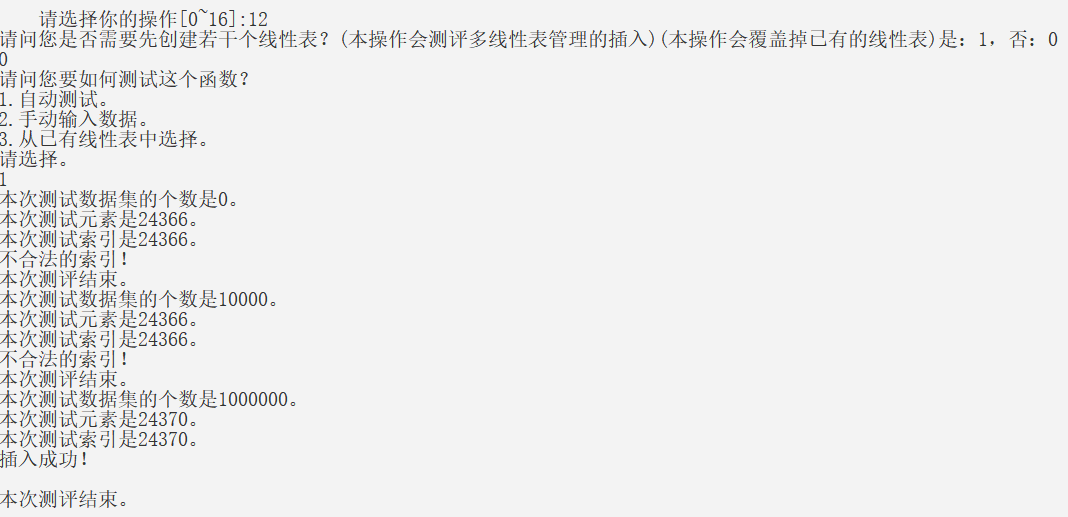
\includegraphics[scale=0.60]{images/链表-插入元素.png}
				\caption{链表-插入元素测试}
				\label{fig1-14}
			\end{center}
		\end{figure}
		\newpage
		\item 删除元素\\
		输入[1,5,4,2,3],删除元素5和10,输出结果如下图:
		\begin{figure}[htb]
			\begin{center}
				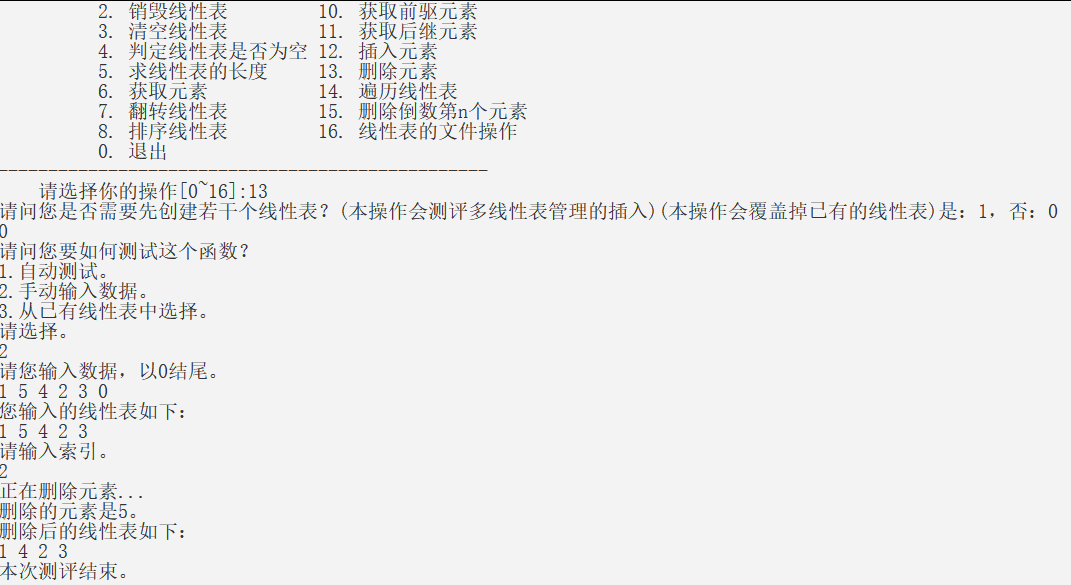
\includegraphics[scale=0.60]{images/链表-删除元素.png}
				\caption{链表-删除元素测试1}
				\label{fig1-15.1}
			\end{center}
		\end{figure}
		\begin{figure}[htb]
			\begin{center}
				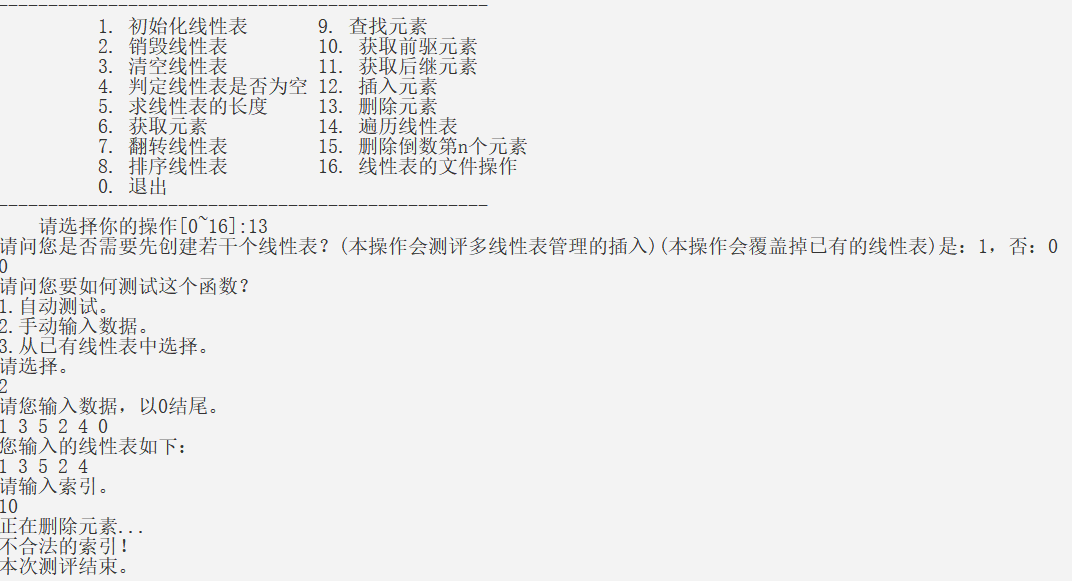
\includegraphics[scale=0.60]{images/链表-删除元素异常.png}
				\caption{链表-删除元素测试2}
				\label{fig1-15.2}
			\end{center}
		\end{figure}
		\newpage
		\item 遍历线性表\\
		输入[1,5,4,2,3],输出结果如下图:
		\begin{figure}[htb]
			\begin{center}
				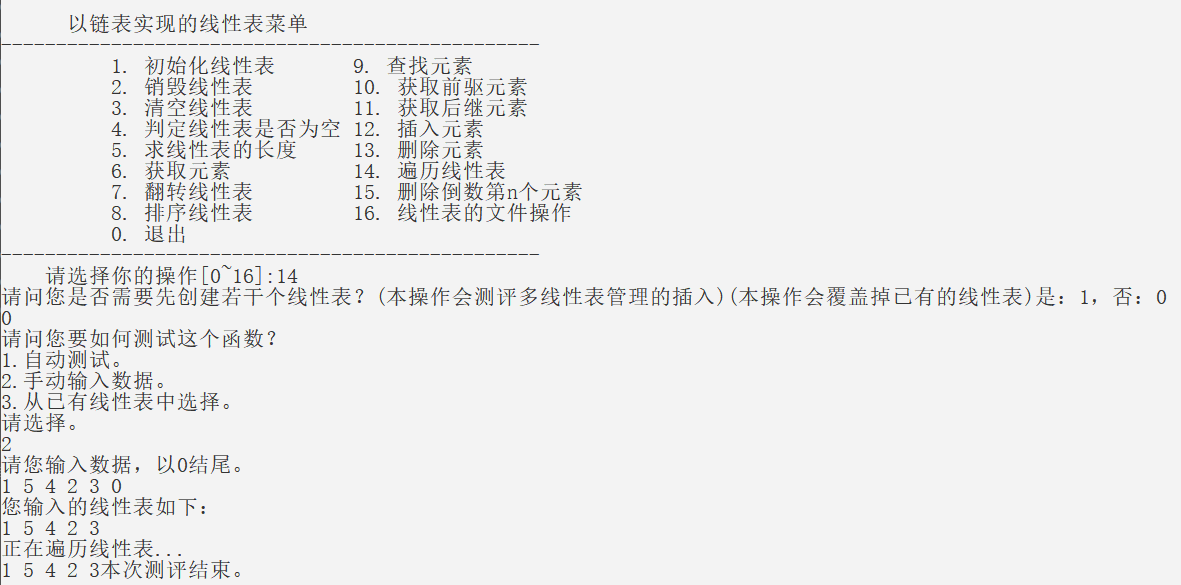
\includegraphics[scale=0.60]{images/链表-遍历.png}
				\caption{链表-遍历测试}
				\label{fig1-16}
			\end{center}
		\end{figure}
		\newpage
		\item 删除倒数第n个元素\\
		输入[1,5,4,2,3],删除倒数第2个和第10个元素,输出结果如下图:
		\begin{figure}[htb]
			\begin{center}
				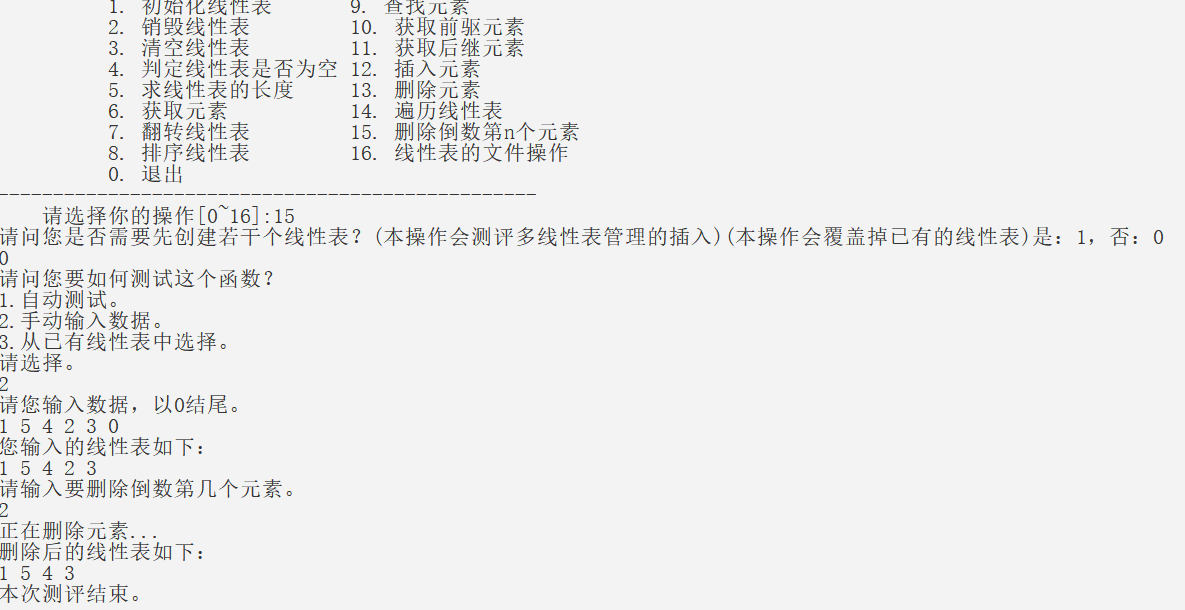
\includegraphics[scale=0.60]{images/链表-删除倒数第n个元素.png}
				\caption{链表-删除倒数第n个元素测试1}
				\label{fig1-17.1}
			\end{center}
		\end{figure}
		\begin{figure}[htb]
			\begin{center}
				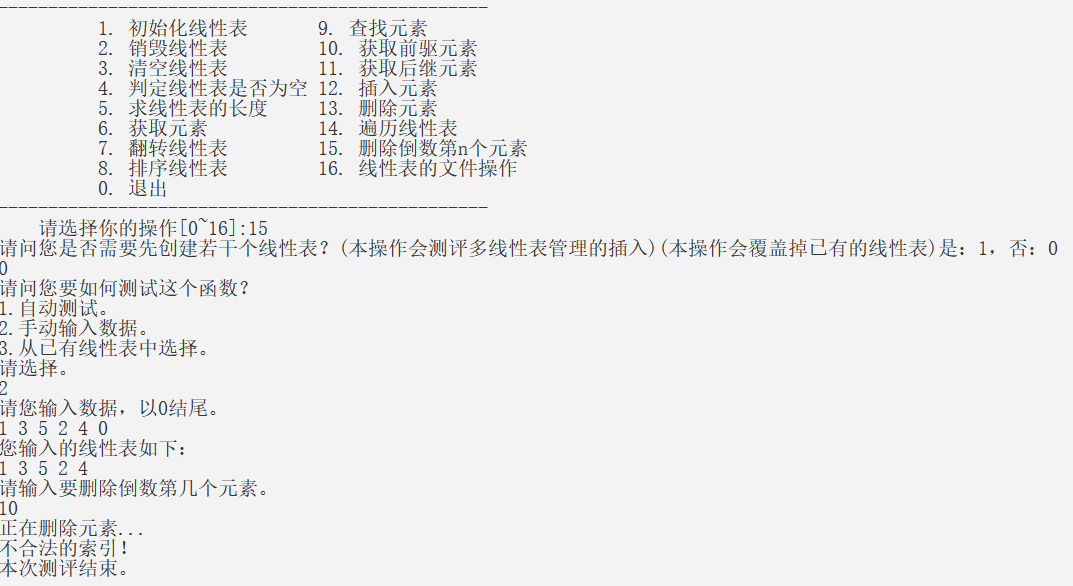
\includegraphics[scale=0.60]{images/链表-删除倒数第n个元素异常.png}
				\caption{链表-删除倒数第n个元素测试2}
				\label{fig1-17.2}
			\end{center}
		\end{figure}
		\newpage
		\item 线性表的文件操作\\
		输入[1,5,4,2,3],输出结果如下图:
		\begin{figure}[htb]
			\begin{center}
				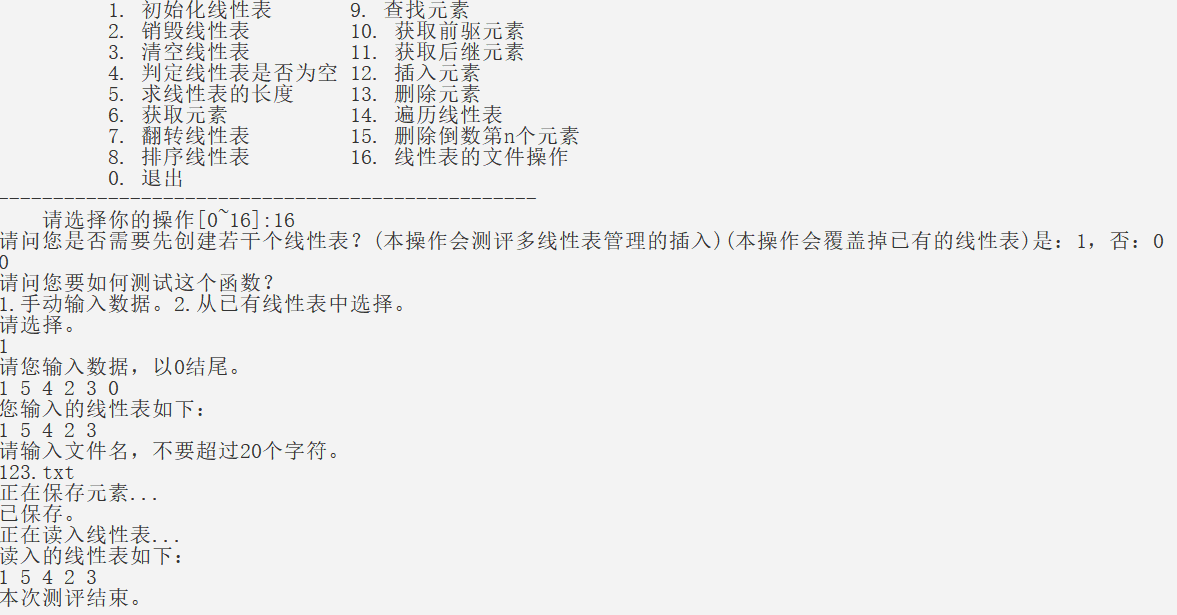
\includegraphics[scale=0.60]{images/链表-文件操作.png}
				\caption{链表-文件操作测试}
				\label{fig1-18.1}
			\end{center}
		\end{figure}
		\begin{figure}[htb]
			\begin{center}
				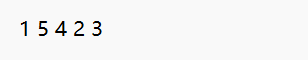
\includegraphics[scale=2.50]{images/链表-文件.png}
				\caption{链表-文件操作测试}
				\label{fig1-18.2}
			\end{center}
		\end{figure}
		\newpage
	\end{enumerate}

\subsection{实验小结}
通过本次实验,我加深了对链式存储的线性表的理解,并掌握了如何运用单链表解决实际问题。
通过本次实验,我学到了:
\begin{enumerate}
	\item 单链表的定义
    \item 单链表的基本操作算法
	\item 链式存储线性表的定义
    \item 链式存储线性表的基本操作算法
    \item 链式存储线性表的管理表的定义
    \item 链式存储线性表的管理表的基本操作算法
    \item 单链表的实际应用
\end{enumerate}
通过本次实验,我认为我还有如下不足之处:
\begin{enumerate}
	\item 对单链表的指针操作不太熟练
    \item 不太明确线性表的实际应用
\end{enumerate}
\newpage

\section{基于二叉链表的二叉树实现}


\subsection{问题描述}

本实验实现了二叉树的二叉链表存储,实现了二叉树的初始化、清空、求二叉树的深度等14种基本功能和全部的5种附加功能,还实现了多二叉树管理。

\subsection{系统设计}

本系统的整体演示系统由功能选择模块、二叉树管理模块和功能评测模块组成。
其中,功能选择模块把所有功能打印在屏幕上供使用者选择。
使用者选择相应功能后,二叉树管理模块会询问使用者是否存储一些二叉树,
使用者可以根据需要按提示进行存储或选择跳过。
在二叉树存储结束(或因使用者选择不存储而跳过)后即进入功能评测模块。
使用者可以在2种测试模式间自由选择(部分功能由于各种原因可能只有一种测评模式),
这两种测试模式分别是:
\begin{enumerate}
	\renewcommand{\labelenumi}{\theenumi)}
		\item 手动输入数据:系统使用由使用者输入的数据进行测试。
		\item 从已有二叉树中选择:系统从已有的二叉树中获取数据进行测试。
	\end{enumerate}
本系统的数据结构有两种:二叉树和二叉树的管理表。其具体定义如下。
\begin{lstlisting}[title = 定义,frame=none]
typedef struct
{
	KeyType  key;
	char others[20];
} TElemType; //二叉树结点类型定义
typedef struct BiTNode//二叉链表结点的定义
{
	TElemType  data;
	struct BiTNode *lchild,*rchild;
} BiTNode, *BiTree;
void visit(BiTree T){printf(" %d,%s",T->data.key,T->data.others);}//遍历visit函数。 
void free0(void*p);
typedef struct//二叉树的管理表的定义。 
{
	BiTree trees[MAX_SIZE];//二叉树指针。 
	char*name[MAX_SIZE];//名字。 
	int len;
	const int listsize=MAX_SIZE;
}BiTrees;		
\end{lstlisting}

\subsection{系统实现}

\begin{enumerate}
	\item 创建二叉树\\
	如果二叉树已存在,返回不可行。调用isrepeat函数检查关键字是否重复,若重复返回错误,否则调用递归函数create。
	递归函数通过definition数组检查输入的结点是否是空结点,若是则返回,否则创建并插入结点,再递归地创建左子树和右子树。
	\item 清空二叉树\\
	如果二叉树不存在,返回不可行。遇到空结点返回,递归地遍历左子树和右子树后释放结点空间。
	\item 求二叉树的深度\\
	遇到空结点返回,否则递归地计算左子树和右子树的深度,都加1后取较大的值的返回。
	\item 查找结点\\
	新建结点指针p指向NULL,然后调用递归函数sol求解,sol若传入的结点是要查找的结点,则把p复制成该结点并返回,遇到空节点也返回,
	否则递归地查找左子树和右子树。最后返回p。
	\item 结点赋值\\
	首先检查关键字是否重复,然后查找结点。如果结点关键字重复或结点未找到,返回错误,
	否则把找到的结点的关键字和名称赋值成用户输入的值。
	\item 获取兄弟结点\\
	首先检查传入的结点是否是指定结点的双亲结点,如果是,返回其兄弟结点。如果结点为空,返回。
	否则递归地查找左子树和右子树。
	\item 插入结点\\
	首先检查关键字是否重复,然后查找结点。如果结点关键字重复或结点未找到,返回错误,
	否则新建结点并按规则进行插入操作。
	\item 删除结点\\
	首先检查关键字是否重复,然后查找双亲结点。如果双亲进度结点未找到且删除的是根结点,直接清空二叉树,否则返回。
	然后递归地删除对应结点左子树和右子树上的所有结点并释放空间。
	\item 先序遍历\\
	首先访问结点,在递归地访问左子树和右子树。
	\item 中序遍历\\
	首先递归地访问左子树,然后访问结点,再递归地访问右子树。
	\item 后序遍历\\
	首先递归地访问左子树和右子树,再访问结点。
	\item 按层遍历\\
	采用广度优先搜索遍历二叉树。首先新建队列并将根结点入队,然后逐个访问队首元素,把队首元素的未入队子结点入队,弹出队首元素,
	直到队列为空。
	\item 翻转二叉树\\
	首先交换传入结点的两个子结点,如果是空结点则返回,然后递归地翻转左子树和右子树。
	\item 最大路径和\\
	遇到空结点返回,否则递归地计算左子树和右子树的最大路径和,取最大的一个的值加上传入顶点的权值后返回。
	\item 最近公共祖先\\
	首先查找结点,如果两个结点中有未找到的,返回错误。然后调用递归函数LCA,LCA中序遍历二叉树,从访问了一个结点开始计数,
	求这时开始到访问到第二个结点时到达的层数最小的结点,这个结点就是最近公共祖先。
	\item 线性表的文件操作\\
	打开只写文件,调用递归函数save,如果传入结点为空,返回。写入传入的二叉树结点,然后递归地写入左子树和右子树。最后清空二叉树。
	接着创建新二叉树,以只读模式打开刚才保存的文件,调用递归函数load,新建结点,读入数据。插入新二叉树,
	然后递归地读取左子树和右子树。
\end{enumerate}
\subsection{系统测试}

本段我们采用多种方式测试上述各函数。手动输入的数据是
1 a 2 b 0 null  0 null 3 c 4 d  0 null  0 null 5 e  0 null  0 null -1 null,我们称其为二叉树A。
\begin{enumerate}
	\item 创建二叉树\\
	输入二叉树A,输出结果如下图:
		\begin{figure}[htb]
			\begin{center}
				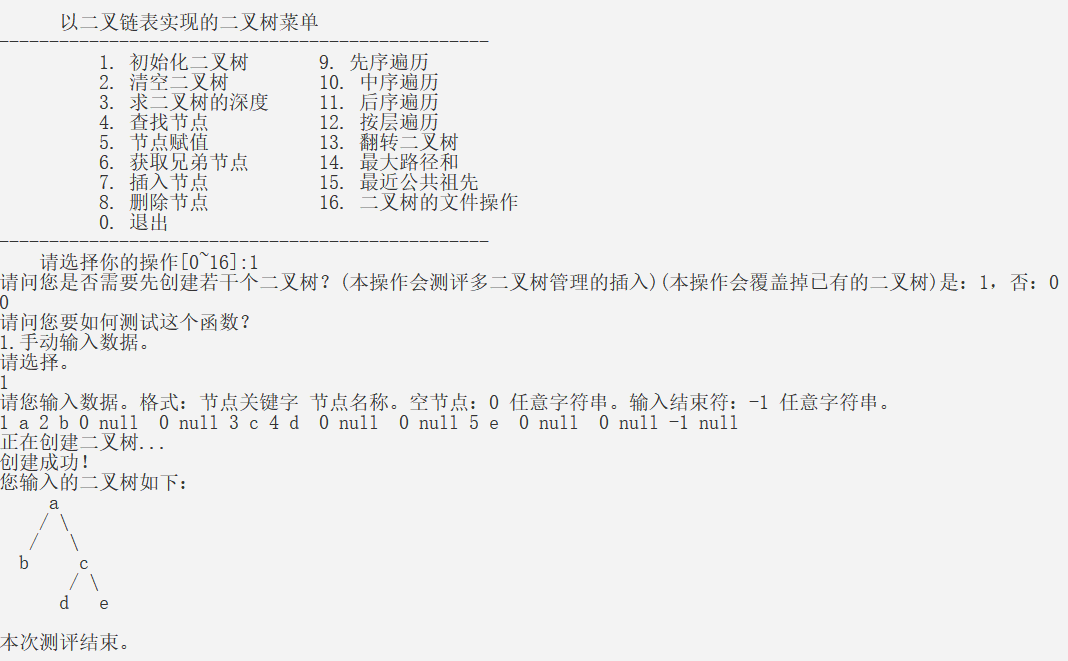
\includegraphics[scale=0.50]{images/二叉树-创建.png}
				\caption{二叉树-创建测试}
				\label{fig2-1}
			\end{center}
		\end{figure}
	\item 清空二叉树\\
	输入二叉树A,输出结果如下图:
		\begin{figure}[htb]
			\begin{center}
				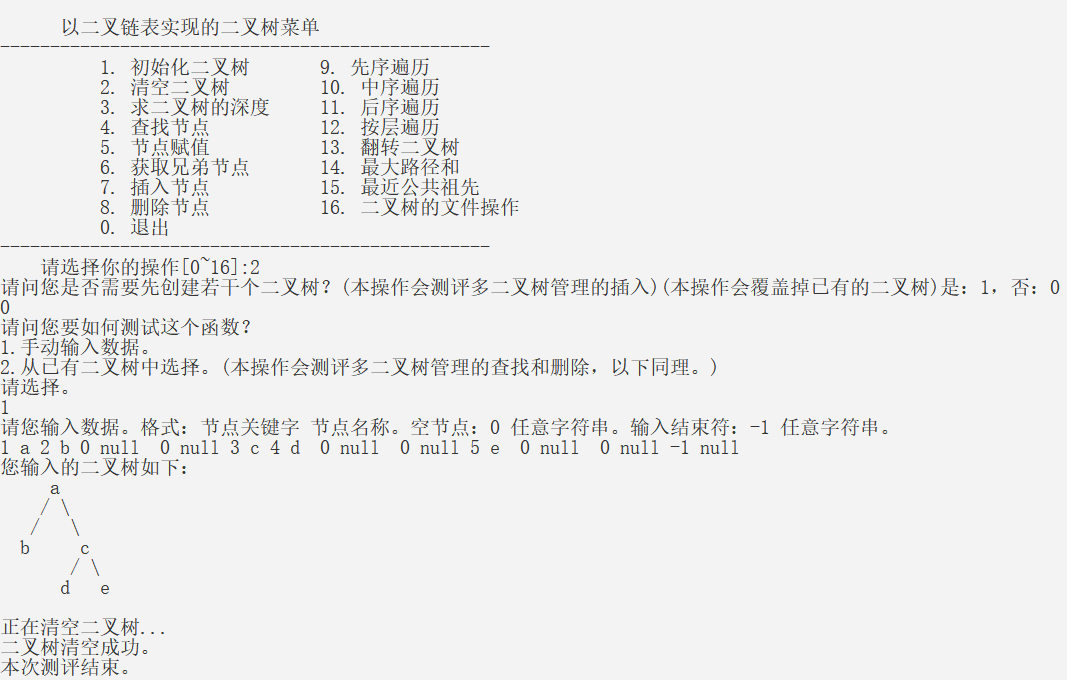
\includegraphics[scale=0.50]{images/二叉树-清空.png}
				\caption{二叉树-清空测试}
				\label{fig2-2}
			\end{center}
		\end{figure}
		\newpage
	\item 求二叉树的深度\\
	从二叉树的管理表中获得二叉树A,输出结果如下图:
		\begin{figure}[htb]
			\begin{center}
				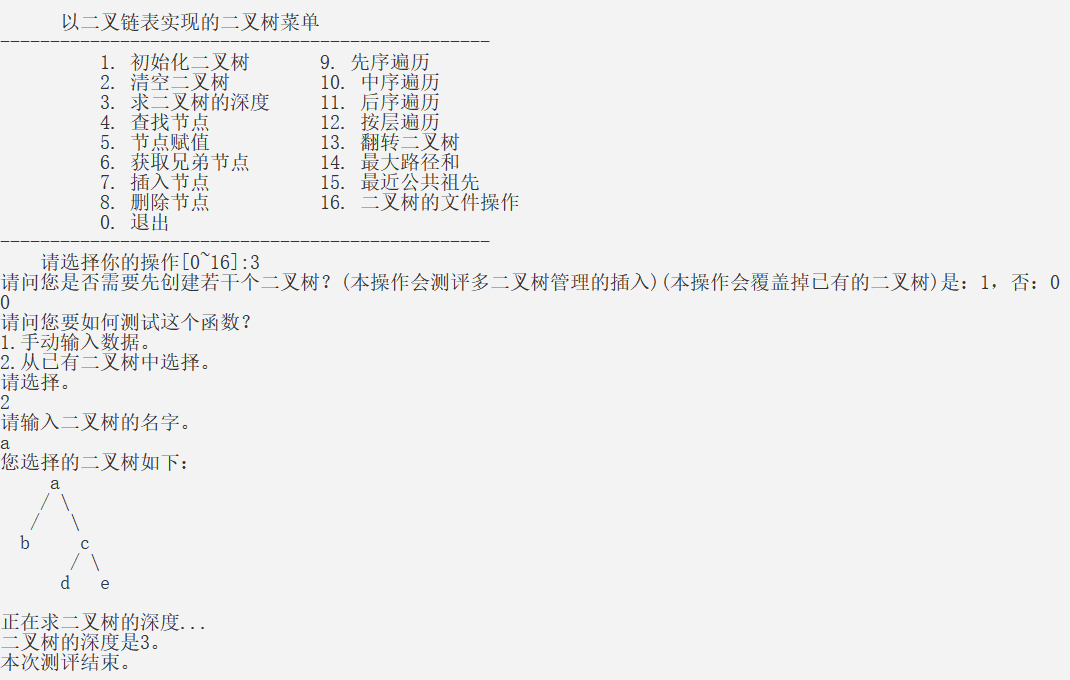
\includegraphics[scale=0.50]{images/二叉树-求深度.png}
				\caption{二叉树-求深度测试}
				\label{fig2-3}
			\end{center}
		\end{figure}
	\item 查找结点\\
	从二叉树的管理表中获得二叉树A,输出结果如下图:
		\begin{figure}[htb]
			\begin{center}
				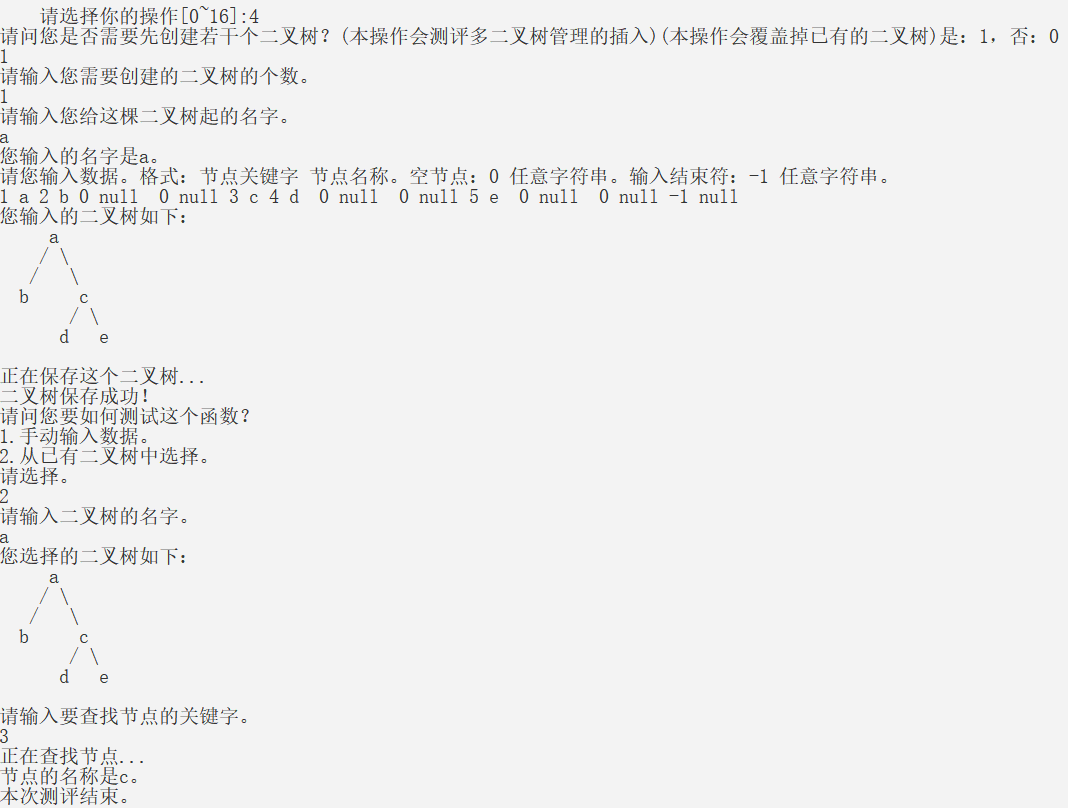
\includegraphics[scale=0.50]{images/二叉树-查找节点.png}
				\caption{二叉树-查找结点测试}
				\label{fig2-4}
			\end{center}
		\end{figure}
		\newpage
	\item 结点赋值\\
	输入二叉树A,输出结果如下图:
		\begin{figure}[htb]
			\begin{center}
				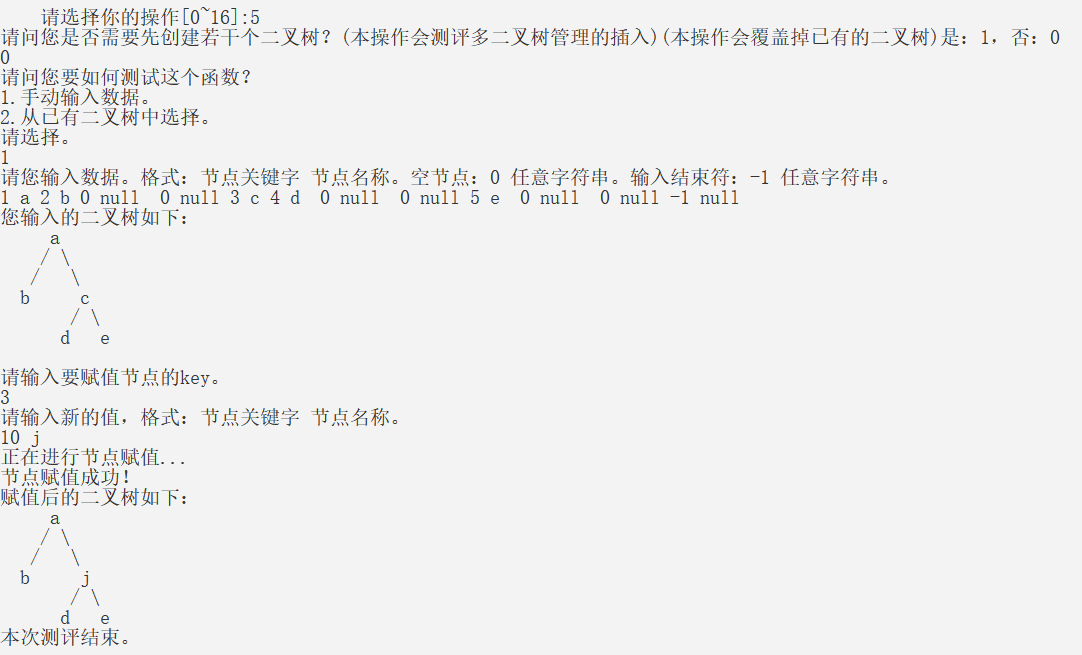
\includegraphics[scale=0.50]{images/二叉树-节点赋值.png}
				\caption{二叉树-结点赋值测试1}
				\label{fig2-5.1}
			\end{center}
		\end{figure}
		\begin{figure}[htb]
			\begin{center}
				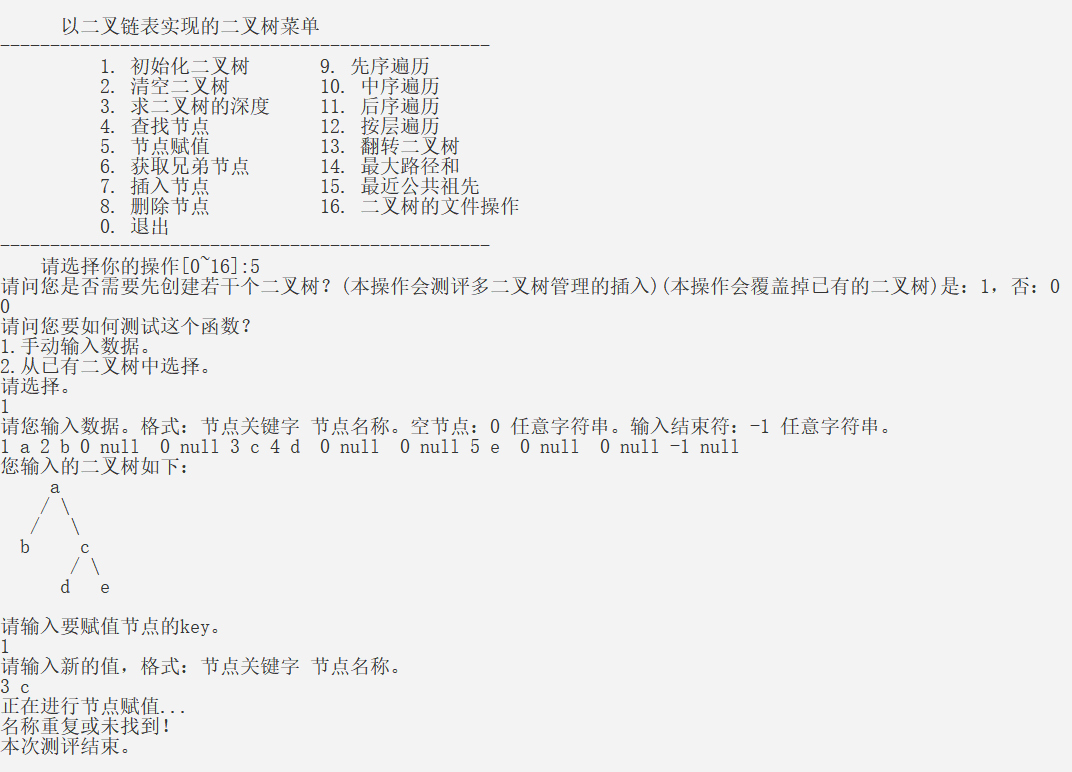
\includegraphics[scale=0.50]{images/二叉树-节点赋值异常.png}
				\caption{二叉树-结点赋值测试2}
				\label{fig2-5.2}
			\end{center}
		\end{figure}
		\newpage
	\item 获取兄弟结点\\
	从二叉树的管理表中获得二叉树A,输出结果如下图:
		\begin{figure}[htb]
			\begin{center}
				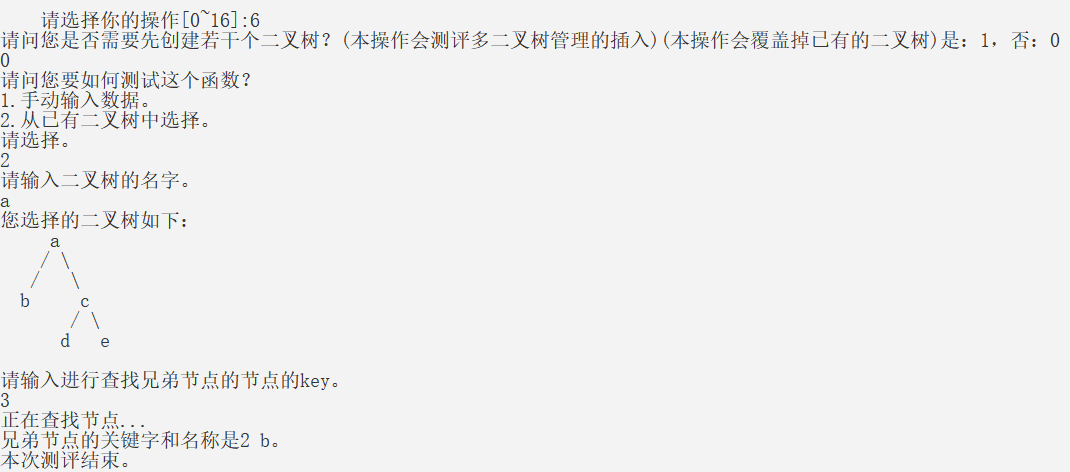
\includegraphics[scale=0.50]{images/二叉树-获取兄弟节点.png}
				\caption{二叉树-获取兄弟结点测试1}
				\label{fig2-6.1}
			\end{center}
		\end{figure}
		\begin{figure}[htb]
			\begin{center}
				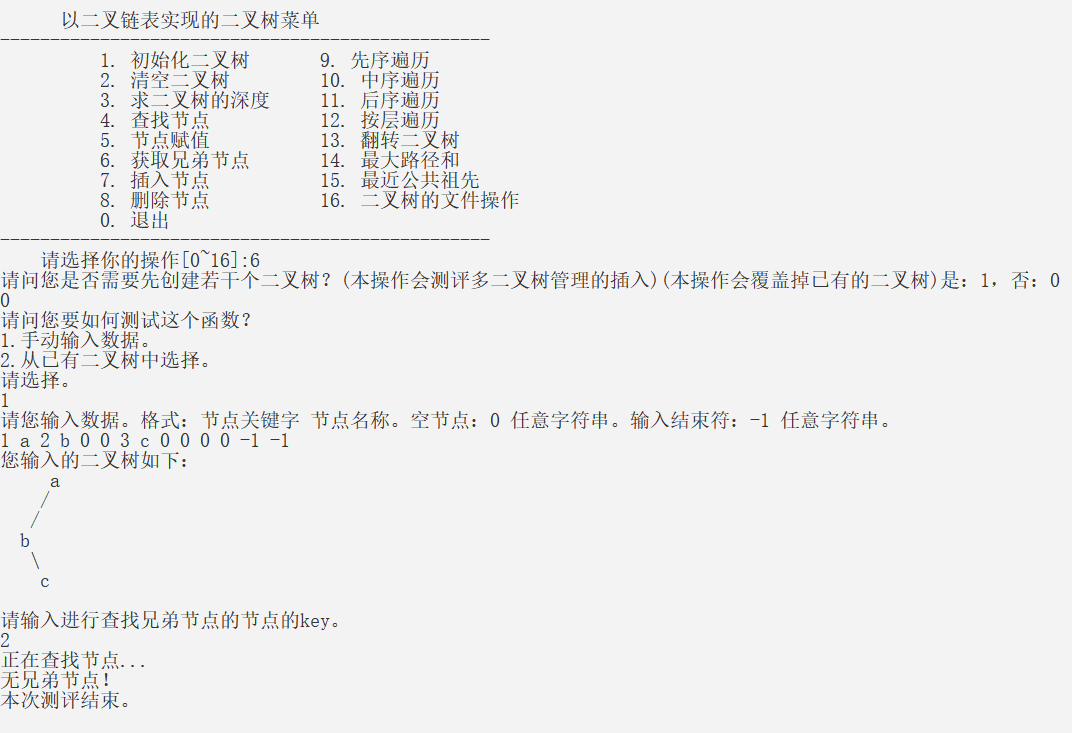
\includegraphics[scale=0.50]{images/二叉树-获取兄弟节点异常.png}
				\caption{二叉树-获取兄弟结点测试2}
				\label{fig2-6.2}
			\end{center}
		\end{figure}
		\newpage
	\item 插入结点\\
	输入二叉树A,输出结果如下图:
		\begin{figure}[htb]
			\begin{center}
				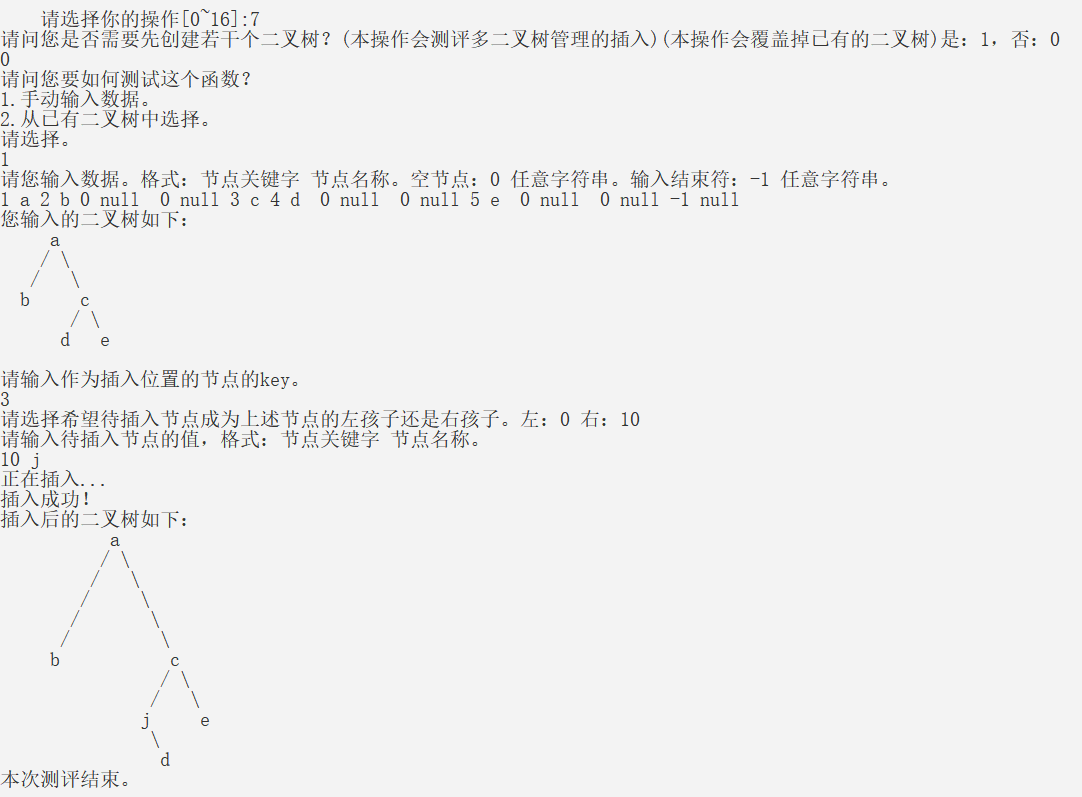
\includegraphics[scale=0.50]{images/二叉树-插入节点.png}
				\caption{二叉树-插入结点测试}
				\label{fig2-7}
			\end{center}
		\end{figure}
	\item 删除结点\\
	输入二叉树A,输出结果如下图:
		\begin{figure}[htb]
			\begin{center}
				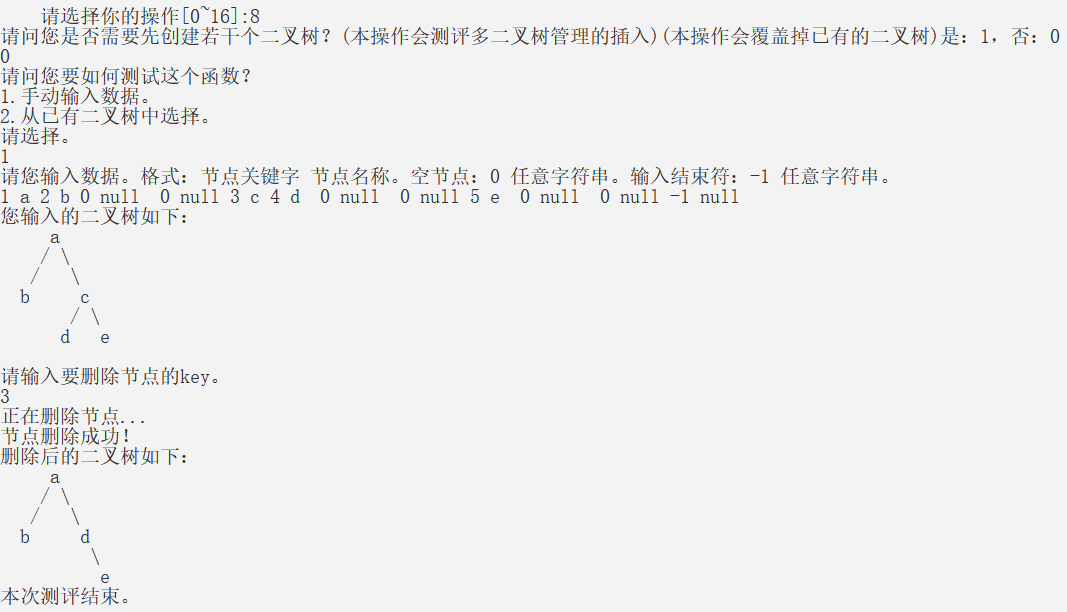
\includegraphics[scale=0.50]{images/二叉树-删除节点.png}
				\caption{二叉树-删除结点测试}
				\label{fig2-8}
			\end{center}
		\end{figure}
		\newpage
	\item 先序遍历\\
	从二叉树的管理表中获得二叉树A,输出结果如下图:
		\begin{figure}[htb]
			\begin{center}
				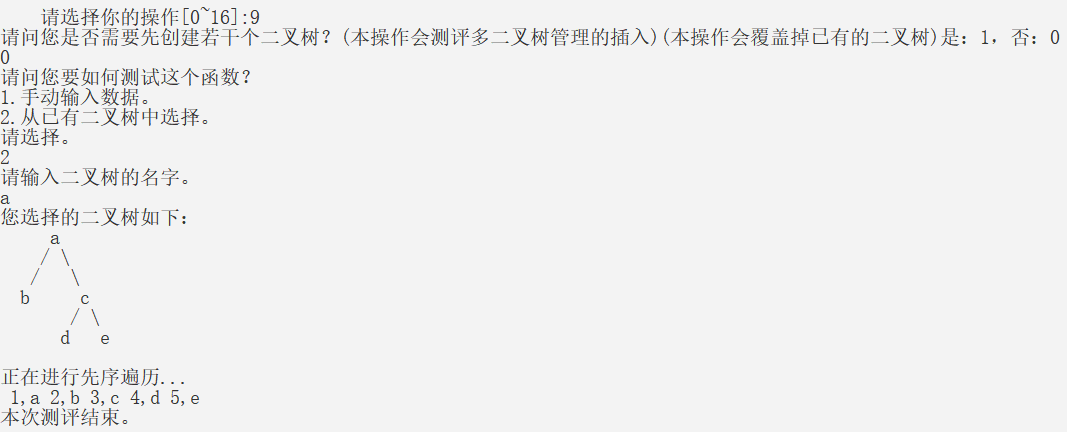
\includegraphics[scale=0.50]{images/二叉树-先序遍历.png}
				\caption{二叉树-先序遍历测试}
				\label{fig2-9}
			\end{center}
		\end{figure}
	\item 中序遍历\\
	从二叉树的管理表中获得二叉树A,输出结果如下图:
		\begin{figure}[htb]
			\begin{center}
				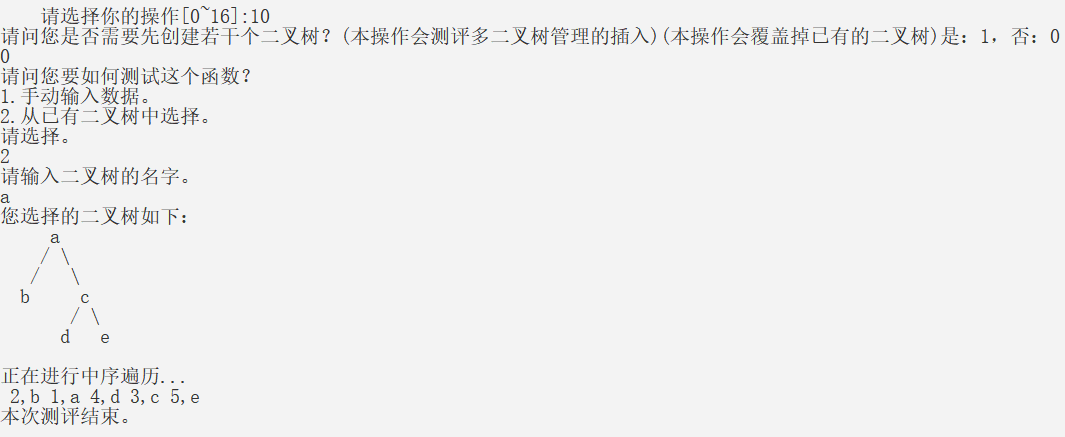
\includegraphics[scale=0.50]{images/二叉树-中序遍历.png}
				\caption{二叉树-中序遍历测试}
				\label{fig2-10}
			\end{center}
		\end{figure}
		\newpage
	\item 后序遍历\\
	从二叉树的管理表中获得二叉树A,输出结果如下图:
		\begin{figure}[htb]
			\begin{center}
				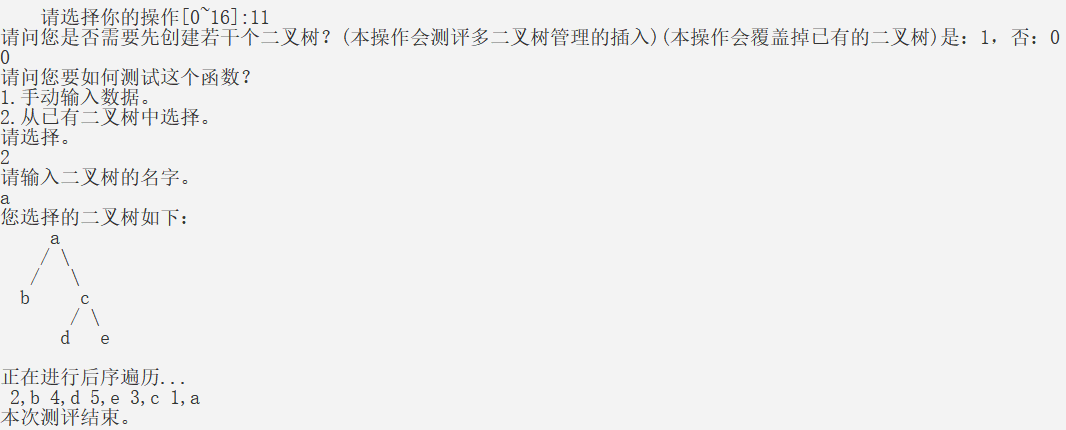
\includegraphics[scale=0.50]{images/二叉树-后序遍历.png}
				\caption{二叉树-后序遍历测试}
				\label{fig2-11}
			\end{center}
		\end{figure}
	\item 按层遍历\\
	从二叉树的管理表中获得二叉树A,输出结果如下图:
		\begin{figure}[htb]
			\begin{center}
				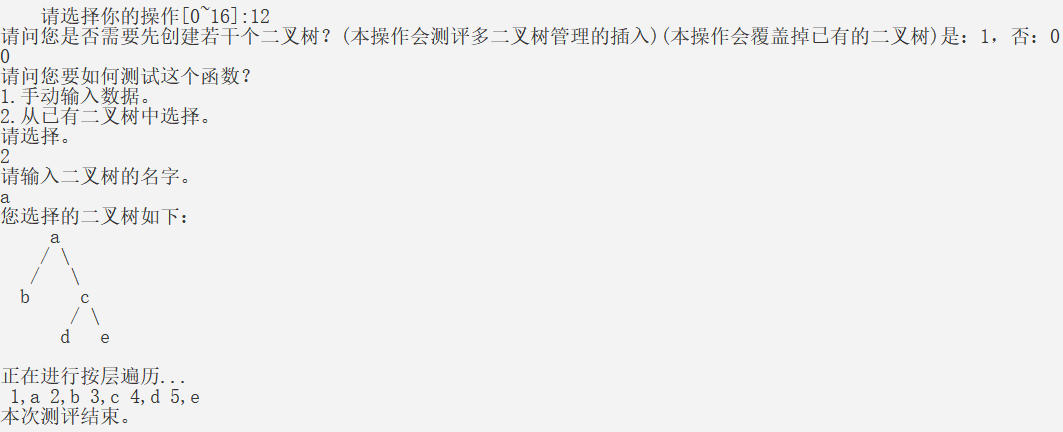
\includegraphics[scale=0.50]{images/二叉树-按层遍历.png}
				\caption{二叉树-按层遍历测试}
				\label{fig2-12}
			\end{center}
		\end{figure}
		\newpage
	\item 翻转二叉树\\
	输入二叉树A,输出结果如下图:
		\begin{figure}[htb]
			\begin{center}
				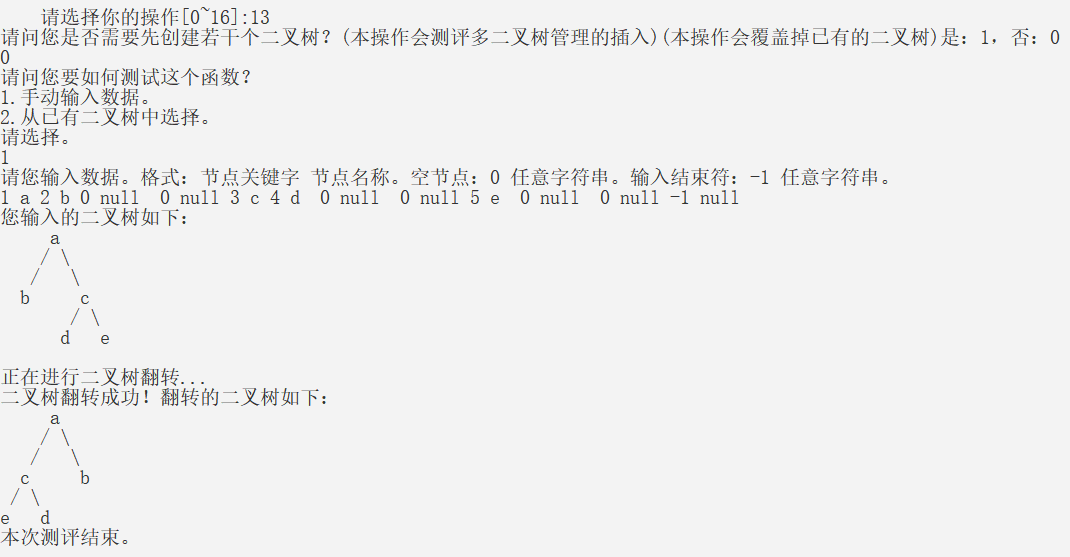
\includegraphics[scale=0.50]{images/二叉树-翻转.png}
				\caption{二叉树-翻转测试}
				\label{fig2-13}
			\end{center}
		\end{figure}
	\item 最大路径和\\
	从二叉树的管理表中获得二叉树A,输出结果如下图:
		\begin{figure}[htb]
			\begin{center}
				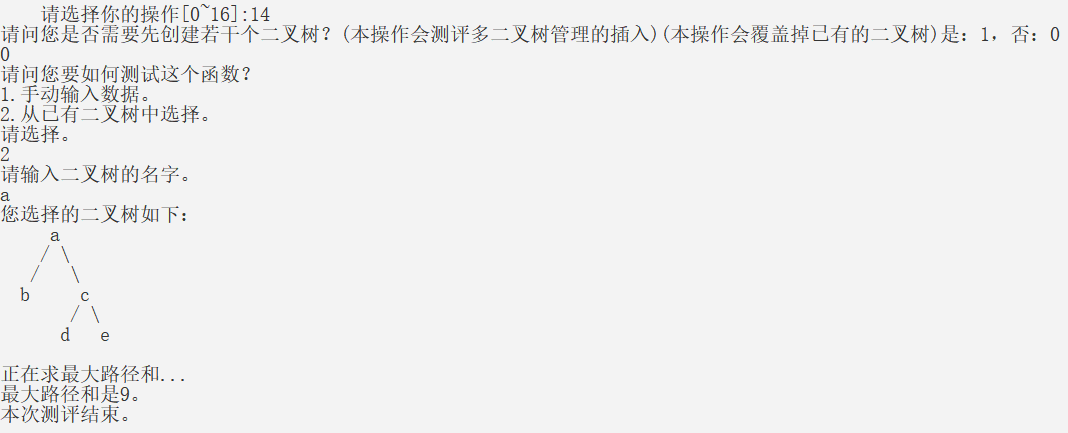
\includegraphics[scale=0.50]{images/二叉树-最大路径和.png}
				\caption{二叉树-最大路径和测试}
				\label{fig2-14}
			\end{center}
		\end{figure}
	\newpage
	\item 最近公共祖先\\
	从二叉树的管理表中获得二叉树A,输出结果如下图:
		\begin{figure}[htb]
			\begin{center}
				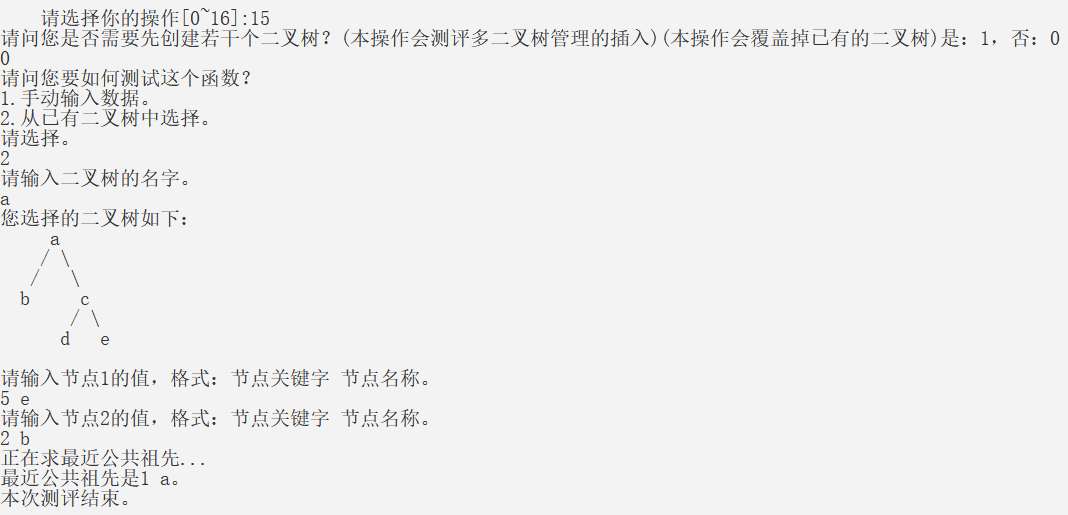
\includegraphics[scale=0.50]{images/二叉树-最近公共祖先.png}
				\caption{二叉树-最近公共祖先测试1}
				\label{fig2-15.1}
			\end{center}
		\end{figure}
		\begin{figure}[htb]
			\begin{center}
				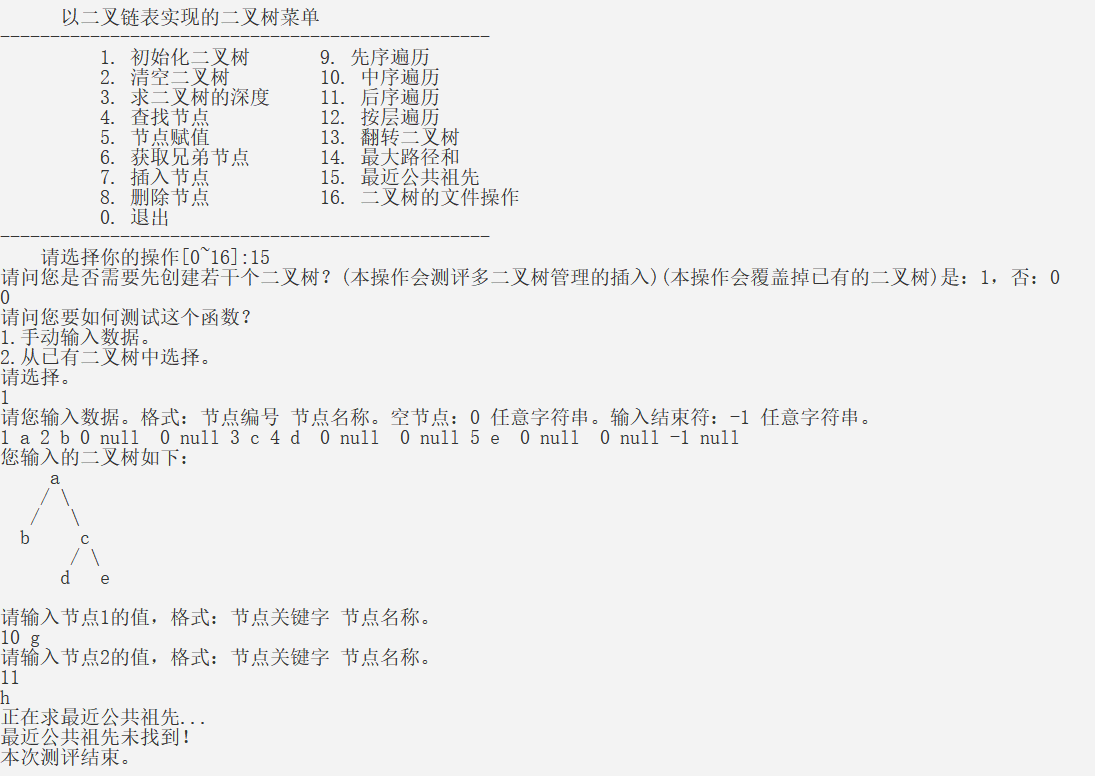
\includegraphics[scale=0.50]{images/二叉树-最近公共祖先异常.png}
				\caption{二叉树-最近公共祖先测试2}
				\label{fig2-15.2}
			\end{center}
		\end{figure}
		\newpage
	\item 二叉树的文件操作\\
	从二叉树的管理表中获得二叉树A,输出结果如下图:
		\begin{figure}[htb]
			\begin{center}
				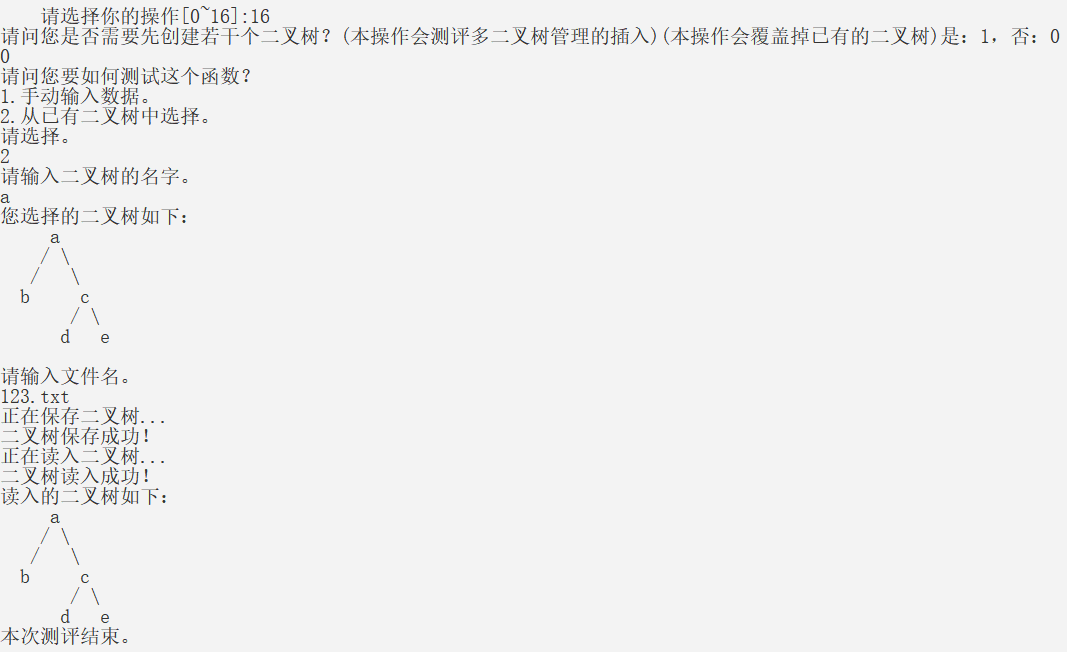
\includegraphics[scale=0.50]{images/二叉树-文件操作.png}
				\caption{二叉树-文件操作测试}
				\label{fig2-16.1}
			\end{center}
		\end{figure}
		\begin{figure}[htb]
			\begin{center}
				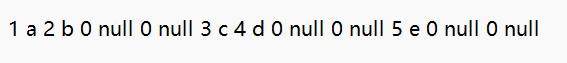
\includegraphics[scale=1.50]{images/二叉树-文件.png}
				\caption{二叉树-文件操作测试}
				\label{fig2-16.2}
			\end{center}
		\end{figure}
		\newpage
		\item 多二叉树管理\\
		输入二叉树A,输出结果如下图:
		\begin{figure}[htb]
			\begin{center}
				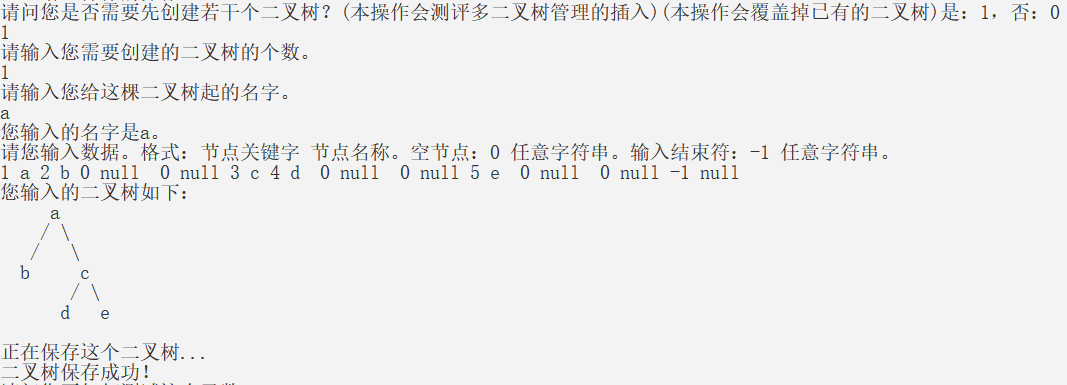
\includegraphics[scale=0.50]{images/二叉树-多二叉树管理.png}
				\caption{二叉树-多二叉树管理测试}
				\label{fig2-17}
			\end{center}
		\end{figure}
\end{enumerate}
\subsection{实验小结}
通过本次实验,我加深了对二叉链表存储的二叉树的理解,并掌握了如何运用二叉树解决实际问题。
通过本次实验,我学到了:
\begin{enumerate}
	\item 二叉链表的定义
    \item 二叉链表的基本操作算法
	\item 二叉链表存储的二叉树的定义
    \item 二叉链表存储的二叉树的基本操作算法
    \item 二叉树的管理表的定义
    \item 二叉树的管理表的基本操作算法
    \item 二叉树的实际应用
\end{enumerate}
通过本次实验,我认为我还有如下不足之处:
\begin{enumerate}
	\item 对其他结构存储的二叉树操作不够熟练
    \item 对二叉树的复杂操作不够熟练
\end{enumerate}
\newpage


\section{课程的收获和建议}


\subsection{基于顺序存储结构的线性表实现}

我的收获:
\begin{enumerate}
	\item 加深了对顺序表存储的线性表的理解
    \item 掌握了如何运用线性表解决实际问题
    \item 学到了顺序表的定义
    \item 学到了顺序表的基本操作算法
\end{enumerate}
我的建议:
\begin{enumerate}
	\item 增加一些有实际应用背景的实验内容
    \item 减少一些过于基础的实验内容
\end{enumerate}

\subsection{基于链式存储结构的线性表实现}

我的收获:
\begin{enumerate}
	\item 加深了对链式存储的线性表的理解
    \item 掌握了如何运用线性表解决实际问题
    \item 学到了单链表的定义
    \item 学到了单链表的基本操作算法
    \item 学到了单链表的管理表的定义
    \item 学到了单链表的管理表的基本操作算法
\end{enumerate}
我的建议:
\begin{enumerate}
	\item 增加一些有实际应用背景的实验内容
    \item 增加一些有关next指针操作的实验内容
    \item 减少一些过于基础的实验内容
\end{enumerate}

\subsection{基于二叉链表的二叉树实现}

我的收获:
\begin{enumerate}
	\item 加深了对二叉链表存储的二叉树的理解
    \item 掌握了如何运用二叉树解决实际问题
    \item 学到了二叉链表的定义
    \item 学到了二叉链表的基本操作算法
    \item 学到了二叉树的管理表的定义
    \item 学到了二叉树的管理表的基本操作算法
\end{enumerate}
我的建议:
\begin{enumerate}
	\item 增加一些有实际应用背景的实验内容
    \item 增加一些以其它存储方式实现的二叉树的实验
    \item 增加有关堆的操作
\end{enumerate}

\subsection{基于邻接表的图实现}

我的收获:
\begin{enumerate}
	\item 加深了对图的理解
    \item 掌握了如何图解决实际问题
    \item 学到了邻接表的定义
    \item 学到了邻接表的基本操作算法
    \item 学到了图的管理表的定义
    \item 学到了图的管理表的基本操作算法
\end{enumerate}
我的建议:
\begin{enumerate}
	\item 增加一些有实际应用背景的实验内容
    \item 增加一些以其它存储方式实现的图的实验
\end{enumerate}

\newpage
\section{参考文献}
\begin{enumerate}
	\item 严蔚敏等.数据结构(C语言版).清华大学出版社
    \item Larry Nyhoff. ADTs, Data Structures, and Problem Solving with C++. Second Edition,Calvin College,2005
	\item 殷立峰. Qt C++跨平台图形界面程序设计基础. 清华大学出版社,2014:192~197
    \item 严蔚敏等.数据结构题集(C语言版).清华大学出版社
\end{enumerate}
\newpage

\section{附录A 基于顺序存储结构线性表实现的源程序}
\begin{lstlisting}[title =def,frame=none]
#include<stdio.h>
#include<stdlib.h>
#include<string.h>
#include<time.h>
#define TRUE 1
#define FALSE 0
#define OK 1
#define ERROR 0
#define INFEASIBLE -1
#define OVERFLOW -2
typedef int status;
typedef int ElemType; //数据元素类型定义
#define LIST_INIT_SIZE 100
#define LISTINCREMENT  10
typedef int ElemType;
typedef struct  //顺序表(顺序结构)的定义
{
ElemType * elem;//元素。 
int length;//表长。 
int listsize;//最大长度。 
}SqList;
typedef struct{  //线性表的管理表定义
    struct//名字和线性表。 
	{
		char name[30];
    	SqList L;	
    }elem[10];
    int length;//管理表长。 
    int listsize;//管理表最大长度。 
}LISTS;
\end{lstlisting}
\begin{lstlisting}[title =演示系统,frame=none]
	#include"../def.h"
	#include"../顺序表-遍历.h"
	#include"../顺序表-插入.h"
	#include"../顺序表-查找元素.h"
	#include"../顺序表-初始化.h"
	#include"../顺序表-查找后继元素.h"
	#include"../顺序表-查找前驱元素.h"
	#include"../顺序表-获取元素.h"
	#include"../顺序表-判空.h"
	#include"../顺序表-清空.h"
	#include"../顺序表-求表长.h"
	#include"../顺序表-删除.h"
	#include"../顺序表-文件操作.h"
	#include"../顺序表-销毁.h"
	#include"../多顺序表管理-移除一个顺序表.h"
	#include"../多顺序表管理-增加一个新顺序表.h"
	#include"../多线性表管理-查找顺序表.h"
	#include"../附加功能/顺序表-和为k的子数组个数.h"
	#include"../附加功能/顺序表-最大连续子数组和.h"
	#include"../附加功能/顺序表-排序.h"
	#include"顺序表数据构造器.h"
	int main()
	{
	int i=0,j=0,op1=1,op2=0,op3=0,sign=0,n=0,ret=0;
	int len[3]={0,10000,1000000};
	const char*namelist[3]={"test0.txt","test1.txt","test2.txt"};
	const char*rnamelist[3]={"result0.txt","result1.txt","result2.txt"};
	SqList L;
	LISTS list_table;
	char name[20];
	while(op1)
	{
		system("cls");	printf("\n\n");
		printf("      以顺序表实现的线性表菜单 \n");
		printf("-------------------------------------------------\n");
		printf("    	  1. 初始化线性表       9. 查找元素\n");
		printf("    	  2. 销毁线性表         10. 获取前驱元素\n");
		printf("    	  3. 清空线性表         11. 获取后继元素 \n");
		printf("    	  4. 判定线性表是否为空 12. 插入元素\n");
		printf("    	  5. 求线性表的长度     13. 删除元素\n");
		printf("    	  6. 获取元素           14. 遍历线性表\n");
		printf("    	  7. 和为k的子数组个数  15. 最大连续子数组和\n");
		printf("    	  8. 排序线性表         16. 线性表的文件操作\n");
		printf("    	  0. 退出\n");
		printf("-------------------------------------------------\n");
		printf("    请选择你的操作[0~16]:");
		scanf("%d",&op1);
		L.elem=NULL;
		L.length=0;
		if(op1<0||op1>16)
		{
			printf("Invalid Input!\n");
			system("pause");
			exit(-1);
		}
		printf("请问您是否需要先创建若干个线性表?(本操作会测评多线性表管理的插入)(本操作会覆盖掉已有的线性表)是:1,否:0\n");
		scanf("%d",&op2);
		if(op2!=1&&op2!=0)
		{
			printf("Invalid Input!\n");
			system("pause");
			exit(-1);
		}
		if(op2==1)//创建线性表的管理表。 
		{
			list_table.length=0;
			list_table.listsize=LISTINCREMENT;//初始化list_table。 
			printf("请输入您需要创建的线性表的个数。\n"); 
			scanf("%d",&n);
			if(n>LISTINCREMENT)//n太大。 
			{
				printf("OVERFLOW!\n");
				system("pause");
				exit(-1);
			}
			for(j=0;j<n;j++)
			{
				printf("请输入您给这个线性表起的名字。\n");
				scanf("%s",&name);
				printf("您输入的名字是%s。\n",name);
				printf("请您输入数据,以0结尾。\n");
				L.elem=(ElemType *) malloc(sizeof(ElemType)*LIST_INIT_SIZE);
				 L.length=0;
				 L.listsize=LIST_INIT_SIZE;
				 scanf("%d",&i);
				 while (i)
				 {
					 if(L.length==L.listsize)
					 {
						 printf("线性表已满,不再接收数据!\n");
						break; 
					}
					 L.elem[L.length++]=i;
					 scanf("%d",&i);
				 } 
				printf("您输入的线性表如下:\n");
				ListTraverse(L);
				printf("\n");
				printf("正在保存这个线性表...\n");
				sign=AddList(list_table,L,name); 
				if(sign==OK){printf("线性表保存成功!\n");}
				else if(sign==ERROR){printf("名字重复!\n");}
				else{printf("线性表保存失败!\n");}
				DestroyList(L);
			}
		}
		switch(op1)
		{
		   case 1://创建线性表。 
			printf("请问您要如何测试这个函数?\n");
			printf("1.手动输入数据。\n"); 
			printf("请选择。\n");
			scanf("%d",&op3);
			if(op3!=1)
			{
				printf("Invalid Input!");
				break;
			}
			if(op3==1)//手动输入数据。 
			{
				printf("请您输入数据,以0结尾。\n");
				/*L=(LinkList)malloc(sizeof(LNode));
				L->next=NULL;*/
				sign=InitList(L);
				scanf("%d",&i);
				 while (i)
				 {
					 if(L.length==L.listsize)
					 {
						 printf("线性表已满,不再接收数据!\n");
						break; 
					}
					 L.elem[L.length++]=i;
					 scanf("%d",&i);
				 } 
				if(sign==OK)
				{
					printf("线性表创建成功!\n");
					printf("您输入的线性表如下:\n");
					ListTraverse(L);
					printf("\n");
				}
				else
				{
					printf("线性表创建失败!\n");
					DestroyList(L);
				}
				printf("本次测评结束。\n"); 
			}
			DestroyList(L);
			getchar();getchar();
			break;
		   case 2://销毁线性表。 
			printf("请问您要如何测试这个函数?\n");
			printf("1.自动测试。\n2.手动输入数据。\n3.从已有线性表中选择。(本操作会测评多线性表管理的查找和删除,以下同理。)\n"); 
			printf("请选择。\n");
			scanf("%d",&op3);
			if(op3<=0||op3>3)
			{
				printf("Invalid Input!");
				break;
			}
			if(op3==1)//自动测试。 
			{
				for(i=0;i<3;i++)
				{
					createdataforsqlist(L,len[i],namelist[i]);
					printf("本次测试数据集的个数是%d。\n",len[i]);
					sign=DestroyList(L);
					if(sign==OK)
					{
						printf("线性表销毁成功!\n");
						printf("\n");
					}
					else{printf("线性表销毁失败!\n");}
					DestroyList(L);
				}
			}
			else if(op3==2)//手动输入数据。 
			{
				printf("请您输入数据,以0结尾。\n");
				L.elem=(ElemType *) malloc(sizeof(ElemType)*LIST_INIT_SIZE);
				 L.length=0;
				 L.listsize=LIST_INIT_SIZE;
				 scanf("%d",&i);
				 while(i)
				 {
					 if(L.length==L.listsize)
					 {
						 printf("线性表已满,不再接收数据!\n");
						break; 
					}
					 L.elem[L.length++]=i;
					 scanf("%d",&i);
				 } 
				printf("您输入的线性表如下:\n");
				ListTraverse(L);
				printf("\n");
				printf("正在销毁线性表...\n"); 
				sign=DestroyList(L);
				if(sign==OK){printf("线性表销毁成功!\n");}
				else{printf("线性表销毁失败!\n");}
				printf("本次测评结束。\n");
			}
			else//从已有链表中选择。 
			{
				if(list_table.elem==NULL)
				{
					printf("没有已有线性表!\n");
					break;
				}
				printf("请输入线性表的名字。\n");
				scanf("%s",&name);
				i=LocateList(list_table,name);
				if(i==0)
				{
					printf("未找到线性表!\n");
					break;
				}
				printf("您选择的线性表如下:\n");
				ListTraverse(list_table.elem[i-1].L);
				printf("\n");
				printf("正在销毁线性表...\n");
				sign=DestroyList(list_table.elem[i-1].L);
				if(sign==OK){printf("线性表销毁成功!\n");}
				else{printf("线性表创建失败!\n");}
				printf("正在从管理表中删除...\n");
				sign=RemoveList(list_table,name);
				if(sign==OK){printf("删除成功!\n");}
				else{printf("删除失败!\n");}
				printf("本次测评结束。\n");
			}
			getchar();getchar();
			break;
		   case 3://清空线性表。 
			printf("请问您要如何测试这个函数?\n");
			printf("1.自动测试。\n2.手动输入数据。\n3.从已有线性表中选择。\n"); 
			printf("请选择。\n");
			scanf("%d",&op3);
			if(op3<=0||op3>3)
			{
				printf("Invalid Input!");
				break;
			}
			if(op3==1)
			{
				for(i=0;i<3;i++)
				{
					createdataforsqlist(L,len[i],namelist[i]);
					printf("本次测试数据集的个数是%d。\n",len[i]);
					sign=ClearList(L);
					if(sign==OK)
					{
						printf("线性表清空成功!\n");
						printf("\n");
					}
					else{printf("线性表清空失败!\n");}
					DestroyList(L);
				}
			}
			else if(op3==2)//手动输入数据。 
			{
				printf("请您输入数据,以0结尾。\n");
				L.elem=(ElemType *) malloc(sizeof(ElemType)*LIST_INIT_SIZE);
				 L.length=0;
				 L.listsize=LIST_INIT_SIZE;
				 scanf("%d",&i);
				 while(i)
				 {
					 if(L.length==L.listsize)
					 {
						 printf("线性表已满,不再接收数据!\n");
						break; 
					}
					 L.elem[L.length++]=i;
					 scanf("%d",&i);
				 } 
				printf("您输入的线性表如下:\n");
				ListTraverse(L);
				printf("\n");
				printf("正在清空线性表...\n"); 
				sign=ClearList(L);
				if(sign==OK){printf("线性表清空成功!\n");}
				else{printf("线性表清空失败!\n");}
				printf("本次测评结束。\n");
				DestroyList(L);
			}
			else//从已有链表中选择。 
			{
				if(list_table.elem==NULL)
				{
					printf("没有已有线性表!\n");
					break;
				}
				printf("请输入线性表的名字。\n");
				scanf("%s",&name);
				i=LocateList(list_table,name);
				if(i==0)
				{
					printf("未找到线性表!\n");
					break;
				}
				printf("您选择的线性表如下:\n");
				ListTraverse(list_table.elem[i-1].L);
				printf("\n");
				printf("正在清空线性表...\n");
				sign=ClearList(list_table.elem[i-1].L);
				if(sign==OK){printf("线性表清空成功!\n");}
				else{printf("线性表清空失败!\n");}
				printf("本次测评结束。\n"); 
			}
			getchar();getchar();
			break;
		   case 4://判空线性表。 
			printf("请问您要如何测试这个函数?\n");
			printf("1.自动测试。\n2.手动输入数据。\n3.从已有线性表中选择。\n"); 
			printf("请选择。\n");
			scanf("%d",&op3);
			if(op3<=0||op3>3)
			{
				printf("Invalid Input!");
				break;
			}
			if(op3==1)
			{
				for(i=0;i<3;i++)
				{
					createdataforsqlist(L,len[i],namelist[i]);
					printf("本次测试数据集的个数是%d。\n",len[i]);
					sign=ListEmpty(L);
					if(sign==TRUE){printf("线性表为空。\n");}
					else if(sign==FALSE){printf("线性表不为空。\n");}
					else{printf("线性表判空失败!\n");}
					printf("本次测评结束。\n");
					DestroyList(L);
				}
			}
			else if(op3==2)//手动输入数据。 
			{
				printf("请您输入数据,以0结尾。\n");
				L.elem=(ElemType *) malloc(sizeof(ElemType)*LIST_INIT_SIZE);
				 L.length=0;
				 L.listsize=LIST_INIT_SIZE;
				 scanf("%d",&i);
				 while(i)
				 {
					 if(L.length==L.listsize)
					 {
						 printf("线性表已满,不再接收数据!\n");
						break; 
					}
					 L.elem[L.length++]=i;
					 scanf("%d",&i);
				 } 
				printf("您输入的线性表如下:\n");
				ListTraverse(L);
				printf("\n");
				printf("正在进行线性表的判空...\n"); 
				sign=ListEmpty(L);
				if(sign==TRUE){printf("线性表为空。\n");}
				else if(sign==FALSE){printf("线性表不为空。\n");}
				else{printf("线性表判空失败!\n");}
				printf("本次测评结束。\n");
				DestroyList(L);
			}
			else//从已有链表中选择。 
			{
				if(list_table.length==0)
				{
					printf("没有已有线性表!\n");
					break;
				}
				printf("请输入线性表的名字。\n");
				scanf("%s",&name);
				i=LocateList(list_table,name);
				if(i==0)
				{
					printf("未找到线性表!\n");
					break;
				}
				printf("您选择的线性表如下:\n");
				ListTraverse(list_table.elem[i-1].L);
				printf("\n");
				printf("正在进行线性表的判空...\n"); 
				sign=ListEmpty(list_table.elem[i-1].L);
				if(sign==TRUE){printf("线性表为空。\n");}
				else if(sign==FALSE){printf("线性表不为空。\n");}
				else{printf("线性表判空失败!\n");}
				printf("本次测评结束。\n");
			}
			getchar();getchar();
			break;
		   case 5://求表长 
			printf("请问您要如何测试这个函数?\n");
			printf("1.自动测试。\n2.手动输入数据。\n3.从已有线性表中选择。\n"); 
			printf("请选择。\n");
			scanf("%d",&op3);
			if(op3<=0||op3>3)
			{
				printf("Invalid Input!");
				break;
			}
			if(op3==1)
			{
				for(i=0;i<3;i++)
				{
					createdataforsqlist(L,len[i],namelist[i]);
					printf("本次测试数据集的个数是%d。\n",len[i]);
					ret=ListLength(L);
					if(ret==INFEASIBLE){printf("INFEASIBLE!\n");}
					else{printf("线性表的长度是%d。\n",ret);}
					printf("本次测评结束。\n"); 
					DestroyList(L);
				}
			}
			else if(op3==2)//手动输入数据。 
			{
				printf("请您输入数据,以0结尾。\n");
				L.elem=(ElemType *) malloc(sizeof(ElemType)*LIST_INIT_SIZE);
				 L.length=0;
				 L.listsize=LIST_INIT_SIZE;
				 scanf("%d",&i);
				 while(i)
				 {
					 if(L.length==L.listsize)
					 {
						 printf("线性表已满,不再接收数据!\n");
						break; 
					}
					 L.elem[L.length++]=i;
					 scanf("%d",&i);
				 } 
				printf("您输入的线性表如下:\n");
				ListTraverse(L);
				printf("\n");
				printf("正在求线性表的长度...\n"); 
				ret=ListLength(L);
				if(ret==INFEASIBLE){printf("INFEASIBLE!\n");}
				else{printf("线性表的长度是%d。\n",ret);}
				printf("本次测评结束。\n"); 
				DestroyList(L);
			}
			else//从已有链表中选择。 
			{
				if(list_table.length==0)
				{
					printf("没有已有线性表!\n");
					break;
				}
				printf("请输入线性表的名字。\n");
				scanf("%s",&name);
				i=LocateList(list_table,name);
				if(i==0)
				{
					printf("未找到线性表!\n");
					break;
				}
				printf("您选择的线性表如下:\n");
				ListTraverse(list_table.elem[i-1].L);
				printf("\n");
				printf("正在求线性表的长度...\n"); 
				ret=ListLength(list_table.elem[i-1].L);
				if(ret==INFEASIBLE){printf("INFEASIBLE!\n");}
				else{printf("线性表的长度是%d。\n",ret);}
				printf("本次测评结束。\n"); 
			}
			getchar();getchar();
			break;
		   case 6://获取元素。 
			printf("请问您要如何测试这个函数?\n"); 
			printf("1.自动测试。\n2.手动输入数据。\n3.从已有线性表中选择。\n"); 
			printf("请选择。\n");
			scanf("%d",&op3);
			if(op3<=0||op3>3)
			{
				printf("Invalid Input!");
				break;
			}
			if(op3==1)
			{
				for(i=0;i<3;i++)
				{
					createdataforsqlist(L,len[i],namelist[i]);
					printf("本次测试数据集的个数是%d。\n",len[i]);
					j=getrnum();
					printf("索引是%d。\n",j);
					sign=GetElem(L,j,ret);
					if(sign==INFEASIBLE){printf("空线性表!\n");}
					else if(sign==ERROR){printf("不合法的索引!\n");}
					else{printf("索引是%d的元素是%d。\n",j,ret);}
					printf("本次测评结束。\n");
					DestroyList(L);
				}
			}
			else if(op3==2)//手动输入数据。 
			{
				printf("请您输入数据,以0结尾。\n");
				L.elem=(ElemType *) malloc(sizeof(ElemType)*LIST_INIT_SIZE);
				 L.length=0;
				 L.listsize=LIST_INIT_SIZE;
				 scanf("%d",&i);
				 while(i)
				 {
					 if(L.length==L.listsize)
					 {
						 printf("线性表已满,不再接收数据!\n");
						break; 
					}
					 L.elem[L.length++]=i;
					 scanf("%d",&i);
				 } 
				printf("您输入的线性表如下:\n");
				ListTraverse(L);
				printf("\n");
				printf("请输入索引。\n");
				scanf("%d",&i); 
				printf("正在获取元素...\n"); 
				sign=GetElem(L,i,ret);
				if(sign==INFEASIBLE){printf("空线性表!\n");}
				else if(sign==ERROR){printf("不合法的索引!\n");}
				else{printf("索引是i的元素是%d。\n",ret);}
				printf("本次测评结束。\n"); 
				DestroyList(L);
			}
			else//从已有链表中选择。 
			{
				if(list_table.length==0)
				{
					printf("没有已有线性表!\n");
					break;
				}
				printf("请输入线性表的名字。\n");
				scanf("%s",&name);
				i=LocateList(list_table,name);
				if(i==0)
				{
					printf("未找到线性表!\n");
					break;
				}
				printf("您选择的线性表如下:\n");
				ListTraverse(list_table.elem[i-1].L);
				printf("\n");
				printf("请输入索引。\n");
				scanf("%d",&j); 
				printf("正在获取元素...\n"); 
				sign=GetElem(list_table.elem[i-1].L,j,ret);
				if(sign==INFEASIBLE){printf("空线性表!\n");}
				else if(sign==ERROR){printf("不合法的索引!\n");}
				else{printf("索引是%d的元素是%d。\n",j,ret);}
				printf("本次测评结束。\n"); 
			}
			getchar();getchar();
			break;
		   case 7://和为k子数组。 
			printf("请问您要如何测试这个函数?\n");
			printf("1.手动输入数据。\n2.从已有线性表中选择。\n"); 
			printf("请选择。\n");
			scanf("%d",&op3);
			if(op3<=0||op3>2)
			{
				printf("Invalid Input!");
				break;
			}
			if(op3==1)//手动输入数据。 
			{
				printf("请您输入数据,以0结尾。\n");
				L.elem=(ElemType *) malloc(sizeof(ElemType)*LIST_INIT_SIZE);
				 L.length=0;
				 L.listsize=LIST_INIT_SIZE;
				 scanf("%d",&i);
				 while(i)
				 {
					 if(L.length==L.listsize)
					 {
						 printf("线性表已满,不再接收数据!\n");
						break; 
					}
					 L.elem[L.length++]=i;
					 scanf("%d",&i);
				 } 
				printf("您输入的线性表如下:\n");
				ListTraverse(L);
				printf("\n");
				printf("请输入子数组和。\n");
				scanf("%d",&i);
				printf("正在求和为%d的子数组个数...\n",i); 
				ret=SubArrayNum(L,i);
				printf("和为%d的子数组个数是%d。\n",i,ret);
				printf("本次测评结束。\n");
				DestroyList(L);
			}
			else//从已有链表中选择。 
			{
				if(list_table.length==0)
				{
					printf("没有已有线性表!\n");
					break;
				}
				printf("请输入线性表的名字。\n");
				scanf("%s",&name);
				i=LocateList(list_table,name);
				if(i==0)
				{
					printf("未找到线性表!\n");
					break;
				}
				printf("您选择的线性表如下:\n");
				ListTraverse(list_table.elem[i-1].L);
				printf("\n");
				printf("请输入子数组和。\n");
				scanf("%d",&j);
				printf("正在求和为%d的子数组个数...\n",j); 
				ret=SubArrayNum(list_table.elem[i-1].L,j);
				printf("和为%d的子数组个数是%d。\n",j,ret);
				printf("本次测评结束。\n");
			}
			getchar();getchar();
			break;
		   case 8://排序线性表。 
			printf("请问您要如何测试这个函数?\n");
			printf("1.自动测试。\n2.手动输入数据。\n3.从已有线性表中选择。\n"); 
			printf("请选择。\n");
			scanf("%d",&op3);
			if(op3<=0||op3>3)
			{
				printf("Invalid Input!");
				break;
			}
			if(op3==1)
			{
				for(i=0;i<3;i++)
				{
					createdataforsqlist(L,len[i],namelist[i]);
					printf("本次测试数据集的个数是%d。\n",len[i]);
					sign=sortList(L);
					if(sign==OK)
					{
						printf("线性表排序成功!\n");
						savelistforsqlist(L,rnamelist[i]);
						printf("\n");
					}
					else{printf("线性表排序失败!\n");}
					printf("本次测评结束。\n");
					DestroyList(L);
				}
			}
			else if(op3==2)//手动输入数据。 
			{
				printf("请您输入数据,以0结尾。\n");
				L.elem=(ElemType *) malloc(sizeof(ElemType)*LIST_INIT_SIZE);
				 L.length=0;
				 L.listsize=LIST_INIT_SIZE;
				 scanf("%d",&i);
				 while(i)
				 {
					 if(L.length==L.listsize)
					 {
						 printf("线性表已满,不再接收数据!\n");
						break; 
					}
					 L.elem[L.length++]=i;
					 scanf("%d",&i);
				 } 
				printf("您输入的线性表如下:\n");
				ListTraverse(L);
				printf("\n");
				printf("正在进行线性表的排序...\n"); 
				if(L.elem==NULL){printf("空线性表。\n");}
				else
				{
					sortList(L);
					printf("排序后的线性表如下:\n");
					ListTraverse(L);
					printf("\n");
				}
				printf("本次测评结束。\n");
				DestroyList(L);
			}
			else//从已有链表中选择。 
			{
				if(list_table.length==0)
				{
					printf("没有已有线性表!\n");
					break;
				}
				printf("请输入线性表的名字。\n");
				scanf("%s",&name);
				i=LocateList(list_table,name);
				if(i==0)
				{
					printf("未找到线性表!\n");
					break;
				}
				printf("您选择的线性表如下:\n");
				ListTraverse(list_table.elem[i-1].L);
				printf("\n");
				printf("正在进行线性表的排序...\n"); 
				if(list_table.elem[i-1].L.elem==NULL){printf("空线性表。\n");}
				else
				{
					sortList(list_table.elem[i-1].L);
					printf("排序后的线性表如下:\n");
					ListTraverse(list_table.elem[i-1].L);
					printf("\n");
				}
				printf("本次测评结束。\n");
			}
			getchar();getchar();
			break;
		   case 9://查找元素。 
			printf("请问您要如何测试这个函数?\n"); 
			printf("1.自动测试。\n2.手动输入数据。\n3.从已有线性表中选择。\n"); 
			printf("请选择。\n");
			scanf("%d",&op3);
			if(op3<=0||op3>3)
			{
				printf("Invalid Input!");
				break;
			}
			if(op3==1)
			{
				for(i=0;i<3;i++)
				{
					createdataforsqlist(L,len[i],namelist[i]);
					printf("本次测试数据集的个数是%d。\n",len[i]);
					j=getrnum();
					printf("本次测试元素是%d。\n",j);
					ret=LocateElem(L,j);
					if(ret==INFEASIBLE){printf("空线性表!\n");}
					else if(ret==ERROR){printf("这个元素在线性表中不存在。\n");}
					else{printf("索引是%d的元素是%d。\n",ret,j);}
					printf("本次测评结束。\n"); 
					DestroyList(L);
				}
			}
			else if(op3==2)//手动输入数据。 
			{
				printf("请您输入数据,以0结尾。\n");
				L.elem=(ElemType *) malloc(sizeof(ElemType)*LIST_INIT_SIZE);
				 L.length=0;
				 L.listsize=LIST_INIT_SIZE;
				 scanf("%d",&i);
				 while(i)
				 {
					 if(L.length==L.listsize)
					 {
						 printf("线性表已满,不再接收数据!\n");
						break; 
					}
					 L.elem[L.length++]=i;
					 scanf("%d",&i);
				 }
				printf("您输入的线性表如下:\n");
				ListTraverse(L);
				printf("\n");
				printf("请输入元素。\n");
				scanf("%d",&i); 
				printf("正在查找元素...\n"); 
				ret=LocateElem(L,i);
				if(ret==INFEASIBLE){printf("空线性表!\n");}
				else if(ret==ERROR){printf("这个元素在线性表中不存在。\n");}
				else{printf("索引是%d的元素是%d。\n",ret,i);}
				printf("本次测评结束。\n"); 
				DestroyList(L);
			}
			else//从已有链表中选择。 
			{
				if(list_table.length==0)
				{
					printf("没有已有线性表!\n");
					break;
				}
				printf("请输入线性表的名字。\n");
				scanf("%s",&name);
				i=LocateList(list_table,name);
				if(i==0)
				{
					printf("未找到线性表!\n");
					break;
				}
				printf("您选择的线性表如下:\n");
				ListTraverse(list_table.elem[i-1].L);
				printf("\n");
				printf("请输入元素。\n");
				scanf("%d",&j); 
				printf("正在查找元素...\n"); 
				ret=LocateElem(list_table.elem[i-1].L,j);
				if(ret==INFEASIBLE){printf("空线性表!\n");}
				else if(ret==ERROR){printf("这个元素在线性表中不存在。\n");}
				else{printf("索引是%d的元素是%d。\n",ret,j);}
				printf("本次测评结束。\n"); 
			}
			getchar();getchar();
			break;
		   case 10://获取元素前驱。 
			printf("请问您要如何测试这个函数?\n"); 
			printf("1.自动测试。\n2.手动输入数据。\n3.从已有线性表中选择。\n"); 
			printf("请选择。\n");
			scanf("%d",&op3);
			if(op3<=0||op3>3)
			{
				printf("Invalid Input!");
				break;
			}
			if(op3==1)
			{
				for(i=0;i<3;i++)
				{
					createdataforsqlist(L,len[i],namelist[i]);
					printf("本次测试数据集的个数是%d。\n",len[i]);
					j=getrnum();
					printf("本次测试元素是%d。\n",j);
					sign=PriorElem(L,j,ret);
					if(sign==INFEASIBLE){printf("空线性表!\n");}
					else if(sign==ERROR){printf("元素未找到或元素无前驱!\n");}
					else{printf("元素%d的前驱是%d。\n",j,ret);}
					printf("本次测评结束。\n"); 
					DestroyList(L);
				}
			}
			else if(op3==2)//手动输入数据。 
			{
				printf("请您输入数据,以0结尾。\n");
				L.elem=(ElemType *) malloc(sizeof(ElemType)*LIST_INIT_SIZE);
				 L.length=0;
				 L.listsize=LIST_INIT_SIZE;
				 scanf("%d",&i);
				 while(i)
				 {
					 if(L.length==L.listsize)
					 {
						 printf("线性表已满,不再接收数据!\n");
						break; 
					}
					 L.elem[L.length++]=i;
					 scanf("%d",&i);
				 }
				printf("您输入的线性表如下:\n");
				ListTraverse(L);
				printf("\n");
				printf("请输入元素。\n");
				scanf("%d",&i); 
				printf("正在获取元素的前驱...\n"); 
				sign=PriorElem(L,i,ret);
				if(sign==INFEASIBLE){printf("空线性表!\n");}
				else if(sign==ERROR){printf("元素未找到或元素无前驱!\n");}
				else{printf("元素%d的前驱是%d。\n",i,ret);}
				printf("本次测评结束。\n"); 
				DestroyList(L);
			}
			else//从已有链表中选择。 
			{
				if(list_table.length==0)
				{
					printf("没有已有线性表!\n");
					break;
				}
				printf("请输入线性表的名字。\n");
				scanf("%s",&name);
				i=LocateList(list_table,name);
				if(i==0)
				{
					printf("未找到线性表!\n");
					break;
				}
				printf("您选择的线性表如下:\n");
				ListTraverse(list_table.elem[i-1].L);
				printf("\n");
				printf("请输入元素。\n");
				scanf("%d",&j); 
				printf("正在获取元素的前驱...\n"); 
				sign=PriorElem(list_table.elem[i-1].L,j,ret);
				if(sign==INFEASIBLE){printf("空线性表!\n");}
				else if(sign==ERROR){printf("元素未找到或元素无前驱!\n");}
				else{printf("元素%d的前驱是%d。\n",j,ret);}
				printf("本次测评结束。\n"); 
			}
			getchar();getchar();
			break;
		   case 11://获取后继。 
			printf("请问您要如何测试这个函数?\n"); 
			printf("1.自动测试。\n2.手动输入数据。\n3.从已有线性表中选择。\n"); 
			printf("请选择。\n");
			scanf("%d",&op3);
			if(op3<=0||op3>3)
			{
				printf("Invalid Input!");
				break;
			}
			if(op3==1)
			{
				for(i=0;i<3;i++)
				{
					createdataforsqlist(L,len[i],namelist[i]);
					printf("本次测试数据集的个数是%d。\n",len[i]);
					j=getrnum();
					printf("本次测试元素是%d。\n",j);
					sign=NextElem(L,j,ret);
					if(sign==INFEASIBLE){printf("空线性表!\n");}
					else if(sign==ERROR){printf("元素未找到或元素无后继!\n");}
					else{printf("元素%d的后继是%d。\n",j,ret);}
					printf("本次测评结束。\n"); 
					DestroyList(L);
				}
			}
			else if(op3==2)//手动输入数据。 
			{
				printf("请您输入数据,以0结尾。\n");
				L.elem=(ElemType *) malloc(sizeof(ElemType)*LIST_INIT_SIZE);
				 L.length=0;
				 L.listsize=LIST_INIT_SIZE;
				 scanf("%d",&i);
				 while(i)
				 {
					 if(L.length==L.listsize)
					 {
						 printf("线性表已满,不再接收数据!\n");
						break; 
					}
					 L.elem[L.length++]=i;
					 scanf("%d",&i);
				 }
				printf("您输入的线性表如下:\n");
				ListTraverse(L);
				printf("\n");
				printf("请输入元素。\n");
				scanf("%d",&i); 
				printf("正在获取元素的后继...\n"); 
				sign=NextElem(L,i,ret);
				if(sign==INFEASIBLE){printf("空线性表!\n");}
				else if(sign==ERROR){printf("元素未找到或元素无后继!\n");}
				else{printf("元素%d的后继是%d。\n",i,ret);}
				printf("本次测评结束。\n"); 
				DestroyList(L);
			}
			else//从已有链表中选择。 
			{
				if(list_table.length==0)
				{
					printf("没有已有线性表!\n");
					break;
				}
				printf("请输入线性表的名字。\n");
				scanf("%s",&name);
				i=LocateList(list_table,name);
				if(i==0)
				{
					printf("未找到线性表!\n");
					break;
				}
				printf("您选择的线性表如下:\n");
				ListTraverse(list_table.elem[i-1].L);
				printf("\n");
				printf("请输入元素。\n");
				scanf("%d",&j); 
				printf("正在获取元素的后继...\n"); 
				sign=NextElem(list_table.elem[i-1].L,j,ret);
				if(sign==INFEASIBLE){printf("空线性表!\n");}
				else if(sign==ERROR){printf("元素未找到或元素无后继!\n");}
				else{printf("元素%d的后继是%d。\n",j,ret);}
				printf("本次测评结束。\n"); 
			}
			getchar();getchar();
			break;
		   case 12://插入元素。 
			printf("请问您要如何测试这个函数?\n");
			printf("1.自动测试。\n2.手动输入数据。\n3.从已有线性表中选择。\n"); 
			printf("请选择。\n");
			scanf("%d",&op3);
			if(op3<=0||op3>3)
			{
				printf("Invalid Input!");
				break;
			}
			if(op3==1)
			{
				for(i=0;i<3;i++)
				{
					createdataforsqlist(L,len[i],namelist[i]);
					printf("本次测试数据集的个数是%d。\n",len[i]);
					j=getrnum();
					printf("本次测试元素是%d。\n",j);
					ret=getrnum();
					printf("本次测试索引是%d。\n",ret);
					sign=ListInsert(L,ret,j);
					if(sign==INFEASIBLE){printf("空线性表!\n");}
					else if(sign==ERROR){printf("不合法的索引或线性表已满!\n");}
					else
					{
						printf("插入成功!\n");
						savelistforsqlist(L,rnamelist[i]);
						printf("\n");
					}
					printf("本次测评结束。\n");
					DestroyList(L);
				}
			}
			else if(op3==2)//手动输入数据。 
			{
				printf("请您输入数据,以0结尾。\n");
				L.elem=(ElemType *) malloc(sizeof(ElemType)*LIST_INIT_SIZE);
				 L.length=0;
				 L.listsize=LIST_INIT_SIZE;
				 scanf("%d",&i);
				 while(i)
				 {
					 if(L.length==L.listsize)
					 {
						 printf("线性表已满,不再接收数据!\n");
						break; 
					}
					 L.elem[L.length++]=i;
					 scanf("%d",&i);
				 }
				printf("您输入的线性表如下:\n");
				ListTraverse(L);
				printf("\n");
				printf("请输入元素。\n");
				scanf("%d",&i);
				printf("请输入索引,元素将插入到这个索引所指元素之前。\n");
				scanf("%d",&ret);
				printf("正在插入元素...\n");
				sign=ListInsert(L,ret,i);
				if(sign==INFEASIBLE){printf("空线性表!\n");}
				else if(sign==ERROR){printf("不合法的索引或线性表已满!\n");}
				else
				{
					printf("插入后的线性表如下:\n");
					ListTraverse(L);
					printf("\n");
				}
				printf("本次测评结束。\n");
				DestroyList(L);
			}
			else//从已有链表中选择。 
			{
				if(list_table.length==0)
				{
					printf("没有已有线性表!\n");
					break;
				}
				printf("请输入线性表的名字。\n");
				scanf("%s",&name);
				i=LocateList(list_table,name);
				if(i==0)
				{
					printf("未找到线性表!\n");
					break;
				}
				printf("您选择的线性表如下:\n");
				ListTraverse(list_table.elem[i-1].L);
				printf("\n");
				printf("请输入元素。\n");
				scanf("%d",&j);
				printf("请输入索引,元素将插入到这个索引所指元素之前。\n");
				scanf("%d",&ret);
				printf("正在插入元素...\n");
				sign=ListInsert(list_table.elem[i-1].L,ret,j);
				if(sign==INFEASIBLE){printf("空线性表!\n");}
				else if(sign==ERROR){printf("不合法的索引或线性表已满!\n");}
				else
				{
					printf("插入后的线性表如下:\n");
					ListTraverse(list_table.elem[i-1].L);
					printf("\n");
				}
				printf("本次测评结束。\n");
			}
			getchar();getchar();
			break;
		case 13://删除元素。 
			printf("请问您要如何测试这个函数?\n");
			printf("1.自动测试。\n2.手动输入数据。\n3.从已有线性表中选择。\n"); 
			printf("请选择。\n");
			scanf("%d",&op3);
			if(op3<=0||op3>3)
			{
				printf("Invalid Input!");
				break;
			}
			if(op3==1)
			{
				for(i=0;i<3;i++)
				{
					createdataforsqlist(L,len[i],namelist[i]);
					printf("本次测试数据集的个数是%d。\n",len[i]);
					j=getrnum();
					printf("本次测试索引是%d。\n",j);
					sign=ListDelete(L,j,ret);
					if(sign==INFEASIBLE){printf("空线性表!\n");}
					else if(sign==ERROR){printf("不合法的索引!\n");}
					else
					{
						printf("删除成功!\n",ret);
						savelistforsqlist(L,rnamelist[i]); 
					}
					printf("本次测评结束。\n");
					DestroyList(L);
				}
			}
			else if(op3==2)//手动输入数据。 
			{
				printf("请您输入数据,以0结尾。\n");
				L.elem=(ElemType *) malloc(sizeof(ElemType)*LIST_INIT_SIZE);
				 L.length=0;
				 L.listsize=LIST_INIT_SIZE;
				 scanf("%d",&i);
				 while(i)
				 {
					 if(L.length==L.listsize)
					 {
						 printf("线性表已满,不再接收数据!\n");
						break; 
					}
					 L.elem[L.length++]=i;
					 scanf("%d",&i);
				 }
				printf("您输入的线性表如下:\n");
				ListTraverse(L);
				printf("\n");
				printf("请输入索引。\n");
				scanf("%d",&i);
				printf("正在删除元素...\n");
				sign=ListDelete(L,i,ret);
				if(sign==INFEASIBLE){printf("空线性表!\n");}
				else if(sign==ERROR){printf("不合法的索引!\n");}
				else
				{
					printf("删除的元素是%d。\n",ret);
					printf("删除后的线性表如下:\n");
					ListTraverse(L);
					printf("\n");
				}
				printf("本次测评结束。\n");
				DestroyList(L);
			}
			else//从已有链表中选择。 
			{
				if(list_table.length==0)
				{
					printf("没有已有线性表!\n");
					break;
				}
				printf("请输入线性表的名字。\n");
				scanf("%s",&name);
				i=LocateList(list_table,name);
				if(i==0)
				{
					printf("未找到线性表!\n");
					break;
				}
				printf("您选择的线性表如下:\n");
				ListTraverse(list_table.elem[i-1].L);
				printf("\n");
				printf("请输入索引。\n");
				scanf("%d",&j);
				printf("正在删除元素...\n");
				sign=ListDelete(list_table.elem[i-1].L,j,ret);
				if(sign==INFEASIBLE){printf("空线性表!\n");}
				else if(sign==ERROR){printf("不合法的索引!\n");}
				else
				{
					printf("删除的元素是%d。\n",ret);
					printf("删除后的线性表如下:\n");
					ListTraverse(list_table.elem[i-1].L);
					printf("\n");
				}
				printf("本次测评结束。\n");
			}
			getchar();getchar();
			break;
		case 14://遍历线性表。 
			printf("请问您要如何测试这个函数?\n");
			printf("1.自动测试。\n2.手动输入数据。\n3.从已有线性表中选择。\n"); 
			printf("请选择。\n");
			scanf("%d",&op3);
			if(op3<=0||op3>3)
			{
				printf("Invalid Input!");
				break;
			}
			if(op3==1)
			{
				for(i=0;i<3;i++)
				{
					createdataforsqlist(L,len[i],namelist[i]);
					printf("本次测试数据集的个数是%d。\n",len[i]);
					if(i==2){printf("为防止刷屏,不显示结果!\n");}
					else
					{
						sign=ListTraverse(L);
						printf("\n");
						if(sign==INFEASIBLE){printf("空线性表!\n");}
					}
					printf("本次测评结束。\n");
					DestroyList(L);
				}
			}
			else if(op3==2)//手动输入数据。 
			{
				printf("请您输入数据,以0结尾。\n");
				L.elem=(ElemType *) malloc(sizeof(ElemType)*LIST_INIT_SIZE);
				 L.length=0;
				 L.listsize=LIST_INIT_SIZE;
				 scanf("%d",&i);
				 while(i)
				 {
					 if(L.length==L.listsize)
					 {
						 printf("线性表已满,不再接收数据!\n");
						break; 
					}
					 L.elem[L.length++]=i;
					 scanf("%d",&i);
				 }
				printf("您输入的线性表如下:\n");
				ListTraverse(L);
				printf("\n");
				printf("正在遍历线性表...\n");
				sign=ListTraverse(L);
				if(sign==INFEASIBLE){printf("空线性表!\n");}
				printf("本次测评结束。\n");
				DestroyList(L);
			}
			else//从已有链表中选择。 
			{
				if(list_table.length==0)
				{
					printf("没有已有线性表!\n");
					break;
				}
				printf("请输入线性表的名字。\n");
				scanf("%s",&name);
				i=LocateList(list_table,name);
				if(i==0)
				{
					printf("未找到线性表!\n");
					break;
				}
				printf("您选择的线性表如下:\n");
				ListTraverse(list_table.elem[i-1].L);
				printf("\n");
				printf("正在遍历线性表...\n");
				sign=ListTraverse(list_table.elem[i-1].L);
				if(sign==INFEASIBLE){printf("空线性表!\n");}
				printf("本次测评结束。\n");
			}
			getchar();getchar();
			break;
		case 15://最大连续子数组和。 
			printf("请问您要如何测试这个函数?\n");
			printf("1.自动测试。\n2.手动输入数据。\n3.从已有线性表中选择。\n"); 
			printf("请选择。\n");
			scanf("%d",&op3);
			if(op3<=0||op3>3)
			{
				printf("Invalid Input!");
				break;
			}
			if(op3==1)
			{
				for(i=0;i<3;i++)
				{
					createdataforsqlist(L,len[i],namelist[i]);
					printf("本次测试数据集的个数是%d。\n",len[i]);
					ret=MaxSubArray(L);
					if(ret==INFEASIBLE){printf("空线性表!\n");}
					else{printf("最大连续子数组和是%d。\n",ret);}
					printf("本次测评结束。\n");
					DestroyList(L);
				}
			}
			else if(op3==2)//手动输入数据。 
			{
				printf("请您输入数据,以0结尾。\n");
				L.elem=(ElemType *) malloc(sizeof(ElemType)*LIST_INIT_SIZE);
				 L.length=0;
				 L.listsize=LIST_INIT_SIZE;
				 scanf("%d",&i);
				 while(i)
				 {
					 if(L.length==L.listsize)
					 {
						 printf("线性表已满,不再接收数据!\n");
						break; 
					}
					 L.elem[L.length++]=i;
					 scanf("%d",&i);
				 }
				printf("您输入的线性表如下:\n");
				ListTraverse(L);
				printf("\n");
				printf("正在求最大连续子数组和...\n");
				ret=MaxSubArray(L);
				if(ret==INFEASIBLE){printf("空线性表!\n。");}
				else{printf("最大连续子数组和是%d。\n",ret);}
				printf("本次测评结束。\n");
				DestroyList(L);
			}
			else//从已有链表中选择。  
			{
				if(list_table.length==0)
				{
					printf("没有已有线性表!\n");
					break;
				}
				printf("请输入线性表的名字。\n");
				scanf("%s",&name);
				i=LocateList(list_table,name);
				if(i==0)
				{
					printf("未找到线性表!\n");
					break;
				}
				printf("您选择的线性表如下:\n");
				ListTraverse(list_table.elem[i-1].L);
				printf("\n");
				printf("正在求最大连续子数组和...\n");
				ret=MaxSubArray(list_table.elem[i-1].L);
				if(ret==INFEASIBLE){printf("空线性表!\n。");}
				else{printf("最大连续子数组和是%d。\n",ret);}
				printf("本次测评结束。\n");
			}
			getchar();getchar();
			break;
		case 16://线性表文件操作。 
			printf("请问您要如何测试这个函数?\n");
			printf("1.手动输入数据。2.从已有线性表中选择。\n"); 
			printf("请选择。\n");
			scanf("%d",&op3);
			if(op3<=0||op3>2)
			{
				printf("Invalid Input!");
				break;
			}
			if(op3==1)//手动输入数据。 
			{
				printf("请您输入数据,以0结尾。\n");
				L.elem=(ElemType *) malloc(sizeof(ElemType)*LIST_INIT_SIZE);
				 L.length=0;
				 L.listsize=LIST_INIT_SIZE;
				 scanf("%d",&i);
				 while(i)
				 {
					 if(L.length==L.listsize)
					 {
						 printf("线性表已满,不再接收数据!\n");
						break; 
					}
					 L.elem[L.length++]=i;
					 scanf("%d",&i);
				 }
				printf("您输入的线性表如下:\n");
				ListTraverse(L);
				printf("\n");
				printf("请输入文件名,不要超过20个字符。\n");
				scanf("%s",&name);
				printf("正在保存元素...\n");
				sign=SaveList(L,name);
				if(sign==INFEASIBLE){printf("空线性表!\n");}
				else
				{
					printf("已保存。\n");
					printf("正在读入线性表...\n");
					LoadList(L,name);
					printf("读入的线性表如下:\n");
					ListTraverse(L);
					printf("\n");
				}
				printf("本次测评结束。\n");
				DestroyList(L);
			}
			else//从已有顺序表中选择。 
			{
				if(list_table.length==0)
				{
					printf("没有已有线性表!\n");
					break;
				}
				printf("请输入线性表的名字。\n");
				scanf("%s",&name);
				i=LocateList(list_table,name);
				if(i==0)
				{
					printf("未找到线性表!\n");
					break;
				}
				printf("您选择的线性表如下:\n");
				ListTraverse(list_table.elem[i-1].L);
				printf("\n");
				printf("请输入文件名,不要超过20个字符。\n");
				scanf("%s",&name);
				printf("正在保存元素...\n");
				sign=SaveList(list_table.elem[i-1].L,name);
				if(sign==INFEASIBLE){printf("空线性表!\n");}
				else
				{
					printf("已保存。\n");
					printf("正在读入线性表...\n");
					LoadList(list_table.elem[i-1].L,name);
					printf("读入的线性表如下:\n");
					ListTraverse(list_table.elem[i-1].L);
					printf("\n");
				}
				printf("本次测评结束。\n");
			}
			getchar();getchar();
			break;
		case 0:
			system("pause");
			break;
		}//end of switch
	}//end of while
	printf("欢迎下次再使用本系统!\n");
	}//end of main()
\end{lstlisting}
\begin{lstlisting}[title=顺序表数据构造器,frame=none]
	#ifndef DATACREATER
	#define DATACREATER
	int getrnum()
	{
		srand((unsigned)time(NULL));
		return 1+rand()%10000007;
	}
	void createdataforsqlist(SqList &L,int len,const char name[])//随机生成顺序表数据。 
	{
		int i=0,n=0;
		srand((unsigned)time(NULL));
		if(L.length!=0){return;}
		L.elem=(ElemType*)malloc(sizeof(ElemType)*(1+2*len));
		L.length=0;
		L.listsize=len;
		for(i=0;i<len;i++)
		{
			n=1+rand()%10000;
			L.elem[L.length++]=n;
		}  
		FILE*fp=fopen(name,"w");
		for(i=0;i<len;i++){fprintf(fp,"%d ",L.elem[i]);}
		fclose(fp);
	}
	void savelistforsqlist(SqList L,const char FileName[])
	{
		int i=0;
		FILE*fp=fopen(FileName,"w");
		if(fp==NULL){return;}
		for(i=0;i<L.length;i++)
		{
			fprintf(fp,"%d",L.elem[i]);
			if(i<L.length-1){fprintf(fp," ");}
		}
		fclose(fp);
	}
	#endif
\end{lstlisting}
\begin{lstlisting}[title =初始化,frame=none]
	#ifndef InitList_
	#define InitList_
	status InitList(SqList& L)// 线性表L不存在,构造一个空的线性表,返回OK,否则返回INFEASIBLE。
	{
		if(L.length!=0){return INFEASIBLE;}//线性表已存在。 
		L.elem=(ElemType*)malloc(LIST_INIT_SIZE*sizeof(ElemType));//分配空间。 
		if(L.elem!=NULL)//初始化。 
		{
			L.length=0;
			L.listsize=LIST_INIT_SIZE;
			return OK;
		}
		else{return INFEASIBLE;}
	}
	#endif
\end{lstlisting}
\begin{lstlisting}[title =销毁,frame=none]
	#ifndef DestroyList_
	#define DestroyList_
	status DestroyList(SqList& L)// 如果线性表L存在,销毁线性表L,释放数据元素的空间,返回OK,否则返回INFEASIBLE。
	{
		if(L.length!=0)
		{
			L.length=0;
			free(L.elem);//回收空间。 
			L.elem=NULL;
			return OK;
		}
		else{return INFEASIBLE;}//空表。 
	}
	#endif
\end{lstlisting}
\begin{lstlisting}[title =清空,frame=none]
	#ifndef ClearList_
	#define ClearList_
	status ClearList(SqList& L)// 如果线性表L存在,删除线性表L中的所有元素,返回OK,否则返回INFEASIBLE。
	{
		if(L.length==0){return INFEASIBLE;}//空表。 
		L.length=0;
		return OK;
	}
	#endif
\end{lstlisting}
\begin{lstlisting}[title =判空,frame=none]
	#ifndef ListEmpty_
	#define ListEmpty_
	status ListEmpty(SqList L)// 如果线性表L存在,判断线性表L是否为空,空就返回TRUE,否则返回FALSE;如果线性表L不存在,返回INFEASIBLE。
	{
		if(L.elem==NULL){return INFEASIBLE;}//空表。 
		if(L.length!=0){return FALSE;}
		else{return TRUE;}
	}
	#endif
\end{lstlisting}
\begin{lstlisting}[title =求表长,frame=none]
	#ifndef ListLength_ 
	#define ListLength_
	status ListLength(SqList L)// 如果线性表L存在,返回线性表L的长度,否则返回INFEASIBLE。
	{
		if(L.elem==NULL){return INFEASIBLE;}//空表。 
		else{return L.length;}
	}
	#endif
\end{lstlisting}
\begin{lstlisting}[title =获取元素,frame=none]
	#ifndef GetElem_
	#define GetElem_
	status GetElem(SqList L,int i,ElemType &e)
	// 如果线性表L存在,获取线性表L的第i个元素,保存在e中,返回OK;如果i不合法,返回ERROR;如果线性表L不存在,返回INFEASIBLE。
	{
		if(L.length==0){return INFEASIBLE;}//空表。 
		if(i<=0||i>L.length){return ERROR;}//索引越界。 
		else
		{
			e=L.elem[i-1];
			return OK;
		}
	}
	#endif
\end{lstlisting}
\begin{lstlisting}[title =和为k的子数组个数,frame=none]
	int book[20000000]={0};//标记出现过的前缀和次数(+1000000)。
	status SubArrayNum(SqList L,int k)
	{
		int i=0,j=0,cnt=0;
		if(L.length==0){return INFEASIBLE;}//空表。 
		int prefix[1+L.length]={0};//前缀和数组。 
		book[10000000]++;//0出现一次。 
		/*for(i=1;i<=L.length;i++){prefix[i]=L.elem[i-1]+prefix[i-1];}
		for(i=1;i<=L.length;i++)
		{
			for(j=0;j<i;j++)
			{
				if(k==prefix[i]-prefix[j]){cnt++;}
			}
		}
		return cnt;*/
		for(i=1;i<=L.length;i++)
		{
			prefix[i]=L.elem[i-1]+prefix[i-1];//推导前缀和。 
			book[10000000+prefix[i]]++;//存储当前前缀和。 
			cnt+=book[10000000+prefix[i]-k];//有无和现在前缀和相差k的前缀和。 
		}
		return cnt;
	}
\end{lstlisting}
\begin{lstlisting}[title =排序,frame=none]
	void quicksort(SqList &L,int left,int right)
	{
		int i=0,j=0;
		ElemType t,med;
		if(right<left){return;}//排完。 
		med=L.elem[left];
		i=left;
		j=right;
		while(i<j)//交换。 
		{
			if(L.elem[j]<med)
			{
				if(L.elem[i]>med)
				{
					t=L.elem[j];
					L.elem[j]=L.elem[i];
					L.elem[i]=t;
				}
				else{i++;}
			}
			else{j--;}
		}
		if(j==i)
		{
			t=L.elem[left];
			L.elem[left]=L.elem[j];
			L.elem[j]=t;
		}
		quicksort(L,1+j,right);//继续排左。 
		quicksort(L,left,j-1);//继续排右。 
	}
	status sortList(SqList &L)
	{
		if(L.length==0){return INFEASIBLE;}//空表。 
		quicksort(L,0,L.length-1);//快速排序。 
		return OK;
	}
\end{lstlisting}
\begin{lstlisting}[title =查找元素,frame=none]
	#ifndef LocateElem_
	#define LocateElem_
	int LocateElem(SqList L,ElemType e)
	// 如果线性表L存在,查找元素e在线性表L中的位置序号并返回该序号;如果e不存在,返回0;当线性表L不存在时,返回INFEASIBLE(即-1)。
	{
		int i=0;
		if(L.length==0){return INFEASIBLE;}//空表。 
		for(i=0;i<L.length;i++){if(L.elem[i]==e){return 1+i;}}//寻找元素e。 
		return 0;
	}
	#endif
\end{lstlisting}
\begin{lstlisting}[title =获取前驱元素,frame=none]
	#ifndef PriorElem_
	#define PriorElem_
	status PriorElem(SqList L,ElemType e,ElemType &pre)
	// 如果线性表L存在,获取线性表L中元素e的前驱,保存在pre中,返回OK;如果没有前驱,返回ERROR;如果线性表L不存在,返回INFEASIBLE。
	{
		int i=0;
		if(L.length==0){return INFEASIBLE;}
		for(i=0;i<L.length;i++){if(e==L.elem[i]){break;}}//寻找元素e。 
		if(i<1||L.length==i){return ERROR;}//未找到或第一个。 
		else
		{
			pre=L.elem[i-1];
			return OK;
		}
	}
	#endif
\end{lstlisting}
\begin{lstlisting}[title =获取前驱元素,frame=none]
	#ifndef NextElem_
	#define NextElem_
	status NextElem(SqList L,ElemType e,ElemType &next)
	// 如果线性表L存在,获取线性表L元素e的后继,保存在next中,返回OK;如果没有后继,返回ERROR;如果线性表L不存在,返回INFEASIBLE。
	{
		int i=0;
		if(L.length==0){return INFEASIBLE;}//空表。 
		for(i=0;i<L.length;i++){if(e==L.elem[i]){break;}}//寻找元素e。 
		if(i>=L.length-1){return ERROR;}//未找到或最后一个。 
		else
		{
			next=L.elem[1+i];
			return OK;
		}
	}
	#endif
\end{lstlisting}
\begin{lstlisting}[title =插入元素,frame=none]
	#ifndef ListInsert_
	#define ListInsert_
	status ListInsert(SqList &L,int i,ElemType e)
	// 如果线性表L存在,将元素e插入到线性表L的第i个元素之前,返回OK;当插入位置不正确时,返回ERROR;如果线性表L不存在,返回INFEASIBLE。
	{
		int j=0;
		if(i>1+L.length||i<=0){return ERROR;}//索引越界。 
		if(L.length==0){return INFEASIBLE;}//空表。 
		if(L.length>=L.listsize)//线性表已满。 
		{
			L.elem=(ElemType*)realloc(L.elem,(1+L.length)*sizeof(ElemType));
			if(L.elem==NULL){return OVERFLOW;}
			L.listsize=1+L.length;
		}
		i--;
		L.length++;
		for(j=L.length-1;j>=i;j--){L.elem[1+j]=L.elem[j];}//插入和移位。 
		L.elem[i]=e;
		return OK;
	}
	#endif
\end{lstlisting}
\begin{lstlisting}[title =删除元素,frame=none]
	#ifndef ListDelete_
	#define ListDelete_
	status ListDelete(SqList &L,int i,ElemType &e)
	// 如果线性表L存在,删除线性表L的第i个元素,并保存在e中,返回OK;当删除位置不正确时,返回ERROR;如果线性表L不存在,返回INFEASIBLE。
	{
		int j=0;
		if(L.length==0){return INFEASIBLE;}//空表。 
		if(i<=0||i>L.length){return ERROR;}//索引越界。 
		L.length--;
		i--;
		e=L.elem[i];
		for(j=1+i;j<=L.length;j++){L.elem[j-1]=L.elem[j];}//删除和移位。 
		return OK;
	}
	#endif
\end{lstlisting}
\begin{lstlisting}[title =遍历线性表,frame=none]
	#ifndef ListTraverse_
	#define ListTraverse_
	status ListTraverse(SqList L)
	// 如果线性表L存在,依次显示线性表中的元素,每个元素间空一格,返回OK;如果线性表L不存在,返回INFEASIBLE。
	{
		int i=0;
		if(L.length==0){return INFEASIBLE;}//空表。 
		for(i=0;i<L.length;i++)//遍历。 
		{
			printf("%d",L.elem[i]);
			if(i<L.length-1){printf(" ");}
		}
		return OK;
	}
	#endif
\end{lstlisting}
\begin{lstlisting}[title =最大连续子数组和,frame=none]
	ElemType stackmin[10000000]={0};//单调栈。 
	ElemType prefix[10000000]={0};//前缀和数组。
	ElemType prefixmin[10000000]={0};//前缀最小值数组。
	status MaxSubArray(SqList L)
	{
		int i=0,topmin=0,topmax=0;
		ElemType max=-(1<<30);//初始化max。 
		if(L.length==0){return INFEASIBLE;} //空表。 
		for(i=1;i<=L.length;i++){prefix[i]=L.elem[i-1]+prefix[i-1];}//推导前缀和。 
		for(i=1;i<L.length;i++)
		{
			if(stackmin[topmin]<prefix[i])//求前缀和数组的前缀最小值。
			{
				topmin++;
				stackmin[topmin]=prefix[i];
			}
			else
			{
				while(topmin>-1&&prefix[topmin]>=prefix[i]){topmin--;}
				topmin++;
				stackmin[topmin]=prefix[i];
			}
			prefixmin[i]=stackmin[0];
		}
		for(i=1;i<=L.length;i++){if(prefix[i]-prefixmin[i-1]>max){max=prefix[i]-prefixmin[i-1];}}//枚举前缀和数组,求元素和前缀最小值的差的最大值。 
		return max;
	}
\end{lstlisting}
\begin{lstlisting}[title =文件操作,frame=none]
	#ifndef SaveList_
	#define SaveList_
	status SaveList(SqList L,char FileName[])
	// 如果线性表L存在,将线性表L的的元素写到FileName文件中,返回OK,否则返回INFEASIBLE。
	{
		int i=0;
		if(L.length==0){return INFEASIBLE;}//空表。 
		FILE*fp=fopen(FileName,"w");//打开只写。 
		if(fp==NULL){return ERROR;}//打开失败。 
		for(i=0;i<L.length;i++)//遍历写入。 
		{
			fprintf(fp,"%d",L.elem[i]);
			if(i<L.length-1){fprintf(fp," ");}
		}
		fclose(fp);
		return OK;
	}
	#endif
	#ifndef LoadList_
	#define LoadList_
	status LoadList(SqList &L,char FileName[])
	// 如果线性表L不存在,将FileName文件中的数据读入到线性表L中,返回OK,否则返回INFEASIBLE。
	{
		int i=0,m=0;
		if(L.length==0){return INFEASIBLE;}//线性表已存在。 
		FILE*fp=fopen(FileName,"r");//打开只读。 
		if(fp==NULL){return ERROR;}//打开失败。 
		L.length=0;
		while(fscanf(fp,"%d",&m)!=EOF){L.length++;}//读入长度。 
		rewind(fp);
		L.listsize=L.length;
		L.elem=(ElemType*)malloc(L.listsize*sizeof(ElemType));//分配空间。 
		while(fscanf(fp,"%d",&m)!=EOF)//读入数据。 
		{
			L.elem[i]=m;
			i++;
		}
		fclose(fp);
		return OK;
	}
	#endif
\end{lstlisting}
\begin{lstlisting}[title =多顺序表管理,frame=none]
	#ifndef AddList1_
	#define AddList1_
	status AddList1(LISTS &Lists,char ListName[])//用于过头歌。 
	// 只需要在Lists中增加一个名称为ListName的空线性表,线性表数据又后台测试程序插入。
	{
		strcpy(Lists.elem[Lists.length].name,ListName);
		Lists.elem[Lists.length].L.elem=NULL;
		InitList(Lists.elem[Lists.length].L);
		Lists.length++;
	}
	#endif
	#ifndef AddList_
	#define AddList_
	status AddList(LISTS &Lists,SqList L,char ListName[])//用于演示系统。 
	{
		int i=0;
		if(Lists.length==Lists.listsize){return INFEASIBLE;}//线性表已满。 
		for(i=0;i<Lists.length;i++){if(strcmp(ListName,Lists.elem[i].name)==0){return ERROR;}}//名字重复。 
		strcpy(Lists.elem[Lists.length].name,ListName);//创建新线性表。 
		Lists.elem[Lists.length].L.elem=NULL;
		Lists.elem[Lists.length].L.length=0;
		InitList(Lists.elem[Lists.length].L);
		//Lists.elem[Lists.length].L.elem=(ElemType*)malloc(LIST_INIT_SIZE*sizeof(ElemType));
		//Lists.elem[Lists.length].L=L;
		Lists.elem[Lists.length].L.length=L.length;//复制。 
		Lists.elem[Lists.length].L.listsize=L.listsize;
		for(i=0;i<L.length;i++){Lists.elem[Lists.length].L.elem[i]=L.elem[i];}
		//printf("L:%d  List:%d",L.elem[0],Lists.elem[Lists.length].L.elem[0]);
		Lists.length++;
		return OK;
	}
	#endif
	#ifndef RemoveList_
	#define RemoveList_
	status RemoveList(LISTS &Lists,char ListName[])
	// Lists中删除一个名称为ListName的线性表
	{
		int i=0,j=0;
		for(i=0;i<Lists.length;i++){if(strcmp(Lists.elem[i].name,ListName)==0){break;}}//根据名字寻找这个线性表。 
		if(i==Lists.length){return ERROR;}//未找到线性表。 
		for(j=1+i;j<Lists.length;j++){Lists.elem[j-1]=Lists.elem[j];}//删除和移位。 
		Lists.length--;
		return OK;
	}
	#endif
	#ifndef LocateList_
#define LocateList_
int LocateList(LISTS Lists,char ListName[])
// 在Lists中查找一个名称为ListName的线性表,成功返回逻辑序号,否则返回0
{
   int i=0;
   for(i=0;i<Lists.length;i++){if(strcmp(ListName,Lists.elem[i].name)==0){break;}}//根据名字寻找线性表。 
   if(Lists.length==i){return 0;}//未找到。 
   return 1+i;
}
#endif
\end{lstlisting}
\newpage
\section{附录B 基于链式存储结构线性表实现的源程序}
\begin{lstlisting}[title =def,frame=none]
	#include<stdio.h>
	#include<stdlib.h>
	#include<string.h>
	#include<time.h>
	#define TRUE 1
	#define FALSE 0
	#define OK 1
	#define ERROR 0
	#define INFEASIBLE -1
	#define OVERFLOW -2
	
	typedef int status;
	typedef int ElemType; //数据元素类型定义
	
	#define LIST_INIT_SIZE 100
	#define LISTINCREMENT  10
	typedef int ElemType;
	typedef struct LNode  //单链表(链式结构)结点的定义
	{  
		ElemType data;
		struct LNode *next;
	}LNode,*LinkList;
	typedef struct LinkLists  //线性表的管理表结点的定义 
	{
		char name[20];//名字。 
		LinkList heads;//链表的头节点。 
		struct LinkLists*next;
	}LinkLists;
	void free0(void *p);
\end{lstlisting}
\begin{lstlisting}[title =演示系统,frame=none]
	#include"../def.h"
	#include"../链表-遍历.h"
	#include"../链表-插入.h"
	#include"../链表-查找元素.h"
	#include"../链表-创建.h"
	#include"../链表-获取后继元素.h"
	#include"../链表-获取前驱元素.h"
	#include"../链表-获取元素.h"
	#include"../链表-判空.h"
	#include"../链表-清空.h"
	#include"../链表-求长度.h"
	#include"../链表-删除.h"
	#include"../链表-文件操作.h"
	#include"../链表-销毁.h"
	#include"../附加功能/链表-翻转.h"
	#include"../附加功能/链表-删除倒数第n个元素.h"
	#include"../附加功能/链表-排序.h"
	#include"../附加功能/多链表管理.h"
	#include"链表数据构造器.h"
	int main()
	{
	int i=0,j=0,op1=1,op2=0,op3=0,sign=0,n=0,ret=0;
	int len[3]={0,10000,1000000};
	const char*namelist[3]={"test0.txt","test1.txt","test2.txt"};
	const char*rnamelist[3]={"result0.txt","result1.txt","result2.txt"};
	LinkList L=NULL;
	LinkLists*list_table=NULL;
	char name[20];
	while(op1)
	{
		system("cls");	printf("\n\n");
		printf("      以链表实现的线性表菜单 \n");
		printf("-------------------------------------------------\n");
		printf("    	  1. 初始化线性表       9. 查找元素\n");
		printf("    	  2. 销毁线性表         10. 获取前驱元素\n");
		printf("    	  3. 清空线性表         11. 获取后继元素 \n");
		printf("    	  4. 判定线性表是否为空 12. 插入元素\n");
		printf("    	  5. 求线性表的长度     13. 删除元素\n");
		printf("    	  6. 获取元素           14. 遍历线性表\n");
		printf("    	  7. 翻转线性表         15. 删除倒数第n个元素\n");
		printf("    	  8. 排序线性表         16. 线性表的文件操作\n");
		printf("    	  0. 退出\n");
		printf("-------------------------------------------------\n");
		printf("    请选择你的操作[0~16]:");
		scanf("%d",&op1);
		if(op1<0||op1>16)
		{
			printf("Invalid Input!\n");
			system("pause");
			exit(-1);
		}
		printf("请问您是否需要先创建若干个线性表?(本操作会测评多线性表管理的插入)(本操作会覆盖掉已有的线性表)是:1,否:0\n");
		scanf("%d",&op2);
		if(op2!=1&&op2!=0)
		{
			printf("Invalid Input!\n");
			system("pause");
			exit(-1);
		}
		if(op2==1)//创建线性表的管理表。 
		{
			InitLists(list_table);
			printf("请输入您需要创建的线性表的个数。\n"); 
			scanf("%d",&n);
			for(j=0;j<n;j++)
			{
				printf("请输入您给这个线性表起的名字。\n");
				scanf("%s",&name);
				printf("您输入的名字是%s。\n",name);
				printf("请您输入数据,以0结尾。\n");
				L=(LinkList)malloc(sizeof(LNode));
				L->next=NULL;
				LNode *s,*r=L;
				scanf("%d",&i);
				 while(i)
				{
					s=(LNode*) malloc(sizeof(LNode));
					s->data=i;
					r->next=s;
					r=s;
					scanf("%d",&i);
				}
				r->next=NULL;
				printf("您输入的线性表如下:\n");
				ListTraverse(L);
				printf("\n");
				printf("正在保存这个线性表...\n");
				sign=AddList(list_table,L,name); 
				if(sign==OK)
				{
					printf("线性表保存成功!\n");
					L=NULL;
				}
				else
				{
					printf("线性表保存失败!\n");
					DestroyList(L);
				}
			}
		}
		switch(op1)
		{
		   case 1://创建线性表。 
			printf("请问您要如何测试这个函数?\n");
			printf("1.手动输入数据。\n"); 
			printf("请选择。\n");
			scanf("%d",&op3);
			if(op3!=1)
			{
				printf("Invalid Input!");
				break;
			}
			if(op3==1)//手动输入数据。 
			{
				printf("请您输入数据,以0结尾。\n");
				/*L=(LinkList)malloc(sizeof(LNode));
				L->next=NULL;*/
				sign=InitList(L);
				LNode *s,*r=L;
				scanf("%d",&i);
				 while(i)
				{
					s=(LNode*) malloc(sizeof(LNode));
					s->data=i;
					r->next=s;
					r=s;
					scanf("%d",&i);
				}
				r->next=NULL;
				if(sign==OK)
				{
					printf("线性表创建成功!\n");
					printf("您输入的线性表如下:\n");
					ListTraverse(L);
					printf("\n");
				}
				else
				{
					printf("线性表创建失败!\n");
					DestroyList(L);
				}
				printf("本次测评结束。\n"); 
			}
			DestroyList(L);
			L=NULL;
			getchar();getchar();
			break;
		   case 2://销毁线性表。 
			printf("请问您要如何测试这个函数?\n");
			printf("1.自动测试。\n2.手动输入数据。\n3.从已有线性表中选择。(本操作会测评多线性表管理的查找和删除,以下同理。)\n"); 
			printf("请选择。\n");
			scanf("%d",&op3);
			if(op3<=0||op3>3)
			{
				printf("Invalid Input!");
				break;
			}
			if(op3==1)//自动测试。 
			{
				for(i=0;i<3;i++)
				{
					L=(LinkList)malloc(sizeof(LNode));
					L->next=NULL;
					createdataforlinkedlist(L,len[i],namelist[i]);
					printf("本次测试数据集的个数是%d。\n",len[i]);
					sign=DestroyList(L);
					if(sign==OK)
					{
						printf("线性表销毁成功!\n");
						printf("\n");
					}
					else{printf("线性表销毁失败!\n");}
					DestroyList(L);
				}
			}
			else if(op3==2)//手动输入数据。 
			{
				printf("请您输入数据,以0结尾。\n");
				L=(LinkList)malloc(sizeof(LNode));
				L->next=NULL;
				LNode *s,*r=L;
				scanf("%d",&i);
				 while(i)
				{
					s=(LNode*) malloc(sizeof(LNode));
					s->data=i;
					r->next=s;
					r=s;
					scanf("%d",&i);
				}
				r->next=NULL;
				printf("您输入的线性表如下:\n");
				ListTraverse(L);
				printf("\n");
				printf("正在销毁线性表...\n"); 
				sign=DestroyList(L);
				if(sign==OK){printf("线性表销毁成功!\n");}
				else{printf("线性表销毁失败!\n");}
				printf("本次测评结束。\n");
			}
			else//从已有链表中选择。 
			{
				if(list_table==NULL)
				{
					printf("没有已有线性表!\n");
					break;
				}
				printf("请输入线性表的名字。\n");
				scanf("%s",&name);
				L=FindList(list_table,name);
				if(L==NULL)
				{
					printf("未找到线性表!\n");
					break;
				}
				printf("您选择的线性表如下:\n");
				ListTraverse(L);
				printf("\n");
				printf("正在销毁线性表...\n");
				sign=DestroyList(L);
				if(sign==OK){printf("线性表销毁成功!\n");}
				else{printf("线性表销毁失败!\n");}
				printf("正在从管理表中删除...\n");
				sign=DelList(list_table,name);
				if(sign==OK){printf("删除成功!\n");}
				else{printf("删除失败!\n");}
				printf("本次测评结束。\n");
			}
			L=NULL;
			getchar();getchar();
			break;
		   case 3://清空线性表。 
			printf("请问您要如何测试这个函数?\n");
			printf("1.自动测试。\n2.手动输入数据。\n3.从已有线性表中选择。\n"); 
			printf("请选择。\n");
			scanf("%d",&op3);
			if(op3<=0||op3>3)
			{
				printf("Invalid Input!");
				break;
			}
			if(op3==1)
			{
				for(i=0;i<3;i++)
				{
					L=(LinkList)malloc(sizeof(LNode));
					L->next=NULL;
					createdataforlinkedlist(L,len[i],namelist[i]);
					printf("本次测试数据集的个数是%d。\n",len[i]);
					sign=ClearList(L);
					if(sign==OK)
					{
						printf("线性表清空成功!\n");
						printf("\n");
					}
					else{printf("线性表清空失败!\n");}
					DestroyList(L);
				}
			}
			else if(op3==2)//手动输入数据。 
			{
				printf("请您输入数据,以0结尾。\n");
				L=(LinkList)malloc(sizeof(LNode));
				L->next=NULL;
				LNode *s,*r=L;
				scanf("%d",&i);
				 while(i)
				{
					s=(LNode*) malloc(sizeof(LNode));
					s->data=i;
					r->next=s;
					r=s;
					scanf("%d",&i);
				}
				r->next=NULL;
				printf("您输入的线性表如下:\n");
				ListTraverse(L);
				printf("\n");
				printf("正在清空线性表...\n"); 
				sign=ClearList(L);
				if(sign==OK){printf("线性表清空成功!\n");}
				else{printf("线性表清空失败!\n");}
				printf("本次测评结束。\n");
				DestroyList(L);
			}
			else//从已有链表中选择。 
			{
				if(list_table==NULL)
				{
					printf("没有已有线性表!\n");
					break;
				}
				printf("请输入线性表的名字。\n");
				scanf("%s",&name);
				L=FindList(list_table,name);
				if(L==NULL)
				{
					printf("未找到线性表!\n");
					break;
				}
				printf("您选择的线性表如下:\n");
				ListTraverse(L);
				printf("\n");
				printf("正在清空线性表...\n");
				sign=ClearList(L);
				if(sign==OK){printf("线性表清空成功!\n");}
				else{printf("线性表清空失败!\n");}
				printf("本次测评结束。\n"); 
			}
			L=NULL;
			getchar();getchar();
			break;
		   case 4://判空线性表。 
			printf("请问您要如何测试这个函数?\n");
			printf("1.自动测试。\n2.手动输入数据。\n3.从已有线性表中选择。\n"); 
			printf("请选择。\n");
			scanf("%d",&op3);
			if(op3<=0||op3>3)
			{
				printf("Invalid Input!");
				break;
			}
			if(op3==1)
			{
				for(i=0;i<3;i++)
				{
					L=(LinkList)malloc(sizeof(LNode));
					L->next=NULL;
					createdataforlinkedlist(L,len[i],namelist[i]);
					printf("本次测试数据集的个数是%d。\n",len[i]);
					sign=ListEmpty(L);
					if(sign==TRUE){printf("线性表为空。\n");}
					else if(sign==FALSE){printf("线性表不为空。\n");}
					else{printf("线性表判空失败!\n");}
					printf("本次测评结束。\n");
					DestroyList(L);
				}
			}
			else if(op3==2)//手动输入数据。 
			{
				printf("请您输入数据,以0结尾。\n");
				L=(LinkList)malloc(sizeof(LNode));
				L->next=NULL;
				LNode *s,*r=L;
				scanf("%d",&i);
				 while(i)
				{
					s=(LNode*) malloc(sizeof(LNode));
					s->data=i;
					r->next=s;
					r=s;
					scanf("%d",&i);
				}
				r->next=NULL;
				printf("您输入的线性表如下:\n");
				ListTraverse(L);
				printf("\n");
				printf("正在进行线性表的判空...\n"); 
				sign=ListEmpty(L);
				if(sign==TRUE){printf("线性表为空。\n");}
				else if(sign==FALSE){printf("线性表不为空。\n");}
				else{printf("线性表判空失败!\n");}
				printf("本次测评结束。\n");
				DestroyList(L);
			}
			else//从已有链表中选择。 
			{
				if(list_table==NULL)
				{
					printf("没有已有线性表!\n");
					break;
				}
				printf("请输入线性表的名字。\n");
				scanf("%s",&name);
				L=FindList(list_table,name);
				if(L==NULL)
				{
					printf("未找到线性表!\n");
					break;
				}
				printf("您选择的线性表如下:\n");
				ListTraverse(L);
				printf("\n");
				printf("正在进行线性表的判空...\n"); 
				sign=ListEmpty(L);
				if(sign==TRUE){printf("线性表为空。。\n");}
				else if(sign==FALSE){printf("线性表不为空。\n");}
				else{printf("线性表判空失败!\n");}
				printf("本次测评结束。\n");
			}
			L=NULL;
			getchar();getchar();
			break;
		   case 5://求表长 
			printf("请问您要如何测试这个函数?\n");
			printf("1.自动测试。\n2.手动输入数据。\n3.从已有线性表中选择。\n"); 
			printf("请选择。\n");
			scanf("%d",&op3);
			if(op3<=0||op3>3)
			{
				printf("Invalid Input!");
				break;
			}
			if(op3==1)
			{
				for(i=0;i<3;i++)
				{
					L=(LinkList)malloc(sizeof(LNode));
					L->next=NULL;
					createdataforlinkedlist(L,len[i],namelist[i]);
					printf("本次测试数据集的个数是%d。\n",len[i]);
					ret=ListLength(L);
					if(ret==INFEASIBLE){printf("INFEASIBLE!\n");}
					else{printf("线性表的长度是%d。\n",ret);}
					printf("本次测评结束。\n"); 
					DestroyList(L);
				}
			}
			else if(op3==2)//手动输入数据。 
			{
				printf("请您输入数据,以0结尾。\n");
				L=(LinkList)malloc(sizeof(LNode));
				L->next=NULL;
				LNode *s,*r=L;
				scanf("%d",&i);
				 while(i)
				{
					s=(LNode*) malloc(sizeof(LNode));
					s->data=i;
					r->next=s;
					r=s;
					scanf("%d",&i);
				}
				r->next=NULL;
				printf("您输入的线性表如下:\n");
				ListTraverse(L);
				printf("\n");
				printf("正在求线性表的长度...\n"); 
				ret=ListLength(L);
				if(ret==INFEASIBLE){printf("INFEASIBLE!\n");}
				else{printf("线性表的长度是%d。\n",ret);}
				printf("本次测评结束。\n"); 
				DestroyList(L);
			}
			else//从已有链表中选择。 
			{
				if(list_table==NULL)
				{
					printf("没有已有线性表!\n");
					break;
				}
				printf("请输入线性表的名字。\n");
				scanf("%s",&name);
				L=FindList(list_table,name);
				if(L==NULL)
				{
					printf("未找到线性表!\n");
					break;
				}
				printf("您选择的线性表如下:\n");
				ListTraverse(L);
				printf("\n");
				printf("正在求线性表的长度...\n"); 
				ret=ListLength(L);
				if(ret==INFEASIBLE){printf("INFEASIBLE!\n");}
				else{printf("线性表的长度是%d。\n",ret);}
				printf("本次测评结束。\n"); 
			}
			L=NULL;
			getchar();getchar();
			break;
		   case 6://获取元素。 
			printf("请问您要如何测试这个函数?\n"); 
			printf("1.自动测试。\n2.手动输入数据。\n3.从已有线性表中选择。\n"); 
			printf("请选择。\n");
			scanf("%d",&op3);
			if(op3<=0||op3>3)
			{
				printf("Invalid Input!");
				break;
			}
			if(op3==1)
			{
				for(i=0;i<3;i++)
				{
					L=(LinkList)malloc(sizeof(LNode));
					L->next=NULL;
					createdataforlinkedlist(L,len[i],namelist[i]);
					printf("本次测试数据集的个数是%d。\n",len[i]);
					j=getrnum();
					printf("索引是%d。\n",j);
					GetElem(L,j,ret);
					if(ret==INFEASIBLE){printf("空线性表!\n");}
					else if(ret==ERROR){printf("不合法的索引!\n");}
					else{printf("索引是%d的元素是%d。\n",j,ret);}
					printf("本次测评结束。\n");
					DestroyList(L);
				}
			}
			else if(op3==2)//手动输入数据。 
			{
				printf("请您输入数据,以0结尾。\n");
				L=(LinkList)malloc(sizeof(LNode));
				L->next=NULL;
				LNode *s,*r=L;
				scanf("%d",&i);
				 while(i)
				{
					s=(LNode*) malloc(sizeof(LNode));
					s->data=i;
					r->next=s;
					r=s;
					scanf("%d",&i);
				}
				r->next=NULL;
				printf("您输入的线性表如下:\n");
				ListTraverse(L);
				printf("\n");
				printf("请输入索引。\n");
				scanf("%d",&i); 
				printf("正在获取元素...\n"); 
				GetElem(L,i,ret);
				if(ret==INFEASIBLE){printf("空线性表!\n");}
				else if(ret==ERROR){printf("不合法的索引!\n");}
				else{printf("索引是%d的元素是%d。\n",i,ret);}
				printf("本次测评结束。\n"); 
				DestroyList(L);
			}
			else//从已有链表中选择。 
			{
				if(list_table==NULL)
				{
					printf("没有已有线性表!\n");
					break;
				}
				printf("请输入线性表的名字。\n");
				scanf("%s",&name);
				L=FindList(list_table,name);
				if(L==NULL)
				{
					printf("未找到线性表!\n");
					break;
				}
				printf("您选择的线性表如下:\n");
				ListTraverse(L);
				printf("\n");
				printf("请输入索引。\n");
				scanf("%d",&i); 
				printf("正在获取元素...\n"); 
				sign=GetElem(L,i,ret);
				if(sign==INFEASIBLE){printf("空线性表!\n");}
				else if(sign==ERROR){printf("不合法的索引!\n");}
				else{printf("索引是%d的元素是%d。\n",i,ret);}
				printf("本次测评结束。\n"); 
			}
			L=NULL;
			getchar();getchar();
			break;
		   case 7://翻转线性表。 
			printf("请问您要如何测试这个函数?\n");
			printf("1.自动测试。\n2.手动输入数据。\n3.从已有线性表中选择。\n"); 
			printf("请选择。\n");
			scanf("%d",&op3);
			if(op3<=0||op3>3)
			{
				printf("Invalid Input!");
				break;
			}
			if(op3==1)
			{
				for(i=0;i<3;i++)
				{
					L=(LinkList)malloc(sizeof(LNode));
					L->next=NULL;
					createdataforlinkedlist(L,len[i],namelist[i]);
					printf("本次测试数据集的个数是%d。\n",len[i]);
					sign=reverseList(L);
					if(sign==INFEASIBLE){printf("空线性表。\n");}
					else
					{
						printf("线性表翻转成功!\n");
						savelistforlinklist(L,rnamelist[i]);
						printf("\n");
					}
					printf("本次测评结束。\n");
					DestroyList(L);
				}
			}
			else if(op3==2)//手动输入数据。 
			{
				printf("请您输入数据,以0结尾。\n");
				L=(LinkList)malloc(sizeof(LNode));
				L->next=NULL;
				LNode *s,*r=L;
				scanf("%d",&i);
				 while(i)
				{
					s=(LNode*) malloc(sizeof(LNode));
					s->data=i;
					r->next=s;
					r=s;
					scanf("%d",&i);
				}
				r->next=NULL;
				printf("您输入的线性表如下:\n");
				ListTraverse(L);
				printf("\n");
				printf("正在进行线性表的翻转...\n"); 
				sign=reverseList(L);
				if(sign==INFEASIBLE){printf("空线性表。\n");}
				else
				{
					printf("翻转后的线性表如下。\n");
					ListTraverse(L);
					printf("\n");
				}
				printf("本次测评结束。\n");
				DestroyList(L);
			}
			else//从已有链表中选择。 
			{
				if(list_table==NULL)
				{
					printf("没有已有线性表!\n");
					break;
				}
				printf("请输入线性表的名字。\n");
				scanf("%s",&name);
				L=FindList(list_table,name);
				if(L==NULL)
				{
					printf("未找到线性表!\n");
					break;
				}
				printf("您选择的线性表如下:\n");
				ListTraverse(L);
				printf("\n");
				printf("正在进行线性表的翻转...\n"); 
				sign=reverseList(L);
				if(sign==INFEASIBLE){printf("空线性表。\n");}
				else
				{
					printf("翻转后的线性表如下。\n");
					ListTraverse(L);
					printf("\n");
				}
				printf("本次测评结束。\n");
			}
			L=NULL;
			getchar();getchar();
			break;
		   case 8://排序线性表。 
			printf("请问您要如何测试这个函数?\n");
			printf("1.自动测试。\n2.手动输入数据。\n3.从已有线性表中选择。\n"); 
			printf("请选择。\n");
			scanf("%d",&op3);
			if(op3<=0||op3>3)
			{
				printf("Invalid Input!");
				break;
			}
			if(op3==1)
			{
				for(i=0;i<3;i++)
				{
					L=(LinkList)malloc(sizeof(LNode));
					L->next=NULL;
					createdataforlinkedlist(L,len[i],namelist[i]);
					printf("本次测试数据集的个数是%d。\n",len[i]);
					L->next=sortList(L->next);
					if(L!=NULL)
					{
						printf("线性表排序成功!\n");
						savelistforlinklist(L,rnamelist[i]);
						printf("\n");
					}
					else{printf("线性表排序失败!\n");}
					printf("本次测评结束。\n");
					DestroyList(L);
				}
			}
			else if(op3==2)//手动输入数据。 
			{
				printf("请您输入数据,以0结尾。\n");
				L=(LinkList)malloc(sizeof(LNode));
				L->next=NULL;
				LNode *s,*r=L;
				scanf("%d",&i);
				 while(i)
				{
					s=(LNode*) malloc(sizeof(LNode));
					s->data=i;
					r->next=s;
					r=s;
					scanf("%d",&i);
				}
				r->next=NULL;
				printf("您输入的线性表如下:\n");
				ListTraverse(L);
				printf("\n");
				printf("正在进行线性表的排序...\n"); 
				if(L==NULL){printf("空线性表。\n");}
				else
				{
					L->next=sortList(L->next);
					printf("排序后的线性表如下:\n");
					ListTraverse(L);
					printf("\n");
				}
				printf("本次测评结束。\n");
				DestroyList(L);
			}
			else//从已有链表中选择。 
			{
				if(list_table==NULL)
				{
					printf("没有已有线性表!\n");
					break;
				}
				printf("请输入线性表的名字。\n");
				scanf("%s",&name);
				L=FindList(list_table,name);
				if(L==NULL)
				{
					printf("未找到线性表!\n");
					break;
				}
				printf("您选择的线性表如下:\n");
				ListTraverse(L);
				printf("\n");
				printf("正在进行线性表的排序...\n"); 
				if(L==NULL){printf("空线性表。\n");}
				else
				{
					L->next=sortList(L->next);
					printf("排序后的线性表如下:\n");
					ListTraverse(L);
					printf("\n");
				}
				printf("本次测评结束。\n");
			}
			L=NULL;
			getchar();getchar();
			break;
		   case 9://查找元素。 
			printf("请问您要如何测试这个函数?\n"); 
			printf("1.自动测试。\n2.手动输入数据。\n3.从已有线性表中选择。\n"); 
			printf("请选择。\n");
			scanf("%d",&op3);
			if(op3<=0||op3>3)
			{
				printf("Invalid Input!");
				break;
			}
			if(op3==1)
			{
				for(i=0;i<3;i++)
				{
					L=(LinkList)malloc(sizeof(LNode));
					L->next=NULL;
					createdataforlinkedlist(L,len[i],namelist[i]);
					printf("本次测试数据集的个数是%d。\n",len[i]);
					j=getrnum();
					printf("本次测试元素是%d。\n",j);
					ret=LocateElem(L,j);
					if(ret==INFEASIBLE){printf("空线性表!\n");}
					else if(ret==ERROR){printf("这个元素在线性表中不存在。\n");}
					else{printf("索引是%d的元素是%d。\n",ret,j);}
					printf("本次测评结束。\n"); 
					DestroyList(L);
				}
			}
			else if(op3==2)//手动输入数据。 
			{
				printf("请您输入数据,以0结尾。\n");
				L=(LinkList)malloc(sizeof(LNode));
				L->next=NULL;
				LNode *s,*r=L;
				scanf("%d",&i);
				 while(i)
				{
					s=(LNode*) malloc(sizeof(LNode));
					s->data=i;
					r->next=s;
					r=s;
					scanf("%d",&i);
				}
				r->next=NULL;
				printf("您输入的线性表如下:\n");
				ListTraverse(L);
				printf("\n");
				printf("请输入元素。\n");
				scanf("%d",&i); 
				printf("正在查找元素...\n"); 
				ret=LocateElem(L,i);
				if(ret==INFEASIBLE){printf("空线性表!\n");}
				else if(ret==ERROR){printf("这个元素在线性表中不存在。\n");}
				else{printf("索引是%d的元素是%d。\n",ret,i);}
				printf("本次测评结束。\n"); 
				DestroyList(L);
			}
			else//从已有链表中选择。 
			{
				if(list_table==NULL)
				{
					printf("没有已有线性表!\n");
					break;
				}
				printf("请输入线性表的名字。\n");
				scanf("%s",&name);
				L=FindList(list_table,name);
				if(L==NULL)
				{
					printf("未找到线性表!\n");
					break;
				}
				printf("您选择的线性表如下:\n");
				ListTraverse(L);
				printf("\n");
				printf("请输入元素。\n");
				scanf("%d",&i); 
				printf("正在查找元素...\n"); 
				ret=LocateElem(L,i);
				if(ret==INFEASIBLE){printf("空线性表!\n");}
				else if(ret==ERROR){printf("这个元素在线性表中不存在。\n");}
				else{printf("索引是%d的元素是%d。\n",ret,i);}
				printf("本次测评结束。\n"); 
			}
			L=NULL;
			getchar();getchar();
			break;
		   case 10://获取元素前驱。 
			printf("请问您要如何测试这个函数?\n"); 
			printf("1.自动测试。\n2.手动输入数据。\n3.从已有线性表中选择。\n"); 
			printf("请选择。\n");
			scanf("%d",&op3);
			if(op3<=0||op3>3)
			{
				printf("Invalid Input!");
				break;
			}
			if(op3==1)
			{
				for(i=0;i<3;i++)
				{
					L=(LinkList)malloc(sizeof(LNode));
					L->next=NULL;
					createdataforlinkedlist(L,len[i],namelist[i]);
					printf("本次测试数据集的个数是%d。\n",len[i]);
					j=getrnum();
					printf("本次测试元素是%d。\n",j);
					sign=PriorElem(L,j,ret);
					if(sign==INFEASIBLE){printf("空线性表!\n");}
					else if(sign==ERROR){printf("元素未找到或元素无前驱!\n");}
					else{printf("元素%d的前驱是%d。\n",j,ret);}
					printf("本次测评结束。\n"); 
					DestroyList(L);
				}
			}
			else if(op3==2)//手动输入数据。 
			{
				printf("请您输入数据,以0结尾。\n");
				L=(LinkList)malloc(sizeof(LNode));
				L->next=NULL;
				LNode *s,*r=L;
				scanf("%d",&i);
				 while(i)
				{
					s=(LNode*) malloc(sizeof(LNode));
					s->data=i;
					r->next=s;
					r=s;
					scanf("%d",&i);
				}
				r->next=NULL;
				printf("您输入的线性表如下:\n");
				ListTraverse(L);
				printf("\n");
				printf("请输入元素。\n");
				scanf("%d",&i); 
				printf("正在获取元素的前驱...\n"); 
				sign=PriorElem(L,i,ret);
				if(sign==INFEASIBLE){printf("空线性表!\n");}
				else if(sign==ERROR){printf("元素未找到或元素无前驱!\n");}
				else{printf("元素%d的前驱是%d。\n",i,ret);}
				printf("本次测评结束。\n"); 
				DestroyList(L);
			}
			else//从已有链表中选择。 
			{
				if(list_table==NULL)
				{
					printf("没有已有线性表!\n");
					break;
				}
				printf("请输入线性表的名字。\n");
				scanf("%s",&name);
				L=FindList(list_table,name);
				if(L==NULL)
				{
					printf("未找到线性表!\n");
					break;
				}
				printf("您选择的线性表如下:\n");
				ListTraverse(L);
				printf("\n");
				printf("请输入元素。\n");
				scanf("%d",&i); 
				printf("正在获取元素的前驱...\n"); 
				sign=PriorElem(L,i,ret);
				if(sign==INFEASIBLE){printf("空线性表!\n");}
				else if(sign==ERROR){printf("元素未找到或元素无前驱!\n");}
				else{printf("元素%d的前驱是%d。\n",i,ret);}
				printf("本次测评结束。\n"); 
			}
			L=NULL;
			getchar();getchar();
			break;
		   case 11://获取后继。 
			printf("请问您要如何测试这个函数?\n"); 
			printf("1.自动测试。\n2.手动输入数据。\n3.从已有线性表中选择。\n"); 
			printf("请选择。\n");
			scanf("%d",&op3);
			if(op3<=0||op3>3)
			{
				printf("Invalid Input!");
				break;
			}
			if(op3==1)
			{
				for(i=0;i<3;i++)
				{
					L=(LinkList)malloc(sizeof(LNode));
					L->next=NULL;
					createdataforlinkedlist(L,len[i],namelist[i]);
					printf("本次测试数据集的个数是%d。\n",len[i]);
					j=getrnum();
					printf("本次测试元素是%d。\n",j);
					sign=NextElem(L,j,ret);
					if(sign==INFEASIBLE){printf("空线性表!\n");}
					else if(sign==ERROR){printf("元素未找到或元素无后继!\n");}
					else{printf("元素%d的后继是%d。\n",j,ret);}
					printf("本次测评结束。\n"); 
					DestroyList(L);
				}
			}
			else if(op3==2)//手动输入数据。 
			{
				printf("请您输入数据,以0结尾。\n");
				L=(LinkList)malloc(sizeof(LNode));
				L->next=NULL;
				LNode *s,*r=L;
				scanf("%d",&i);
				 while(i)
				{
					s=(LNode*) malloc(sizeof(LNode));
					s->data=i;
					r->next=s;
					r=s;
					scanf("%d",&i);
				}
				r->next=NULL;
				printf("您输入的线性表如下:\n");
				ListTraverse(L);
				printf("\n");
				printf("请输入元素。\n");
				scanf("%d",&i); 
				printf("正在获取元素的后继...\n"); 
				sign=NextElem(L,i,ret);
				if(sign==INFEASIBLE){printf("空线性表!\n");}
				else if(sign==ERROR){printf("元素未找到或元素无后继!\n");}
				else{printf("元素%d的后继是%d。\n",i,ret);}
				printf("本次测评结束。\n"); 
				DestroyList(L);
			}
			else//从已有链表中选择。 
			{
				if(list_table==NULL)
				{
					printf("没有已有线性表!\n");
					break;
				}
				printf("请输入线性表的名字。\n");
				scanf("%s",&name);
				L=FindList(list_table,name);
				if(L==NULL)
				{
					printf("未找到线性表!\n");
					break;
				}
				printf("您选择的线性表如下:\n");
				ListTraverse(L);
				printf("\n");
				printf("请输入元素。\n");
				scanf("%d",&i); 
				printf("正在获取元素的后继...\n"); 
				sign=NextElem(L,i,ret);
				if(sign==INFEASIBLE){printf("空线性表!\n");}
				else if(sign==ERROR){printf("元素未找到或元素无后继!\n");}
				else{printf("元素%d的后继是%d。\n",i,ret);}
				printf("本次测评结束。\n"); 
			}
			L=NULL;
			getchar();getchar();
			break;
		   case 12://插入元素。 
			printf("请问您要如何测试这个函数?\n");
			printf("1.自动测试。\n2.手动输入数据。\n3.从已有线性表中选择。\n"); 
			printf("请选择。\n");
			scanf("%d",&op3);
			if(op3<=0||op3>3)
			{
				printf("Invalid Input!");
				break;
			}
			if(op3==1)
			{
				for(i=0;i<3;i++)
				{
					L=(LinkList)malloc(sizeof(LNode));
					L->next=NULL;
					createdataforlinkedlist(L,len[i],namelist[i]);
					printf("本次测试数据集的个数是%d。\n",len[i]);
					j=getrnum();
					printf("本次测试元素是%d。\n",j);
					ret=getrnum();
					printf("本次测试索引是%d。\n",ret);
					sign=ListInsert(L,ret,j);
					if(sign==INFEASIBLE){printf("空线性表!\n");}
					else if(sign==ERROR){printf("不合法的索引!\n");}
					else
					{
						printf("插入成功!\n");
						savelistforlinklist(L,rnamelist[i]);
						printf("\n");
					}
					printf("本次测评结束。\n");
					DestroyList(L);
				}
			}
			else if(op3==2)//手动输入数据。 
			{
				printf("请您输入数据,以0结尾。\n");
				L=(LinkList)malloc(sizeof(LNode));
				L->next=NULL;
				LNode *s,*r=L;
				scanf("%d",&i);
				 while(i)
				{
					s=(LNode*) malloc(sizeof(LNode));
					s->data=i;
					r->next=s;
					r=s;
					scanf("%d",&i);
				}
				r->next=NULL;
				printf("您输入的线性表如下:\n");
				ListTraverse(L);
				printf("\n");
				printf("请输入元素。\n");
				scanf("%d",&i);
				printf("请输入索引,元素将插入到这个索引所指元素之前。\n");
				scanf("%d",&ret);
				printf("正在插入元素...\n");
				sign=ListInsert(L,ret,i);
				if(sign==INFEASIBLE){printf("空线性表!\n");}
				else if(sign==ERROR){printf("不合法的索引!\n");}
				else
				{
					printf("插入后的线性表如下:\n");
					ListTraverse(L);
					printf("\n");
				}
				printf("本次测评结束。\n");
				DestroyList(L);
			}
			else//从已有链表中选择。 
			{
				if(list_table==NULL)
				{
					printf("没有已有线性表!\n");
					break;
				}
				printf("请输入线性表的名字。\n");
				scanf("%s",&name);
				L=FindList(list_table,name);
				if(L==NULL)
				{
					printf("未找到线性表!\n");
					break;
				}
				printf("您选择的线性表如下:\n");
				ListTraverse(L);
				printf("\n");
				printf("请输入元素。\n");
				scanf("%d",&i);
				printf("请输入索引,元素将插入到这个索引所指元素之前。\n");
				scanf("%d",&ret);
				printf("正在插入元素...\n");
				sign=ListInsert(L,ret,i);
				if(sign==INFEASIBLE){printf("空线性表!\n");}
				else if(sign==ERROR){printf("不合法的索引!\n");}
				else
				{
					printf("插入后的线性表如下:\n");
					ListTraverse(L);
					printf("\n");
				}
				printf("本次测评结束。\n");
			}
			L=NULL;
			getchar();getchar();
			break;
		case 13://删除元素。 
			printf("请问您要如何测试这个函数?\n");
			printf("1.自动测试。\n2.手动输入数据。\n3.从已有线性表中选择。\n"); 
			printf("请选择。\n");
			scanf("%d",&op3);
			if(op3<=0||op3>3)
			{
				printf("Invalid Input!");
				break;
			}
			if(op3==1)
			{
				for(i=0;i<3;i++)
				{
					L=(LinkList)malloc(sizeof(LNode));
					L->next=NULL;
					createdataforlinkedlist(L,len[i],namelist[i]);
					printf("本次测试数据集的个数是%d。\n",len[i]);
					j=getrnum();
					printf("本次测试索引是%d。\n",j);
					sign=ListDelete(L,j,ret);
					if(sign==INFEASIBLE){printf("空线性表!\n");}
					else if(sign==ERROR){printf("不合法的索引!\n");}
					else
					{
						printf("删除成功!\n",ret);
						savelistforlinklist(L,rnamelist[i]); 
					}
					printf("本次测评结束。\n");
					DestroyList(L);
				}
			}
			else if(op3==2)//手动输入数据。 
			{
				printf("请您输入数据,以0结尾。\n");
				L=(LinkList)malloc(sizeof(LNode));
				L->next=NULL;
				LNode *s,*r=L;
				scanf("%d",&i);
				 while(i)
				{
					s=(LNode*) malloc(sizeof(LNode));
					s->data=i;
					r->next=s;
					r=s;
					scanf("%d",&i);
				}
				r->next=NULL;
				printf("您输入的线性表如下:\n");
				ListTraverse(L);
				printf("\n");
				printf("请输入索引。\n");
				scanf("%d",&i);
				printf("正在删除元素...\n");
				sign=ListDelete(L,i,ret);
				if(sign==INFEASIBLE){printf("空线性表!\n");}
				else if(sign==ERROR){printf("不合法的索引!\n");}
				else
				{
					printf("删除的元素是%d。\n",ret);
					printf("删除后的线性表如下:\n");
					ListTraverse(L);
					printf("\n");
				}
				printf("本次测评结束。\n");
				DestroyList(L);
			}
			else//从已有链表中选择。 
			{
				if(list_table==NULL)
				{
					printf("没有已有线性表!\n");
					break;
				}
				printf("请输入线性表的名字。\n");
				scanf("%s",&name);
				L=FindList(list_table,name);
				if(L==NULL)
				{
					printf("未找到线性表!\n");
					break;
				}
				printf("您选择的线性表如下:\n");
				ListTraverse(L);
				printf("\n");
				printf("请输入元素。\n");
				scanf("%d",&i);
				printf("正在删除元素...\n");
				sign=ListDelete(L,i,ret);
				if(sign==INFEASIBLE){printf("空线性表!\n");}
				else if(sign==ERROR){printf("不合法的索引!\n");}
				else
				{
					printf("删除的元素是%d。\n",ret);
					printf("删除后的线性表如下:\n");
					ListTraverse(L);
					printf("\n");
				}
				printf("本次测评结束。\n");
			}
			L=NULL;
			getchar();getchar();
			break;
		case 14://遍历线性表。 
			printf("请问您要如何测试这个函数?\n");
			printf("1.自动测试。\n2.手动输入数据。\n3.从已有线性表中选择。\n"); 
			printf("请选择。\n");
			scanf("%d",&op3);
			if(op3<=0||op3>3)
			{
				printf("Invalid Input!");
				break;
			}
			if(op3==1)
			{
				for(i=0;i<3;i++)
				{
					L=(LinkList)malloc(sizeof(LNode));
					L->next=NULL;
					createdataforlinkedlist(L,len[i],namelist[i]);
					printf("本次测试数据集的个数是%d。\n",len[i]);
					if(i==2){printf("为防止刷屏,不显示结果!\n");}
					else
					{
						sign=ListTraverse(L);
						printf("\n");
						if(sign==INFEASIBLE){printf("空线性表!\n");}
					}
					printf("本次测评结束。\n");
					DestroyList(L);
				}
			}
			else if(op3==2)//手动输入数据。 
			{
				printf("请您输入数据,以0结尾。\n");
				L=(LinkList)malloc(sizeof(LNode));
				L->next=NULL;
				LNode *s,*r=L;
				scanf("%d",&i);
				 while(i)
				{
					s=(LNode*) malloc(sizeof(LNode));
					s->data=i;
					r->next=s;
					r=s;
					scanf("%d",&i);
				}
				r->next=NULL;
				printf("您输入的线性表如下:\n");
				ListTraverse(L);
				printf("\n");
				printf("正在遍历线性表...\n");
				sign=ListTraverse(L);
				if(sign==INFEASIBLE){printf("空线性表!\n");}
				printf("本次测评结束。\n");
				DestroyList(L);
			}
			else//从已有链表中选择。 
			{
				if(list_table==NULL)
				{
					printf("没有已有线性表!\n");
					break;
				}
				printf("请输入线性表的名字。\n");
				scanf("%s",&name);
				L=FindList(list_table,name);
				if(L==NULL)
				{
					printf("未找到线性表!\n");
					break;
				}
				printf("您选择的线性表如下:\n");
				ListTraverse(L);
				printf("\n");
				printf("正在遍历线性表...\n");
				sign=ListTraverse(L);
				if(sign==INFEASIBLE){printf("空线性表!\n");}
				printf("本次测评结束。\n");
			}
			L=NULL;
			getchar();getchar();
			break;
		case 15://删除倒数第n个元素。 
			printf("请问您要如何测试这个函数?\n");
			printf("1.自动测试。\n2.手动输入数据。\n3.从已有线性表中选择。\n"); 
			printf("请选择。\n");
			scanf("%d",&op3);
			if(op3<=0||op3>3)
			{
				printf("Invalid Input!");
				break;
			}
			if(op3==1)
			{
				for(i=0;i<3;i++)
				{
					L=(LinkList)malloc(sizeof(LNode));
					L->next=NULL;
					createdataforlinkedlist(L,len[i],namelist[i]);
					printf("本次测试数据集的个数是%d。\n",len[i]);
					j=getrnum();
					printf("本次测试索引是%d。\n",j);
					ret=RemoveNthFromEnd(L,j);
					if(ret==INFEASIBLE){printf("空线性表!\n");}
					else if(ret==ERROR){printf("不合法的索引!\n");}
					else
					{
						printf("删除成功!\n",ret);
						savelistforlinklist(L,rnamelist[i]); 
					}
					printf("本次测评结束。\n");
					DestroyList(L);
				}
			}
			else if(op3==2)//手动输入数据。 
			{
				printf("请您输入数据,以0结尾。\n");
				L=(LinkList)malloc(sizeof(LNode));
				L->next=NULL;
				LNode *s,*r=L;
				scanf("%d",&i);
				 while(i)
				{
					s=(LNode*) malloc(sizeof(LNode));
					s->data=i;
					r->next=s;
					r=s;
					scanf("%d",&i);
				}
				r->next=NULL;
				printf("您输入的线性表如下:\n");
				ListTraverse(L);
				printf("\n");
				printf("请输入要删除倒数第几个元素。\n");
				scanf("%d",&i);
				printf("正在删除元素...\n");
				ret=RemoveNthFromEnd(L,i); 
				if(ret==INFEASIBLE){printf("空线性表!\n");}
				else if(ret==ERROR){printf("不合法的索引!\n");}
				else
				{
					printf("删除后的线性表如下:\n");
					ListTraverse(L);
					printf("\n");
				}
				printf("本次测评结束。\n");
				DestroyList(L);
			}
			else//从已有链表中选择。 
			{
				if(list_table==NULL)
				{
					printf("没有已有线性表!\n");
					break;
				}
				printf("请输入线性表的名字。\n");
				scanf("%s",&name);
				L=FindList(list_table,name);
				if(L==NULL)
				{
					printf("未找到线性表!\n");
					break;
				}
				printf("您选择的线性表如下:\n");
				ListTraverse(L);
				printf("\n");
				printf("请输入要删除倒数第几个元素。\n");
				scanf("%d",&i);
				printf("正在删除元素...\n");
				ret=RemoveNthFromEnd(L,i); 
				if(ret==INFEASIBLE){printf("空线性表!\n");}
				else if(ret==ERROR){printf("不合法的索引!\n");}
				else
				{
					printf("删除后的线性表如下:\n");
					ListTraverse(L);
					printf("\n");
				}
				printf("本次测评结束。\n");
			}
			L=NULL;
			getchar();getchar();
			break;
		case 16://线性表文件操作。 
			printf("请问您要如何测试这个函数?\n");
			printf("1.手动输入数据。2.从已有线性表中选择。\n"); 
			printf("请选择。\n");
			scanf("%d",&op3);
			if(op3<=0||op3>2)
			{
				printf("Invalid Input!");
				break;
			}
			if(op3==1)//手动输入数据。 
			{
				printf("请您输入数据,以0结尾。\n");
				L=(LinkList)malloc(sizeof(LNode));
				L->next=NULL;
				LNode *s,*r=L;
				scanf("%d",&i);
				 while(i)
				{
					s=(LNode*) malloc(sizeof(LNode));
					s->data=i;
					r->next=s;
					r=s;
					scanf("%d",&i);
				}
				r->next=NULL;
				printf("您输入的线性表如下:\n");
				ListTraverse(L);
				printf("\n");
				printf("请输入文件名,不要超过20个字符。\n");
				scanf("%s",&name);
				printf("正在保存元素...\n");
				sign=SaveList(L,name);
				if(sign==INFEASIBLE){printf("空线性表!\n");}
				else
				{
					printf("已保存。\n");
					printf("正在读入线性表...\n");
					LoadList(L,name);
					printf("读入的线性表如下:\n");
					ListTraverse(L);
					printf("\n");
				}
				printf("本次测评结束。\n");
				DestroyList(L);
			}
			else//从已有链表中选择。 
			{
				if(list_table==NULL)
				{
					printf("没有已有线性表!\n");
					break;
				}
				printf("请输入线性表的名字。\n");
				scanf("%s",&name);
				L=FindList(list_table,name);
				if(L==NULL)
				{
					printf("未找到线性表!\n");
					break;
				}
				printf("您选择的线性表如下:\n");
				ListTraverse(L);
				printf("\n");
				printf("请输入文件名,不要超过20个字符。\n");
				scanf("%s",&name);
				printf("正在保存元素...\n");
				sign=SaveList(L,name);
				if(sign==INFEASIBLE){printf("空线性表!\n");}
				else
				{
					printf("已保存。\n");
					printf("正在读入线性表...\n");
					LoadList(L,name);
					printf("读入的线性表如下:\n");
					ListTraverse(L);
					printf("\n");
				}
				printf("本次测评结束。\n");
			}
			L=NULL;
			getchar();getchar();
			break;
		case 0:
			system("pause");
			 break;
		}//end of switch
	}//end of while
	printf("欢迎下次再使用本系统!\n");
	}//end of main()
\end{lstlisting}
\begin{lstlisting}[title =链表数据构造器,frame=none]
	#ifndef DATACREATER
	#define DATACREATER
	int getrnum()
	{
		srand((unsigned)time(NULL));
		return 1+rand()%10000007;
	} 
	void createdataforlinkedlist(LinkList &L,int len,const char name[])//随机生成链表数据。 
	{
		int i=0,n=0;
		LNode *s,*r=L;
		LNode*trans=NULL;
		srand((unsigned)time(NULL));
		if(L->next!=NULL){return;}
		for(i=0;i<len;i++)//构造。 
		{
			n=1+rand()%10000007;
			s=(LNode*)malloc(sizeof(LNode));
			s->data=n;
			r->next=s;
			r=s;
		}
		r->next=NULL;
		trans=L->next;//存储。 
		FILE*fp=fopen(name,"w");
		while(trans!=NULL)
		{
			fprintf(fp,"%d",trans->data);
			trans=trans->next;
			if(trans!=NULL){fprintf(fp," ");}
		}
		fclose(fp);
	}
	void savelistforlinklist(LinkList L,const char FileName[])
	// 如果线性表L存在,将线性表L的的元素写到FileName文件中,返回OK,否则返回INFEASIBLE。
	{
		LNode*trans=NULL;
		if(L==NULL){return;}
		FILE*fp=fopen(FileName,"w");
		trans=L->next;
		while(trans!=NULL)
		{
			fprintf(fp,"%d",trans->data);
			trans=trans->next;
			if(trans!=NULL){fprintf(fp," ");}
		}
		fclose(fp);
	}
	#endif
\end{lstlisting}
\begin{lstlisting}[title=创建,frame=none]
	#ifndef InitList_
	#define InitList_
	status InitList(LinkList &L)
	// 线性表L不存在,构造一个空的线性表,返回OK,否则返回INFEASIBLE。
	{
		if(L!=NULL){return INFEASIBLE;}//线性表不为空。 
		L=(LNode*)malloc(sizeof(LNode));//创建头节点。 
		L->next=NULL;
		return OK;
	}
	#endif
\end{lstlisting}
\begin{lstlisting}[title=销毁,frame=none]
	#ifndef DestroyList_
	#define DestroyList_
	status DestroyList(LinkList &L)
	// 如果线性表L存在,销毁线性表L,释放数据元素的空间,返回OK,否则返回INFEASIBLE。
	{
		LNode*trans=L;
		if(L==NULL){return INFEASIBLE;}//线性表为空。 
		while(trans!=NULL)//遍历线性表。 
		{
			LNode*p=trans;
			trans=trans->next;
			free(p);//释放节点的空间。 
		}
		L=NULL;//头节点指向空。 
		return OK;
	}
	#endif
\end{lstlisting}
\begin{lstlisting}[title=清空,frame=none]
	#ifndef ClearList_
	#define ClearList_
	status ClearList(LinkList &L)
	// 如果线性表L存在,删除线性表L中的所有元素,返回OK,否则返回INFEASIBLE。
	{
		LNode*trans=NULL;
		if(L==NULL){return INFEASIBLE;}//空表。 
		trans=L->next;
		while(trans!=NULL)//遍历回收。 
		{
			LNode*p=trans;
			trans=trans->next;
			free(p);
		}
		L->next=NULL;
		return OK;
	}
	#endif	
\end{lstlisting}
\begin{lstlisting}[title=判空,frame=none]
	#ifndef ListEmpty_
	#define ListEmpty_
	status ListEmpty(LinkList L)
	// 如果线性表L存在,判断线性表L是否为空,空就返回TRUE,否则返回FALSE;如果线性表L不存在,返回INFEASIBLE。
	{
		if(L==NULL){return INFEASIBLE;}//空表。 
		if(L->next==NULL){return TRUE;}
		else{return FALSE;}
	}
	#endif
\end{lstlisting}
\begin{lstlisting}[title=求表长,frame=none]
	#ifndef ListLength_
	#define ListLength_
	int ListLength(LinkList L)
	// 如果线性表L存在,返回线性表L的长度,否则返回INFEASIBLE。
	{
		int len=0;
		LNode*trans=NULL;
		if(L==NULL){return INFEASIBLE;}//空表。 
		trans=L->next;
		while(trans!=NULL)//遍历求表长。 
		{
			trans=trans->next;
			len++;
		}
		return len;
	}
	#endif
\end{lstlisting}
\begin{lstlisting}[title=获取元素,frame=none]
	#ifndef GetElem_
	#define GetElem_
	status GetElem(LinkList L,int i,ElemType &e)
	// 如果线性表L存在,获取线性表L的第i个元素,保存在e中,返回OK;如果i不合法,返回ERROR;如果线性表L不存在,返回INFEASIBLE。
	{
		LNode*trans=L;
		if(L==NULL){return INFEASIBLE;}//空表。 
		if(i<=0){return ERROR;}//索引越界。 
		while(1)//寻找元素。 
		{
			trans=trans->next;
			i--;
			if(trans==NULL){return ERROR;}//索引越界。 
			if(i==0)
			{
				e=trans->data;
				return OK;
			}
		}	
	}
	#endif
\end{lstlisting}
\begin{lstlisting}[title=翻转,frame=none]
	#ifndef reverseList_
	#define reverseList_
	status reverseList(LinkList &L)
	{
		LNode*pr=L;
		LNode*trans=NULL;
		LNode*re=NULL;
		if(L==NULL){return INFEASIBLE;}//链表不存在。 
		if(L->next==NULL||L->next->next==NULL){return OK;}//空链表或只含有一个元素的链表。 
		trans=L->next;
		re=L->next->next;
		while(trans!=NULL)
		{
			if(pr!=L){trans->next=pr;}//改变指针方向。
			else{trans->next=NULL;}//第一个元素的next指向NULL。 
			pr=trans;//移动到下一个元素。 
			trans=re;
			if(re!=NULL){re=re->next;}
		}
		L->next=pr;
		return OK;
	}
	#endif
\end{lstlisting}
\begin{lstlisting}[title=排序,frame=none]
	#ifndef findmed_
	#define findmed_
	LNode*findmed(LinkList L)//寻找中间节点。 
	{
		LNode*slow=L;//慢指针。 
		LNode*fast=L;//快指针。 
		if(L==NULL){return NULL;}//空表。 
		while(fast->next!=NULL&&fast->next->next!=NULL)
		{
			slow=slow->next;
			fast=fast->next;
			fast=fast->next;
		}
		return slow;
	}
	#endif
	#ifndef mergeList_
	#define mergeList_
	LinkList mergeList(LinkList a,LinkList b)//合并链表。 
	{
		LNode*pa=a;
		LNode*pb=b;
		LNode*head=(LNode*)malloc(sizeof(LNode));
		head->next=NULL;
		LNode*trans=head;
		LNode*phead=head;
		while(1)
		{
			if(pa==NULL)//a表遍历完成。 
			{
				trans->next=pb;
				break;
			}
			else if(pb==NULL)//b表遍历完成。
			{
				trans->next=pa;
				break;
			}
			else
			{
				if(pa->data<=pb->data)//比较大小插入。 
				{
					LNode*p=pa;
					pa=pa->next;
					p->next=NULL;
					trans->next=p;
					trans=p;
				}
				else
				{
					LNode*p=pb;
					pb=pb->next;
					p->next=NULL;
					trans->next=p;
					trans=p;
				}
			}
		}
		head=head->next;
		free(phead);
		return head;
	}
	#endif
	#ifndef sortList_
	#define sortList_
	LinkList sortList(LinkList &L)//采用归并排序排序没有头节点的链表。 
	{
		if(L==NULL||L->next==NULL){return L;}//空表或只有一个元素的线性表。 
		LNode*med=findmed(L);//寻找中间节点。 
		LNode*right=med->next;
		med->next=NULL;//拆分线性表。 
		L=sortList(L);
		right=sortList(right);
		return mergeList(L,right);//有序合并线性表。 
	}
	#endif
\end{lstlisting}
\begin{lstlisting}[title=查找元素,frame=none]
	#ifndef LocateElem_
	#define LocateElem_
	status LocateElem(LinkList L,ElemType e)
	// 如果线性表L存在,查找元素e在线性表L中的位置序号;如果e不存在,返回ERROR;当线性表L不存在时,返回INFEASIBLE。
	{
		int ret=1;
		LNode*trans=NULL;
		if(L==NULL){return INFEASIBLE;}//空表。 
		trans=L->next;
		while(trans!=NULL)//寻找元素e。 
		{
			if(e==trans->data){return ret;}
			ret++;
			trans=trans->next;
		}
		return ERROR;
	}
	#endif
\end{lstlisting}
\begin{lstlisting}[title=获取前驱元素,frame=none]
	#ifndef PriorElem_
	#define PriorElem_
	status PriorElem(LinkList L,ElemType e,ElemType &pre)
	// 如果线性表L存在,获取线性表L中元素e的前驱,保存在pre中,返回OK;如果没有前驱,返回ERROR;如果线性表L不存在,返回INFEASIBLE。
	{
		LNode*trans=NULL;
		if(L==NULL){return INFEASIBLE;}//空表。 
		if(L->next==NULL){return ERROR;} 
		trans=L->next;
		while(trans->next!=NULL&&trans->next->data!=e){trans=trans->next;}//寻找元素e的前驱。 
		if(trans->next==NULL){return ERROR;}//无前驱。 
		else
		{
			pre=trans->data;
			return OK;
		}
	}
	#endif
\end{lstlisting}
\begin{lstlisting}[title=获取后继元素,frame=none]
	#ifndef NextElem_
	#define NextElem_
	status NextElem(LinkList L,ElemType e,ElemType &next)
	// 如果线性表L存在,获取线性表L元素e的后继,保存在next中,返回OK;如果没有后继,返回ERROR;如果线性表L不存在,返回INFEASIBLE。
	{
		LNode*trans=NULL;
		if(L==NULL){return INFEASIBLE;}//空表。 
		if(L->next==NULL){return ERROR;}//最后一个元素无后继。 
		trans=L->next;
		while(trans->next!=NULL&&e!=trans->data){trans=trans->next;}//寻找元素e。 
		if(trans->next==NULL){return ERROR;}//未找到元素e。 
		else
		{
			next=trans->next->data;
			return OK;
		}
	}
	#endif	
\end{lstlisting}
\begin{lstlisting}[title=插入元素,frame=none]
	#ifndef ListInsert_
	#define  ListInsert_
	status ListInsert(LinkList &L,int i,ElemType e)
	// 如果线性表L存在,将元素e插入到线性表L的第i个元素之前,返回OK;当插入位置不正确时,返回ERROR;如果线性表L不存在,返回INFEASIBLE。
	{
		LNode*trans=L;
		if(L==NULL){return INFEASIBLE;}//空表。 
		if(i<=0){return ERROR;}//索引越界。 
		while(trans!=NULL&&i>1)//寻找第i个元素。 
		{
			i--;
			trans=trans->next;
		}
		if(trans==NULL){return ERROR;}//索引越界。 
		LNode*p=(LNode*)malloc(sizeof(LNode));//分配空间。 
		p->next=trans->next;//插入。 
		p->data=e;
		trans->next=p;
		return OK;
	}
	#endif
\end{lstlisting}
\begin{lstlisting}[title=删除元素,frame=none]
	#ifndef ListDelete_
	#define ListDelete_
	status ListDelete(LinkList &L,int i,ElemType &e)
	// 如果线性表L存在,删除线性表L的第i个元素,并保存在e中,返回OK;当删除位置不正确时,返回ERROR;如果线性表L不存在,返回INFEASIBLE。
	{
		LNode*trans=L;
		LNode*pr=NULL;
		if(L==NULL){return INFEASIBLE;}//空表。 
		if(i<=0){return ERROR;}
		while(trans!=NULL&&i>0)//寻找前驱。 
		{
			pr=trans;
			trans=trans->next;
			i--;
		}
		if(trans==NULL){return ERROR;}//未找到。 
		pr->next=trans->next;//删除。 
		e=trans->data;
		free(trans);
		return OK;
	}
	#endif
\end{lstlisting}
\begin{lstlisting}[title=遍历线性表,frame=none]
	#ifndef ListTraverse_
	#define ListTraverse_
	status ListTraverse(LinkList L)
	// 如果线性表L存在,依次显示线性表中的元素,每个元素间空一格,返回OK;如果线性表L不存在,返回INFEASIBLE。
	{
		LNode*trans=NULL;
		if(L==NULL){return INFEASIBLE;}//空表。 
		trans=L->next;
		while(trans!=NULL)//遍历。 
		{
			printf("%d",trans->data);
			trans=trans->next;
			if(trans){printf(" ");}
		}
		return OK;
	}
	#endif
\end{lstlisting}
\begin{lstlisting}[title=删除倒数第n个元素,frame=none]
	#ifndef RemoveNthFromEnd_
	#define RemoveNthFromEnd_
	RemoveNthFromEnd(LinkList &L,int n)
	{
		int len=0;
		LNode*trans=NULL;
		LNode*locate=L;
		if(L==NULL){return INFEASIBLE;}//空表。 
		trans=L->next;
		while(trans!=NULL)
		{
			trans=trans->next;
			len++;
		}
		if(n>len){return ERROR;}//索引越界。 
		while(len>n)//寻找元素。 
		{
			len--;
			locate=locate->next;
		}
		LNode*p=locate->next;//删除。 
		locate->next=p->next;
		free(p);
		return OK;
	}
	#endif
\end{lstlisting}
\begin{lstlisting}[title=删除倒数第n个元素,frame=none]
#ifndef SaveList_
#define SaveList_
status SaveList(LinkList L,char FileName[])
// 如果线性表L存在,将线性表L的的元素写到FileName文件中,返回OK,否则返回INFEASIBLE。
{
	LNode*trans=NULL;
    if(L==NULL){return INFEASIBLE;}//空表。 
    FILE*fp=fopen(FileName,"w");//打开只写。 
    if(!fp){return ERROR;}//打开失败。 
    trans=L->next;
    while(trans!=NULL)//写入数据。 
    {
    	fprintf(fp,"%d",trans->data);
    	trans=trans->next;
    	if(trans!=NULL){fprintf(fp," ");}
	}
	fclose(fp);
	return OK;
}
#endif
#ifndef LoadList_
#define LoadList_
status LoadList(LinkList &L,char FileName[])
// 如果线性表L不存在,将FileName文件中的数据读入到线性表L中,返回OK,否则返回INFEASIBLE。
{
	int m=0;
    if(L!=NULL){return INFEASIBLE;}//空表。 
    FILE*fp=fopen(FileName,"r");//打开只读。 
    if(!fp){return ERROR;}//打开失败。 
    L=(LNode*)malloc(sizeof(LNode));//分配空间。 
    LNode*last=L;
    while(fscanf(fp,"%d",&m)!=EOF)//读入数据。 
    {
    	LNode*p=(LNode*)malloc(sizeof(LNode));
    	p->next=NULL;
    	p->data=m;
    	last->next=p;
    	last=p;
	}
	fclose(fp);
	return OK;
}
#endif
\end{lstlisting}
\begin{lstlisting}[title==多链表管理,frame=none]
	#ifndef InitLists_
	#define InitLists_
	status InitLists(LinkLists*&list_table)//初始化管理表。 
	{
		if(list_table!=NULL){return INFEASIBLE;}//管理表已存在。 
		list_table=(LinkLists*)malloc(sizeof(LinkLists));//分配空间。 
		list_table->next=NULL;
		return OK;
	}
	#endif
	#ifndef DestroyLists_
	#define DestroyLists_
	status DestroyLists(LinkLists*&list_table)//销毁管理表。 
	{
		LinkLists*trans=list_table;
		if(list_table==NULL){return INFEASIBLE;}//空表。 
		while(trans!=NULL)//回收空间。 
		{
			LinkLists*p=trans;
			trans=trans->next;
			free(p);
		}
		list_table=NULL;
		return OK;
	}
	#endif
	#ifndef AddList_
	#define AddList_
	status AddList(LinkLists*&list_table,LinkList a,char name[])//增加元素。 
	{
		LinkLists*trans=list_table;
		if(list_table==NULL){return INFEASIBLE;}//空表。 
		while(trans->next!=NULL)//寻找尾节点。 
		{
			trans=trans->next;
			if(strcmp(trans->name,name)==0){return INFEASIBLE;}
		}
		LinkLists*p=(LinkLists*)malloc(sizeof(LinkLists));//分配空间。 
		p->heads=a;//复制。 
		strcpy(p->name,name);
		p->next=NULL;
		trans->next=p;
		return OK;
	}
	#endif
	#ifndef DelList_
	#define DelList_
	status DelList(LinkLists*&list_table,char name[])//删除元素。 
	{
		LinkLists*trans=list_table;
		if(list_table==NULL){return INFEASIBLE;}//空表。 
		while(trans->next!=NULL&&strcmp(name,trans->next->name)!=0){trans=trans->next;}//根据名字寻找线性表的前驱。 
		if(trans->next==NULL){return ERROR;}//未找到线性表。 
		LinkLists*p=trans->next;//删除。 
		trans->next=trans->next->next;
		free(p);
		return OK;
	}
	#endif
	#ifndef FindList_
	#define FindList_
	LinkList FindList(LinkLists*list_table,char name[])//查找元素。 
	{
		LinkLists*trans=NULL;
		if(list_table==NULL){return NULL;}
		trans=list_table->next;
		while(trans!=NULL&&strcmp(trans->name,name)!=0){trans=trans->next;}//根据名字寻找线性表。 
		if(trans==NULL){return NULL;}
		else{return trans->heads;}
	}
	#endif
\end{lstlisting}
\newpage
\section{附录C 基于二叉链表二叉树实现的源程序}
\begin{lstlisting}[title =def,frame=none]
	#include<stdio.h>
	#include<stdlib.h>
	#include<string.h>
	#define TRUE 1
	#define FALSE 0
	#define OK 1
	#define ERROR 0
	#define INFEASIBLE -1
	#define OVERFLOW -2
	#define MAX_SIZE 10000
	typedef int status;
	typedef int KeyType; 
	typedef struct
	{
		KeyType  key;
		char others[20];
	} TElemType; //二叉树结点类型定义
	typedef struct BiTNode//二叉链表结点的定义
	{
		TElemType  data;
		struct BiTNode *lchild,*rchild;
	} BiTNode, *BiTree;
	void visit(BiTree T){printf(" %d,%s",T->data.key,T->data.others);}//遍历visit函数。 
	void free0(void*p);
	typedef struct//二叉树的管理表的定义。 
	{
		BiTree trees[MAX_SIZE];//二叉树指针。 
		char*name[MAX_SIZE];//名字。 
		int len;
		const int listsize=MAX_SIZE;
	}BiTrees;
\end{lstlisting}
\begin{lstlisting}[title =图形化遍历,frame=none]
	/***********
	由于排版问题,图形化遍历只会显示节点名称的第一个字符。
	***********/ 
char map[MAX_SIZE][MAX_SIZE];
#ifndef isleaf_
#define isleaf_
int isleaf(BiTNode*T)//判断是否为空或叶子节点。 
{
if(T==NULL||(T->rchild==NULL&&T->lchild==NULL)){return 1;}
return 0;
}
#endif
#ifndef drawtree_
#define drawtree_
void drawtree(BiTree T,int n,int x,int y)
{
int i=0,j=0,len=0;
if(T==NULL){return;}
map[y][x]=T->data.others[0];
if(isleaf(T->rchild)&&isleaf(T->lchild))//深度为2的子树。 
{
  if(T->lchild!=NULL)//绘制左节点。 
  {
	  map[1+y][x-1]='/';
	  map[2+y][x-2]=T->lchild->data.others[0];
  }
  if(T->rchild!=NULL)//绘制右节点。 
  {
	  map[1+y][1+x]='\\';
	  map[2+y][2+x]=T->rchild->data.others[0];
  }
  return;
}
len=(1<<(n-2))+(1<<(n-3));
if(T->rchild!=NULL){for(i=1+y,j=1+x;i<y+len;i++,j++){map[i][j]='\\';}}//绘制右侧边。 
if(T->lchild!=NULL){for(i=1+y,j=x-1;i<y+len;i++,j--){map[i][j]='/';}}//绘制左侧边。 
drawtree(T->lchild,n-1,x-len,len+y);//左子树。 
drawtree(T->rchild,n-1,x+len,len+y);//右子树。 
}
#endif
#ifndef print_
#define print_
void print(int n,int x,int y)//打印树。 
{
int i=0,j=0;
for(i=0;i<3*(1<<(n-2));i++)
{
  for(j=0;j<3*(1<<(n-1))-1;j++)
  {
	  printf("%c",map[i][j]);
  }
  printf("\n");
}
}
status UITraverse(BiTree T)
{
int i=0,j=0,n=0;
for(i=0;i<MAX_SIZE;i++){for(j=0;j<MAX_SIZE;j++){map[i][j]=' ';}}//初始化。 
if(isleaf(T)==1)
{
  printf("仅有根节点或空树,不绘制!\n"); 
  return INFEASIBLE;
}//仅有根节点或空树,不绘制。
n=BiTreeDepth(T);
drawtree(T,n,3*(1<<(n-2))-1,0);
print(n,3*(1<<(n-2))-1,0);
return OK;
}
#endif
\end{lstlisting}
\begin{lstlisting}[title =演示系统,frame=none]
	#include"../def.h"
	#include"../二叉树-按层遍历.h"
	#include"../二叉树-插入.h"
	#include"../二叉树-创建.h"
	#include"../二叉树-查找.h"
	#include"../二叉树-查找兄弟节点.h"
	#include"../二叉树-后序遍历.h"
	#include"../二叉树-节点赋值.h"
	#include"../二叉树-清空.h"
	#include"../二叉树-求深度.h"
	#include"../二叉树-删除.h"
	#include"../二叉树-文件操作.h"
	#include"../二叉树-先序遍历.h"
	#include"../二叉树-非递归中序遍历.h"
	#include"../附加功能/二叉树-翻转.h"
	#include"../附加功能/二叉树-最大路径和.h"
	#include"../附加功能/二叉树-最近公共祖先.h"
	#include"../附加功能/多二叉树管理.h"
	#include"../附加功能/二叉树-图形化遍历.h"
	int main()
	{
	int i=0,j=0,op1=1,op2=0,op3=0,sign=0,n=0,ret=0;
	BiTree T=NULL;
	BiTNode*node=NULL;
	TElemType newval;
	TElemType e1,e2;
	TElemType def[MAX_SIZE];
	BiTrees tree_table;
	//tree_table.trees=NULL;
	char name[20];
	while(op1)
	{
		system("cls");	printf("\n\n");
		printf("      以二叉链表实现的二叉树菜单 \n");
		printf("-------------------------------------------------\n");
		printf("    	  1. 初始化二叉树       9. 先序遍历\n");
		printf("    	  2. 清空二叉树         10. 中序遍历\n");
		printf("    	  3. 求二叉树的深度     11. 后序遍历 \n");
		printf("    	  4. 查找节点           12. 按层遍历\n");
		printf("    	  5. 节点赋值           13. 翻转二叉树\n");
		printf("    	  6. 获取兄弟节点       14. 最大路径和\n");
		printf("    	  7. 插入节点           15. 最近公共祖先\n");
		printf("    	  8. 删除节点           16. 二叉树的文件操作\n");
		printf("    	  0. 退出\n");
		printf("-------------------------------------------------\n");
		printf("    请选择你的操作[0~16]:");
		scanf("%d",&op1);
		if(op1<0||op1>16)
		{
			printf("Invalid Input!\n");
			system("pause");
			exit(-1);
		}
		printf("请问您是否需要先创建若干个二叉树?(本操作会测评多二叉树管理的插入)(本操作会覆盖掉已有的二叉树)是:1,否:0\n");
		scanf("%d",&op2);
		if(op2!=1&&op2!=0)
		{
			printf("Invalid Input!\n");
			system("pause");
			exit(-1);
		}
		if(op2==1)//创建二叉树的管理表。 
		{
			DestroyBiTrees(tree_table); 
			//tree_table.trees=NULL;
			InitBiTrees(tree_table);
			printf("请输入您需要创建的二叉树的个数。\n"); 
			scanf("%d",&n); 
			for(j=0;j<n;j++)
			{
				printf("请输入您给这棵二叉树起的名字。\n");
				scanf("%s",&name);
				printf("您输入的名字是%s。\n",name);
				printf("请您输入数据。格式:节点关键字 节点名称。空节点:0 任意字符串。输入结束符:-1 任意字符串。\n");
				i=0;
				do
				{
					scanf("%d %s",&def[i].key,&def[i].others);
					i++;
				}while(def[i-1].key!=-1);
				sign=CreateBiTree(T,def); 
				if(sign==OK)
				{
					printf("您输入的二叉树如下:\n");
					UITraverse(T);
					printf("\n");
					printf("正在保存这个二叉树...\n");
					sign=AddBiTree(tree_table,T,name);
					if(sign==OK)
					{
						printf("二叉树保存成功!\n");
						T=NULL;
					}
					else
					{
						printf("二叉树保存失败!\n");
						ClearBiTree(T);
					}
				}
				else{printf("关键字重复或无根节点!\n");}
			}
		}
		switch(op1)
		{
		   case 1://创建二叉树。 
			printf("请问您要如何测试这个函数?\n");
			printf("1.手动输入数据。\n"); 
			printf("请选择。\n");
			scanf("%d",&op3);
			if(op3!=1)
			{
				printf("Invalid Input!");
				break;
			}
			if(op3==1)//手动输入数据。 
			{
				printf("请您输入数据。格式:节点关键字 节点名称。空节点:0 任意字符串。输入结束符:-1 任意字符串。\n");
				i=0;
				do
				{
					scanf("%d %s",&def[i].key,&def[i].others);
					i++;
				}while(def[i-1].key!=-1);
				printf("正在创建二叉树...\n"); 
	
				sign=CreateBiTree(T,def); 
				if(sign==OK)
				{
					printf("创建成功!\n");
					printf("您输入的二叉树如下:\n");
					UITraverse(T);
					printf("\n");
				}
				else{printf("关键字重复或无根节点!\n");}
				printf("本次测评结束。\n"); 
			}
			ClearBiTree(T);
			getchar();getchar();
			break;
		   case 2://清空二叉树。 
			printf("请问您要如何测试这个函数?\n");
			printf("1.手动输入数据。\n2.从已有二叉树中选择。(本操作会测评多二叉树管理的查找和删除,以下同理。)\n"); 
			printf("请选择。\n");
			scanf("%d",&op3);
			if(op3<=0||op3>2)
			{
				printf("Invalid Input!");
				break;
			}
			if(op3==1)//手动输入数据。 
			{
				printf("请您输入数据。格式:节点关键字 节点名称。空节点:0 任意字符串。输入结束符:-1 任意字符串。\n");
				i=0;
				do
				{
					scanf("%d %s",&def[i].key,&def[i].others);
					i++;
				}while(def[i-1].key!=-1);
				sign=CreateBiTree(T,def); 
				if(sign==OK)
				{
					printf("您输入的二叉树如下:\n");
					UITraverse(T);
					printf("\n");
					printf("正在清空二叉树...\n");
					ClearBiTree(T);
					printf("二叉树清空成功。\n");
				}
				else{printf("关键字重复或无根节点!\n");}
				printf("本次测评结束。\n"); 
			}
			else//从已有二叉树中选择。 
			{
				if(tree_table.len==0)
				{
					printf("没有已有二叉树!\n");
					break;
				}
				printf("请输入二叉树的名字。\n");
				scanf("%s",&name);
				T=SearchBiTree(tree_table,name);
				if(T==NULL)
				{
					printf("未找到二叉树!\n");
					break;
				}
				printf("您选择的二叉树如下:\n");
				UITraverse(T);
				printf("\n");
				printf("正在清空二叉树...\n");
				ClearBiTree(T);
				printf("二叉树清空成功!\n");
				printf("正在从管理表中删除...\n");
				sign=DeleteBiTree(tree_table,name);
				if(sign==OK){printf("删除成功!\n");}
				else{printf("删除失败!\n");}
				printf("本次测评结束。\n");
				T=NULL;
			}
			getchar();getchar();
			break;
		   case 3://求二叉树的深度。 
			printf("请问您要如何测试这个函数?\n");
			printf("1.手动输入数据。\n2.从已有二叉树中选择。\n"); 
			printf("请选择。\n");
			scanf("%d",&op3);
			if(op3<=0||op3>2)
			{
				printf("Invalid Input!");
				break;
			}
			if(op3==1)//手动输入数据。 
			{
				printf("请您输入数据。格式:节点关键字 节点名称。空节点:0 任意字符串。输入结束符:-1 任意字符串。\n");
				i=0;
				do
				{
					scanf("%d %s",&def[i].key,&def[i].others);
					i++;
				}while(def[i-1].key!=-1);
				sign=CreateBiTree(T,def); 
				if(sign==OK)
				{
					printf("您输入的二叉树如下:\n");
					UITraverse(T);
					printf("\n");
					printf("正在求二叉树的深度...\n");
					ret=BiTreeDepth(T);
					printf("二叉树的深度是%d。\n",ret);
				}
				else{printf("关键字重复或无根节点!\n");}
				printf("本次测评结束。\n"); 
				ClearBiTree(T);
			}
			else//从已有二叉树中选择。 
			{
				if(tree_table.len==0)
				{
					printf("没有已有二叉树!\n");
					break;
				}
				printf("请输入二叉树的名字。\n");
				scanf("%s",&name);
				T=SearchBiTree(tree_table,name);
				if(T==NULL)
				{
					printf("未找到二叉树!\n");
					break;
				}
				printf("您选择的二叉树如下:\n");
				UITraverse(T);
				printf("\n");
				printf("正在求二叉树的深度...\n");
				ret=BiTreeDepth(T);
				printf("二叉树的深度是%d。\n",ret);
				printf("本次测评结束。\n"); 
				T=NULL;
			}
			getchar();getchar();
			break;
		   case 4://查找节点。 
			printf("请问您要如何测试这个函数?\n");
			printf("1.手动输入数据。\n2.从已有二叉树中选择。\n"); 
			printf("请选择。\n");
			scanf("%d",&op3);
			if(op3<=0||op3>2)
			{
				printf("Invalid Input!");
				break;
			}
			if(op3==1)//手动输入数据。 
			{
				printf("请您输入数据。格式:节点关键字 节点名称。空节点:0 任意字符串。输入结束符:-1 任意字符串。\n");
				i=0;
				do
				{
					scanf("%d %s",&def[i].key,&def[i].others);
					i++;
				}while(def[i-1].key!=-1);
				sign=CreateBiTree(T,def); 
				if(sign==OK)
				{
					printf("您输入的二叉树如下:\n");
					UITraverse(T);
					printf("\n");
					printf("请输入要查找节点的关键字。\n");
					scanf("%d",&i);
					printf("正在查找节点...\n");
					node=LocateNode(T,i);
					if(node==NULL){printf("未找到节点!\n");}
					else{printf("节点的名称是%s。\n",node->data.others);}
				}
				else{printf("关键字重复或无根节点!\n");}
				printf("本次测评结束。\n"); 
				node=NULL;
				ClearBiTree(T);
			}
			else//从已有二叉树中选择。 
			{
				if(tree_table.len==0)
				{
					printf("没有已有二叉树!\n");
					break;
				}
				printf("请输入二叉树的名字。\n");
				scanf("%s",&name);
				T=SearchBiTree(tree_table,name);
				if(T==NULL)
				{
					printf("未找到二叉树!\n");
					break;
				}
				printf("您选择的二叉树如下:\n");
				UITraverse(T);
				printf("\n");
				printf("请输入要查找节点的关键字。\n");
				scanf("%d",&i);
				printf("正在查找节点...\n");
				node=LocateNode(T,i);
				if(node==NULL){printf("未找到节点!\n");}
				else{printf("节点的名称是%s。\n",node->data.others);}
				printf("本次测评结束。\n"); 
				node=NULL;
				T=NULL;
			}
			getchar();getchar();
			break;
		   case 5://节点赋值。 
			printf("请问您要如何测试这个函数?\n");
			printf("1.手动输入数据。\n2.从已有二叉树中选择。\n"); 
			printf("请选择。\n");
			scanf("%d",&op3);
			if(op3<=0||op3>2)
			{
				printf("Invalid Input!");
				break;
			}
			if(op3==1)//手动输入数据。 
			{
				printf("请您输入数据。格式:节点关键字 节点名称。空节点:0 任意字符串。输入结束符:-1 任意字符串。\n");
				i=0;
				do
				{
					scanf("%d %s",&def[i].key,&def[i].others);
					i++;
				}while(def[i-1].key!=-1);
				sign=CreateBiTree(T,def); 
				if(sign==OK)
				{
					printf("您输入的二叉树如下:\n");
					UITraverse(T);
					printf("\n");
					printf("请输入要赋值节点的key。\n"); 
					scanf("%d",&i);
					printf("请输入新的值,格式:节点关键字 节点名称。\n");
					scanf("%d %s",&newval.key,&newval.others);
					printf("正在进行节点赋值...\n");
					sign=Assign(T,i,newval);
					if(sign==OK)
					{
						printf("节点赋值成功!\n");
						printf("赋值后的二叉树如下:\n");
						UITraverse(T);
					}
					else{printf("名称重复或未找到!\n");}
				}
				else{printf("关键字重复或无根节点!\n");}
				printf("本次测评结束。\n"); 
				ClearBiTree(T);
			}
			else//从已有二叉树中选择。 
			{
				if(tree_table.len==0)
				{
					printf("没有已有二叉树!\n");
					break;
				}
				printf("请输入二叉树的名字。\n");
				scanf("%s",&name);
				T=SearchBiTree(tree_table,name);
				if(T==NULL)
				{
					printf("未找到二叉树!\n");
					break;
				}
				printf("您选择的二叉树如下:\n");
				UITraverse(T);
				printf("\n");
				printf("请输入要赋值节点的key。\n"); 
				scanf("%d",&i);
				printf("请输入新的值,格式:节点关键字 节点名称。\n");
				scanf("%d %s",&newval.key,&newval.others);
				printf("正在进行节点赋值...\n");
				sign=Assign(T,i,newval);
				if(sign==OK)
				{
					printf("节点赋值成功!\n");
					printf("赋值后的二叉树如下:\n");
					UITraverse(T);
				}
				else{printf("名称重复或未找到!\n");}
				printf("本次测评结束。\n"); 
				T=NULL;
			}
			getchar();getchar();
			break;
		   case 6://获取兄弟节点。 
			printf("请问您要如何测试这个函数?\n");
			printf("1.手动输入数据。\n2.从已有二叉树中选择。\n"); 
			printf("请选择。\n");
			scanf("%d",&op3);
			if(op3<=0||op3>2)
			{
				printf("Invalid Input!");
				break;
			}
			if(op3==1)//手动输入数据。 
			{
				printf("请您输入数据。格式:节点关键字 节点名称。空节点:0 任意字符串。输入结束符:-1 任意字符串。\n");
				i=0;
				do
				{
					scanf("%d %s",&def[i].key,&def[i].others);
					i++;
				}while(def[i-1].key!=-1);
				sign=CreateBiTree(T,def); 
				if(sign==OK)
				{
					printf("您输入的二叉树如下:\n");
					UITraverse(T);
					printf("\n");
					printf("请输入进行查找兄弟节点的节点的key。\n");
					scanf("%d",&i);
					printf("正在查找节点...\n");
					node=GetSibling(T,i);
					if(node==NULL){printf("无兄弟节点!\n");} 
					else{printf("兄弟节点的关键字和名称是%d %s。\n",node->data.key,node->data.others);}
				}
				else{printf("关键字重复或无根节点!\n");}
				printf("本次测评结束。\n"); 
				node=NULL;
				ClearBiTree(T);
			}
			else//从已有二叉树中选择。 
			{
				if(tree_table.len==0)
				{
					printf("没有已有二叉树!\n");
					break;
				}
				printf("请输入二叉树的名字。\n");
				scanf("%s",&name);
				T=SearchBiTree(tree_table,name);
				if(T==NULL)
				{
					printf("未找到二叉树!\n");
					break;
				}
				printf("您选择的二叉树如下:\n");
				UITraverse(T);
				printf("\n");
				printf("请输入进行查找兄弟节点的节点的key。\n");
				scanf("%d",&i);
				printf("正在查找节点...\n");
				node=GetSibling(T,i);
				if(node==NULL){printf("无兄弟节点!\n");} 
				else{printf("兄弟节点的关键字和名称是%d %s。\n",node->data.key,node->data.others);}
				printf("本次测评结束。\n"); 
				node=NULL;
				T=NULL;
			}
			getchar();getchar();
			break;
		   case 7://插入节点。 
			printf("请问您要如何测试这个函数?\n");
			printf("1.手动输入数据。\n2.从已有二叉树中选择。\n"); 
			printf("请选择。\n");
			scanf("%d",&op3);
			if(op3<=0||op3>2)
			{
				printf("Invalid Input!");
				break;
			}
			if(op3==1)//手动输入数据。 
			{
				printf("请您输入数据。格式:节点关键字 节点名称。空节点:0 任意字符串。输入结束符:-1 任意字符串。\n");
				i=0;
				do
				{
					scanf("%d %s",&def[i].key,&def[i].others);
					i++;
				}while(def[i-1].key!=-1);
				sign=CreateBiTree(T,def); 
				if(sign==OK)
				{
					printf("您输入的二叉树如下:\n");
					UITraverse(T);
					printf("\n");
					printf("请输入作为插入位置的节点的key。\n");
					scanf("%d",&i);
					printf("请选择希望待插入节点成为上述节点的左孩子还是右孩子。左:0 右:1");
					scanf("%d",&j);
					printf("请输入待插入节点的值,格式:节点关键字 节点名称。\n");
					scanf("%d %s",&newval.key,&newval.others);
					printf("正在插入...\n");
					sign=InsertNode(T,i,j,newval);
					if(sign==OK)
					{
						printf("插入成功!\n");
						printf("插入后的二叉树如下:\n");
						UITraverse(T);
					}
					else{printf("节点未找到或名称重复!\n");} 
				}
				else{printf("关键字重复或无根节点!\n");}
				printf("本次测评结束。\n"); 
				ClearBiTree(T);
			}
			else//从已有二叉树中选择。 
			{
				if(tree_table.len==0)
				{
					printf("没有已有二叉树!\n");
					break;
				}
				printf("请输入二叉树的名字。\n");
				scanf("%s",&name);
				T=SearchBiTree(tree_table,name);
				if(T==NULL)
				{
					printf("未找到二叉树!\n");
					break;
				}
				printf("您选择的二叉树如下:\n");
				UITraverse(T);
				printf("\n");
				printf("请输入作为插入位置的节点的key。\n");
				scanf("%d",&i);
				printf("请选择希望待插入节点成为上述节点的左孩子还是右孩子。左:0 右:1");
				scanf("%d",&j);
				printf("请输入待插入节点的值,格式:节点关键字 节点名称。\n");
				scanf("%d %s",&newval.key,&newval.others);
				printf("正在插入...\n");
				sign=InsertNode(T,i,j,newval);
				if(sign==OK)
				{
					printf("插入成功!\n");
					printf("插入后的二叉树如下:\n");
					UITraverse(T);
				}
				else{printf("节点未找到或名称重复!\n");} 
				printf("本次测评结束。\n");
				T=NULL;
			}
			getchar();getchar();
			break;
		   case 8://删除节点。 
			printf("请问您要如何测试这个函数?\n");
			printf("1.手动输入数据。\n2.从已有二叉树中选择。\n"); 
			printf("请选择。\n");
			scanf("%d",&op3);
			if(op3<=0||op3>2)
			{
				printf("Invalid Input!");
				break;
			}
			if(op3==1)//手动输入数据。 
			{
				printf("请您输入数据。格式:节点关键字 节点名称。空节点:0 任意字符串。输入结束符:-1 任意字符串。\n");
				i=0;
				do
				{
					scanf("%d %s",&def[i].key,&def[i].others);
					i++;
				}while(def[i-1].key!=-1);
				sign=CreateBiTree(T,def); 
				if(sign==OK)
				{
					printf("您输入的二叉树如下:\n");
					UITraverse(T);
					printf("\n");
					printf("请输入要删除节点的key。\n");
					scanf("%d",&i);
					printf("正在删除节点...\n");
					sign=DeleteNode(T,i);
					if(sign==OK)
					{
						printf("节点删除成功!\n");
						printf("删除后的二叉树如下:\n");
						UITraverse(T);
					}
					else{printf("未找到节点!\n");}
				}
				else{printf("关键字重复或无根节点!\n");}
				printf("本次测评结束。\n"); 
				ClearBiTree(T);
			}
			else//从已有二叉树中选择。 
			{
				if(tree_table.len==0)
				{
					printf("没有已有二叉树!\n");
					break;
				}
				printf("请输入二叉树的名字。\n");
				scanf("%s",&name);
				T=SearchBiTree(tree_table,name);
				if(T==NULL)
				{
					printf("未找到二叉树!\n");
					break;
				}
				printf("您选择的二叉树如下:\n");
				UITraverse(T);
				printf("\n");
				printf("请输入要删除节点的key。\n");
				scanf("%d",&i);
				printf("正在删除节点...\n");
				sign=DeleteNode(T,i);
				if(sign==OK)
				{
					printf("节点删除成功!\n");
					printf("删除后的二叉树如下:\n");
					UITraverse(T);
				}
				else{printf("未找到节点!\n");}
				printf("本次测评结束。\n");
				T=NULL;
			}
			getchar();getchar();
			break;
		   case 9://先序遍历。 
			printf("请问您要如何测试这个函数?\n");
			printf("1.手动输入数据。\n2.从已有二叉树中选择。\n"); 
			printf("请选择。\n");
			scanf("%d",&op3);
			if(op3<=0||op3>2)
			{
				printf("Invalid Input!");
				break;
			}
			if(op3==1)//手动输入数据。 
			{
				printf("请您输入数据。格式:节点关键字 节点名称。空节点:0 任意字符串。输入结束符:-1 任意字符串。\n");
				i=0;
				do
				{
					scanf("%d %s",&def[i].key,&def[i].others);
					i++;
				}while(def[i-1].key!=-1);
				sign=CreateBiTree(T,def); 
				if(sign==OK)
				{
					printf("您输入的二叉树如下:\n");
					UITraverse(T);
					printf("\n");
					if(T==NULL){printf("空树!\n");}
					else
					{
						printf("正在进行先序遍历...\n");
						PreOrderTraverse(T,visit);
						printf("\n"); 
					}
				}
				else{printf("关键字重复或无根节点!\n");}
				printf("本次测评结束。\n"); 
				ClearBiTree(T);
			}
			else//从已有二叉树中选择。 
			{
				if(tree_table.len==0)
				{
					printf("没有已有二叉树!\n");
					break;
				}
				printf("请输入二叉树的名字。\n");
				scanf("%s",&name);
				T=SearchBiTree(tree_table,name);
				if(T==NULL)
				{
					printf("未找到二叉树!\n");
					break;
				}
				printf("您选择的二叉树如下:\n");
				UITraverse(T);
				printf("\n");
				if(T==NULL){printf("空树!\n");}
				else
				{
					printf("正在进行先序遍历...\n");
					PreOrderTraverse(T,visit);
					printf("\n"); 
				}
				printf("本次测评结束。\n"); 
				T=NULL;
			}
			getchar();getchar();
			break;
		   case 10://中序遍历。
			printf("请问您要如何测试这个函数?\n");
			printf("1.手动输入数据。\n2.从已有二叉树中选择。\n"); 
			printf("请选择。\n");
			scanf("%d",&op3);
			if(op3<=0||op3>2)
			{
				printf("Invalid Input!");
				break;
			}
			if(op3==1)//手动输入数据。 
			{
				printf("请您输入数据。格式:节点关键字 节点名称。空节点:0 任意字符串。输入结束符:-1 任意字符串。\n");
				i=0;
				do
				{
					scanf("%d %s",&def[i].key,&def[i].others);
					i++;
				}while(def[i-1].key!=-1);
				sign=CreateBiTree(T,def); 
				if(sign==OK)
				{
					printf("您输入的二叉树如下:\n");
					UITraverse(T);
					printf("\n");
					if(T==NULL){printf("空树!\n");}
					else
					{
						printf("正在进行中序遍历...\n");
						InOrderTraverseNoRecursion(T,visit);
						printf("\n"); 
					}
				}
				else{printf("关键字重复或无根节点!\n");}
				printf("本次测评结束。\n"); 
				ClearBiTree(T);
			}
			else//从已有二叉树中选择。 
			{
				if(tree_table.len==0)
				{
					printf("没有已有二叉树!\n");
					break;
				}
				printf("请输入二叉树的名字。\n");
				scanf("%s",&name);
				T=SearchBiTree(tree_table,name);
				if(T==NULL)
				{
					printf("未找到二叉树!\n");
					break;
				}
				printf("您选择的二叉树如下:\n");
				UITraverse(T);
				printf("\n");
				if(T==NULL){printf("空树!\n");}
				else
				{
					printf("正在进行中序遍历...\n");
					InOrderTraverseNoRecursion(T,visit);
					printf("\n"); 
				}
				printf("本次测评结束。\n"); 
				T=NULL;
			}
			getchar();getchar();
			break;
		   case 11://后序遍历。 
			printf("请问您要如何测试这个函数?\n");
			printf("1.手动输入数据。\n2.从已有二叉树中选择。\n"); 
			printf("请选择。\n");
			scanf("%d",&op3);
			if(op3<=0||op3>2)
			{
				printf("Invalid Input!");
				break;
			}
			if(op3==1)//手动输入数据。 
			{
				printf("请您输入数据。格式:节点关键字 节点名称。空节点:0 任意字符串。输入结束符:-1 任意字符串。\n");
				i=0;
				do
				{
					scanf("%d %s",&def[i].key,&def[i].others);
					i++;
				}while(def[i-1].key!=-1);
				sign=CreateBiTree(T,def); 
				if(sign==OK)
				{
					printf("您输入的二叉树如下:\n");
					UITraverse(T);
					printf("\n");
					if(T==NULL){printf("空树!\n");}
					else
					{
						printf("正在进行后序遍历...\n");
						PostOrderTraverse(T,visit); 
						printf("\n");
					}
				}
				else{printf("关键字重复或无根节点!\n");}
				printf("本次测评结束。\n"); 
				ClearBiTree(T);
			}
			else//从已有二叉树中选择。 
			{
				if(tree_table.len==0)
				{
					printf("没有已有二叉树!\n");
					break;
				}
				printf("请输入二叉树的名字。\n");
				scanf("%s",&name);
				T=SearchBiTree(tree_table,name);
				if(T==NULL)
				{
					printf("未找到二叉树!\n");
					break;
				}
				printf("您选择的二叉树如下:\n");
				UITraverse(T);
				printf("\n");
				if(T==NULL){printf("空树!\n");}
				else
				{
					printf("正在进行后序遍历...\n");
					PostOrderTraverse(T,visit); 
					printf("\n");
				}
				printf("本次测评结束。\n"); 
				T=NULL;
			}
			getchar();getchar();
			break;
		   case 12://按层遍历。 
			printf("请问您要如何测试这个函数?\n");
			printf("1.手动输入数据。\n2.从已有二叉树中选择。\n"); 
			printf("请选择。\n");
			scanf("%d",&op3);
			if(op3<=0||op3>2)
			{
				printf("Invalid Input!");
				break;
			}
			if(op3==1)//手动输入数据。 
			{
				printf("请您输入数据。格式:节点关键字 节点名称。空节点:0 任意字符串。输入结束符:-1 任意字符串。\n");
				i=0;
				do
				{
					scanf("%d %s",&def[i].key,&def[i].others);
					i++;
				}while(def[i-1].key!=-1);
				sign=CreateBiTree(T,def); 
				if(sign==OK)
				{
					printf("您输入的二叉树如下:\n");
					UITraverse(T);
					printf("\n");
					if(T==NULL){printf("空树!\n");}
					else
					{
						printf("正在进行按层遍历...\n");
						LevelOrderTraverse(T,visit);
						printf("\n"); 
					}
				}
				else{printf("关键字重复或无根节点!\n");}
				printf("本次测评结束。\n"); 
				ClearBiTree(T);
			}
			else//从已有二叉树中选择。 
			{
				if(tree_table.len==0)
				{
					printf("没有已有二叉树!\n");
					break;
				}
				printf("请输入二叉树的名字。\n");
				scanf("%s",&name);
				T=SearchBiTree(tree_table,name);
				if(T==NULL)
				{
					printf("未找到二叉树!\n");
					break;
				}
				printf("您选择的二叉树如下:\n");
				UITraverse(T);
				printf("\n");
				if(T==NULL){printf("空树!\n");}
				else
				{
					printf("正在进行按层遍历...\n");
					LevelOrderTraverse(T,visit);
					printf("\n"); 
				}
				printf("本次测评结束。\n"); 
				T=NULL;
			}
			getchar();getchar();
			break;
		   case 13://翻转二叉树。 
			printf("请问您要如何测试这个函数?\n");
			printf("1.手动输入数据。\n2.从已有二叉树中选择。\n"); 
			printf("请选择。\n");
			scanf("%d",&op3);
			if(op3<=0||op3>2)
			{
				printf("Invalid Input!");
				break;
			}
			if(op3==1)//手动输入数据。 
			{
				printf("请您输入数据。格式:节点关键字 节点名称。空节点:0 任意字符串。输入结束符:-1 任意字符串。\n");
				i=0;
				do
				{
					scanf("%d %s",&def[i].key,&def[i].others);
					i++;
				}while(def[i-1].key!=-1);
				sign=CreateBiTree(T,def); 
				if(sign==OK)
				{
					printf("您输入的二叉树如下:\n");
					UITraverse(T);
					printf("\n");
					printf("正在进行二叉树翻转...\n");
					if(T==NULL){printf("空树!\n");}
					else
					{
						InvertTree(T);
						printf("二叉树翻转成功!"); 
						printf("翻转的二叉树如下:\n");
						UITraverse(T);
					}
				}
				else{printf("关键字重复或无根节点!\n");}
				printf("本次测评结束。\n"); 
				ClearBiTree(T);
			}
			else//从已有二叉树中选择。 
			{
				if(tree_table.len==0)
				{
					printf("没有已有二叉树!\n");
					break;
				}
				printf("请输入二叉树的名字。\n");
				scanf("%s",&name);
				T=SearchBiTree(tree_table,name);
				if(T==NULL)
				{
					printf("未找到二叉树!\n");
					break;
				}
				printf("您选择的二叉树如下:\n");
				UITraverse(T);
				printf("\n");
				printf("正在进行二叉树翻转...\n");
				if(T==NULL){printf("空树!\n");}
				else
				{
					InvertTree(T);
					printf("二叉树翻转成功!"); 
					printf("翻转的二叉树如下:\n");
					UITraverse(T);
				}
				printf("本次测评结束。\n"); 
				T=NULL;
			}
			getchar();getchar();
			break;
		   case 14://最大路径和。
			printf("请问您要如何测试这个函数?\n");
			printf("1.手动输入数据。\n2.从已有二叉树中选择。\n"); 
			printf("请选择。\n");
			scanf("%d",&op3);
			if(op3<=0||op3>2)
			{
				printf("Invalid Input!");
				break;
			}
			if(op3==1)//手动输入数据。 
			{
				printf("请您输入数据。格式:节点关键字 节点名称。空节点:0 任意字符串。输入结束符:-1 任意字符串。\n");
				i=0;
				do
				{
					scanf("%d %s",&def[i].key,&def[i].others);
					i++;
				}while(def[i-1].key!=-1);
				sign=CreateBiTree(T,def); 
				if(sign==OK)
				{
					printf("您输入的二叉树如下:\n");
					UITraverse(T);
					printf("\n");
					printf("正在求最大路径和...\n");
					ret=MaxPathSum(T);
					printf("最大路径和是%d。\n",ret);
				}
				else{printf("关键字重复或无根节点!\n");}
				printf("本次测评结束。\n"); 
				ClearBiTree(T);
			}
			else//从已有二叉树中选择。 
			{
				if(tree_table.len==0)
				{
					printf("没有已有二叉树!\n");
					break;
				}
				printf("请输入二叉树的名字。\n");
				scanf("%s",&name);
				T=SearchBiTree(tree_table,name);
				if(T==NULL)
				{
					printf("未找到二叉树!\n");
					break;
				}
				printf("您选择的二叉树如下:\n");
				UITraverse(T);
				printf("\n");
				printf("正在求最大路径和...\n");
				ret=MaxPathSum(T);
				printf("最大路径和是%d。\n",ret);
				printf("本次测评结束。\n");
				T=NULL;
			}
			getchar();getchar();
			break;
		   case 15://最近公共祖先。
			printf("请问您要如何测试这个函数?\n");
			printf("1.手动输入数据。\n2.从已有二叉树中选择。\n"); 
			printf("请选择。\n");
			scanf("%d",&op3);
			if(op3<=0||op3>2)
			{
				printf("Invalid Input!");
				break;
			}
			if(op3==1)//手动输入数据。 
			{
				printf("请您输入数据。格式:节点编号 节点名称。空节点:0 任意字符串。输入结束符:-1 任意字符串。\n");
				i=0;
				do
				{
					scanf("%d %s",&def[i].key,&def[i].others);
					i++;
				}while(def[i-1].key!=-1);
				sign=CreateBiTree(T,def); 
				if(sign==OK)
				{
					printf("您输入的二叉树如下:\n");
					UITraverse(T);
					printf("\n");
					printf("请输入节点1的值,格式:节点关键字 节点名称。\n");
					scanf("%d %s",&e1.key,&e1.others);
					printf("请输入节点2的值,格式:节点关键字 节点名称。\n");
					scanf("%d %s",&e2.key,&e2.others);
					printf("正在求最近公共祖先...\n");
					node=LowestCommonAncestor(T,e1,e2);
					if(node!=NULL){printf("最近公共祖先是%d %s。\n",node->data.key,node->data.others);}
					else{printf("最近公共祖先未找到!\n");} 
				}
				else{printf("关键字重复或无根节点!\n");}
				printf("本次测评结束。\n"); 
				node=NULL;
				ClearBiTree(T);
			}
			else//从已有二叉树中选择。 
			{
				if(tree_table.len==0)
				{
					printf("没有已有二叉树!\n");
					break;
				}
				printf("请输入二叉树的名字。\n");
				scanf("%s",&name);
				T=SearchBiTree(tree_table,name);
				if(T==NULL)
				{
					printf("未找到二叉树!\n");
					break;
				}
				printf("您选择的二叉树如下:\n");
				UITraverse(T);
				printf("\n");
				printf("请输入节点1的值,格式:节点关键字 节点名称。\n");
				scanf("%d %s",&e1.key,&e1.others);
				printf("请输入节点2的值,格式:节点关键字 节点名称。\n");
				scanf("%d %s",&e2.key,&e2.others);
				printf("正在求最近公共祖先...\n");
				node=LowestCommonAncestor(T,e1,e2);
				if(node!=NULL){printf("最近公共祖先是%d %s。\n",node->data.key,node->data.others);}
				else{printf("最近公共祖先未找到!\n");} 
				printf("本次测评结束。\n"); 
				node=NULL;
				T=NULL;
			}
			getchar();getchar();
			break;
		   case 16://二叉树文件操作。
			printf("请问您要如何测试这个函数?\n");
			printf("1.手动输入数据。\n2.从已有二叉树中选择。\n"); 
			printf("请选择。\n");
			scanf("%d",&op3);
			if(op3<=0||op3>2)
			{
				printf("Invalid Input!");
				break;
			}
			if(op3==1)//手动输入数据。 
			{
				printf("请您输入数据。格式:节点关键字 节点名称。空节点:0 任意字符串。输入结束符:-1 任意字符串。\n");
				i=0;
				do
				{
					scanf("%d %s",&def[i].key,&def[i].others);
					i++;
				}while(def[i-1].key!=-1);
				sign=CreateBiTree(T,def); 
				if(sign==OK)
				{
					printf("您输入的二叉树如下:\n");
					UITraverse(T);
					printf("\n");
					printf("请输入文件名。\n");
					scanf("%s",&name);
					printf("正在保存二叉树...\n");
					SaveBiTree(T,name);
					printf("二叉树保存成功!\n"); 
					ClearBiTree(T);
					printf("正在读入二叉树...\n");
					LoadBiTree(T,name);
					printf("二叉树读入成功!\n");
					printf("读入的二叉树如下:\n");
					UITraverse(T);
				}
				else{printf("关键字重复或无根节点!\n");}
				printf("本次测评结束。\n"); 
				ClearBiTree(T);
			}
			else//从已有二叉树中选择。 
			{
				if(tree_table.len==0)
				{
					printf("没有已有二叉树!\n");
					break;
				}
				printf("请输入二叉树的名字。\n");
				scanf("%s",&name);
				T=SearchBiTree(tree_table,name);
				if(T==NULL)
				{
					printf("未找到二叉树!\n");
					break;
				}
				printf("您选择的二叉树如下:\n");
				UITraverse(T);
				printf("\n");
				printf("请输入文件名。\n");
				scanf("%s",&name);
				printf("正在保存二叉树...\n");
				SaveBiTree(T,name);
				printf("二叉树保存成功!\n"); 
				ClearBiTree(T);
				printf("正在读入二叉树...\n");
				LoadBiTree(T,name);
				printf("二叉树读入成功!\n");
				printf("读入的二叉树如下:\n");
				UITraverse(T);
				printf("本次测评结束。\n"); 
				ClearBiTree(T);
				T=NULL;
			}
			getchar();getchar();
			break;
		   case 0:
			   system("pause");
			 break;
		}//end of switch
	}//end of while
	printf("欢迎下次再使用本系统!\n");
	}//end of main
\end{lstlisting}
\begin{lstlisting}[title=创建二叉树,frame=none]
	#ifndef isrepeat_
	#define isrepeat_
	status isrepeat(TElemType definition[])//判断关键字是否重复。 
	{
		int i=0;
		int key[100000]={0};
		while(definition[i].key!=-1)
		{
			if(definition[i].key==0)
			{	
				i++;
				continue;
			}
			if(key[definition[i].key]>0){return ERROR;}//重复,返回错误。 
			key[definition[i++].key]++;
		}
		return OK;
	}
	#endif
	#ifndef create_
	#define create_
	void create(BiTree &T,TElemType definition[],int sign)//创建的递归函数。 
	/*根据带空枝的二叉树先根遍历序列definition构造一棵二叉树,将根节点指针赋值给T并返回OK,
	如果有相同的关键字,返回ERROR。*/
	{
		static int step=0;//标记现在的层。 
		if(sign==0){step=0;}
		if(definition[step].key==-1||definition[step].key==0)//叶子节点或结束。 
		{
			step++;
			return;
		}
		if(T==NULL)
		{
			T=(BiTNode*)malloc(sizeof(BiTNode));
			T->rchild=NULL;
			T->lchild=NULL;
		}
		T->data=definition[step];//节点赋值。 
		step++;
		create(T->lchild,definition,1+sign);//继续创建左子树。 
		create(T->rchild,definition,2+sign);//继续创建右子树。 
	}
	#endif
	#ifndef CreateBiTree_
	#define CreateBiTree_
	status CreateBiTree(BiTree &T,TElemType definition[])
	/*根据带空枝的二叉树先根遍历序列definition构造一棵二叉树,将根节点指针赋值给T并返回OK,
	如果有相同的关键字,返回ERROR。此题允许通过增加其它函数辅助实现本关任务*/
	{
		int sign=0;
		sign=isrepeat(definition);//检查关键字是否重复。 
		if(sign==ERROR){return ERROR;}//关键字重复。 
		create(T,definition,0);//创建。
		if(T==NULL){return ERROR;}
		return OK;
	}
	#endif
\end{lstlisting}
\begin{lstlisting}[title=清空二叉树,frame=none]
	#ifndef ClearBiTree_
	#define ClearBiTree_
	status ClearBiTree(BiTree &T)
	//将二叉树设置成空,并删除所有结点,释放结点空间
	{
		if(T==NULL){return OK;}//清除完成。 
		ClearBiTree(T->lchild);//继续清除左子树。 
		ClearBiTree(T->rchild);//继续清除右子树。 
		free(T);//释放空间。 
		T=NULL;
	}
	#endif
\end{lstlisting}
\begin{lstlisting}[title=求二叉树的深度,frame=none]
	#ifndef BiTreeDepth_
	#define BiTreeDepth_
	int BiTreeDepth(BiTree T)
	//求二叉树T的深度
	{
		int left=0,right=0;
		if(T==NULL){return 0;}
		left=1+BiTreeDepth(T->lchild);//计算左子树深度。 
		right=1+BiTreeDepth(T->rchild);//计算右子树深度。 
		return left<right?right:left;//返回最大值。 
	}
	#endif
\end{lstlisting}
\begin{lstlisting}[title=查找节点,frame=none]
	#ifndef LocateNode_
	#define LocateNode_
	void sol(BiTree T,KeyType e,BiTNode* &p)//查找节点的递归函数。
	//查找结点
	{
		if(T==NULL||e==T->data.key)
		{
			if(T!=NULL){p=T;}//找到了,进行赋值。
			return;
		}
		sol(T->lchild,e,p);//在左子树中继续。
		sol(T->rchild,e,p);//在右子树中继续。 
	}
	BiTNode* LocateNode(BiTree T,KeyType e)//查找节点。
	{
		BiTNode*p=NULL;
		sol(T,e,p);
		return p;
	}
	#endif
\end{lstlisting}
\begin{lstlisting}[title=节点赋值,frame=none]
	#ifndef LocateNode_
	#define LocateNode_
	void getkeytable(BiTree T,int keytable[])//关键字哈希存储。 
	{
		if(T==NULL){return;}
		keytable[T->data.key]++;
		getkeytable(T->lchild,keytable);
		getkeytable(T->rchild,keytable);
	}
	BiTNode* LocateNode(BiTree T,KeyType e)//查找结点
	{
		if(T==NULL||e==T->data.key){return T;}
		LocateNode(T->lchild,e);
		LocateNode(T->rchild,e);
	}
	#endif
	#ifndef Assign_
	#define Assign_
	status Assign(BiTree &T,KeyType e,TElemType value)
	//实现结点赋值。 
	{
		int keytable[100000]={0};
		getkeytable(T,keytable);//关键字哈希存储。 
		BiTNode*p=LocateNode(T,e);//查找节点。 
		if(p==NULL){return ERROR;}//未找到节点。 
		keytable[e]--;
		if(keytable[value.key]>0){return ERROR;}//关键字重复。 
		p->data=value;
		keytable[value.key]++;
		return OK;
	}
	#endif
\end{lstlisting}
\begin{lstlisting}[title=获取兄弟节点,frame=none]
	#ifndef GetSibling_
	#define GetSibling_
	BiTNode* GetSibling(BiTree T,KeyType e)
	//实现获得兄弟结点
	{
		if(T->lchild==NULL&&T->rchild==NULL){return NULL;}//未找到双亲,返回。 
		if(T->lchild!=NULL&&e==T->lchild->data.key){return T->rchild;}//找到双亲,返回对应兄弟节点。 
		if(T->rchild!=NULL&&e==T->rchild->data.key){return T->lchild;}
		GetSibling(T->lchild,e);//在左子树中继续。 
		GetSibling(T->rchild,e);//在右子树中继续。 
	}
	#endif
\end{lstlisting}
\begin{lstlisting}[title=插入节点,frame=none]
	#ifndef getkeytable_
	#define getkeytable_
	void getkeytable(BiTree T,int keytable[])//进行关键字的哈希存储。 
	{
		if(T==NULL){return;}
		keytable[T->data.key]++;
		getkeytable(T->lchild,keytable);
		getkeytable(T->rchild,keytable);
	}
	#endif
	#ifndef LocateNode_
	#define LocateNode_
	void sol(BiTree T,KeyType e,BiTNode* &p)//查找节点的递归函数。 
	{
		if(T==NULL||e==T->data.key)
		{
			if(T!=NULL){p=T;}//找到了,进行赋值。 
			return;
		}
		sol(T->lchild,e,p);//在左子树中继续。 
		sol(T->rchild,e,p);//在右子树中继续。 
	}
	BiTNode* LocateNode(BiTree T,KeyType e)//查找节点。 
	{
		BiTNode*p=NULL;
		sol(T,e,p);
		return p;
	}
	#endif
	#ifndef InsertNode_
	#define InsertNode_
	status InsertNode(BiTree &T,KeyType e,int LR,TElemType c)//插入结点。
	{
		int keytable[100000]={0};//存储关键字。 
		getkeytable(T,keytable);
		BiTNode*p=LocateNode(T,e);//找到插入位置。 
		if(p==NULL||keytable[c.key]>0){return ERROR;}//未找到。 
		BiTNode*n=(BiTNode*)malloc(sizeof(BiTNode));//新建节点。 
		n->data=c;
		keytable[c.key]++;
		n->lchild=NULL;
		if(LR==1)//按规则插入。 
		{
			n->rchild=p->rchild;
			p->rchild=n;
		}
		else if(LR==0)
		{
			n->rchild=p->lchild;
			p->lchild=n;
		}
		else if(LR==-1)
		{
			n->rchild=T;
			T=n;
		}
		return OK;
	}
	#endif
\end{lstlisting}
\begin{lstlisting}[title=删除节点,frame=none]
	#ifndef Locatefather_
	#define Locatefather_
	BiTNode*Locatefather(BiTree T,KeyType e)//查找父结点
	{
		if((T->lchild==NULL&&T->rchild==NULL)){return NULL;}
		if((T->lchild!=NULL&&e==T->lchild->data.key)||(T->rchild!=NULL&&e==T->rchild->data.key)){return T;}
		if(T->lchild!=NULL){Locatefather(T->lchild,e);}
		if(T->rchild!=NULL){Locatefather(T->rchild,e);}
	}
	#endif
	#ifndef DeleteNode_
	#define DeleteNode_
	status DeleteNode(BiTree &T,KeyType e)
	//删除结点。
	{
		int sign=0;
		BiTNode*father=Locatefather(T,e);//查找父节点。 
		BiTNode*p=NULL;
		if(father==NULL)//删除的是根节点和未找到。 
		{
			if(e==T->data.key)//根节点。 
			{
				p=T;
				if(T->lchild==NULL&&T->rchild==NULL)
				{
					free(T);
					T=NULL;
					return OK;
				}
				else if(T->lchild==NULL)
				{
					T=T->rchild;
					free(p);
					return OK;
				}
				else if(T->rchild==NULL)
				{
					T=T->lchild;
					free(p);
					return OK;
				}
				else
				{
					T=T->lchild;
					BiTNode*last=T;
					while(last->rchild!=NULL){last=last->rchild;}
					last->rchild=p->rchild;
					free(p);
					return OK;
				}
			}
			else{return ERROR;}//未找到节点。 
		}
		if(e==father->rchild->data.key)//右子节点。 
		{
			sign=1;
			p=father->rchild;
		}
		else{p=father->lchild;}//左子节点。 
		if(p->lchild==NULL&&p->rchild==NULL)//叶节点。 
		{
			free(p);
			if(sign==0){father->lchild=NULL;}
			else{father->rchild=NULL;}
		}
		else if(p->lchild==NULL)//左子节点为空。 
		{
			if(sign==0)
			{
				father->lchild=p->rchild;
				free(p);
				p=NULL;
			}
			else
			{
				father->rchild=p->rchild;
				free(p);
				p=NULL;
			}
		}
		else if(p->rchild==NULL)//右子节点为空。 
		{
			if(sign==0)
			{
				father->lchild=p->lchild;
				free(p);
				p=NULL;
			}
			else
			{
				father->rchild=p->lchild;
				free(p);
				p=NULL;
			}
		}
		else//都不为空。 
		{
			if(sign==0)
			{
				father->lchild=p->lchild;
				BiTNode*last=p->lchild;
				while(last->rchild!=NULL){last=last->rchild;}
				last->rchild=p->rchild;
				free(p);
				p=NULL;
			}
			else
			{
				father->rchild=p->lchild;
				BiTNode*last=p->lchild;
				while(last->rchild!=NULL){last=last->rchild;}
				last->rchild=p->rchild;
				free(p);
				p=NULL;
			}
		}
		return OK;
	}
	#endif
\end{lstlisting}
\begin{lstlisting}[title=先序遍历,frame=none]
	#ifndef PreOrderTraverse_
	#define PreOrderTraverse_
	status PreOrderTraverse(BiTree T,void (*visit)(BiTree))
	//先序遍历二叉树T
	{
		if(T==NULL){return OK;}
		visit(T);
		PreOrderTraverse(T->lchild,visit);
		PreOrderTraverse(T->rchild,visit);
	}
	#endif
\end{lstlisting}
\begin{lstlisting}[title=非递归的中序遍历,frame=none]
	void InOrderTraverseNoRecursion(BiTree T,void (*visit)(BiTree))
	{
	int top=-1;
	BiTNode*stack[MAX_SIZE];//保存节点的栈。 
	do
	{
		while(T!=NULL)
		{
			if(top==MAX_SIZE){exit(OVERFLOW);}//栈已满,退出 
			top++;//节点进栈。 
			stack[top]=T;      
			T=T->lchild;//遍历左子树     
		}
	if (top!=-1)//栈非空。 
	{
		T=stack[top];
		top--;//出栈。 
		visit(T);  
		T=T->rchild;//遍历右子树
	}
	}while(!(T==NULL&&top==-1));
	}
\end{lstlisting}
\begin{lstlisting}[title=中序遍历,frame=none]
	#ifndef InOrderTraverse_
	#define InOrderTraverse_
	status InOrderTraverse(BiTree T,void (*visit)(BiTree))
	//中序遍历二叉树T
	{
		if(T==NULL){return OK;}
		InOrderTraverse(T->lchild,visit);
		visit(T);
		InOrderTraverse(T->rchild,visit);
	}
	#endif
\end{lstlisting}
\begin{lstlisting}[title=后序遍历,frame=none]
	#ifndef PostOrderTraverse_
#define PostOrderTraverse_
status PostOrderTraverse(BiTree T,void (*visit)(BiTree))
//后序遍历二叉树T
{
    if(T==NULL){return OK;}
    PostOrderTraverse(T->lchild,visit);
    PostOrderTraverse(T->rchild,visit);
    visit(T);
}
#endif
\end{lstlisting}
\begin{lstlisting}[title=按层遍历,frame=none]
	#ifndef LevelOrderTraverse_
	#define LevelOrderTraverse_
	status LevelOrderTraverse(BiTree T,void (*visit)(BiTree))
	//按层遍历二叉树T
	//BFS
	{
		int head=0,tail=0;
		BiTNode*que[100000];//待访问节点的队列。 
		que[0]=T;//根节点入队。 
		while(head<=tail)//队不为空 。 
		{
			if(que[head]->lchild!=NULL)//左子节点入队。 
			{
				tail++;
				que[tail]=que[head]->lchild;
			}
			if(que[head]->rchild!=NULL)//右子节点入队。 
			{
				tail++;
				que[tail]=que[head]->rchild;
			}
			visit(que[head]);//访问。 
			head++;//出队。 
		}
	}
	#endif
\end{lstlisting}
\begin{lstlisting}[title=翻转二叉树,frame=none]
	#ifndef InvertTree_
	#define InvertTree_
	status InvertTree(BiTree &T)
	{
		BiTNode*t=NULL;
		if(T==NULL){return OK;}
		t=T->rchild;//交换节点。 
		T->rchild=T->lchild;
		T->lchild=t;
		InvertTree(T->lchild);//对左子树进行相同操作。 
		InvertTree(T->rchild);//对右子树进行相同操作。
	}
	#endif
\end{lstlisting}
\begin{lstlisting}[title=最大路径和,frame=none]
	#ifndef MaxPathSum_
	#define MaxPathSum_
	status MaxPathSum(BiTree T)
	{
		int lret=0,rret=0,ret=0;
		if(T==NULL){return 0;}
		ret=T->data.key;
		lret=MaxPathSum(T->lchild);//求左子树最大路径和。 
		rret=MaxPathSum(T->rchild);//求右子树最大路径和。
		ret+=rret<lret?lret:rret;//返回最大值。 
		return ret;
	}
	#endif
\end{lstlisting}
\begin{lstlisting}[title=最近公共祖先,frame=none]
	#ifndef LCA_
	#define LCA_
	BiTNode*LCA(BiTNode*T,TElemType e1,TElemType e2,int sign)//递归求解最近公共祖先。 
	{
		static int visit1=0,visit2=0,pos=-1,ret=1<<30;
		static BiTNode*ans=T;
		if(sign==0)//初始化。 
		{
			visit1=0;
			visit2=0;
			pos=-1;
			ret=1<<30;
			ans=T;
		}
		pos++;//记录层。 
		if(T==NULL||visit1+visit2==2){return ans;}//都访问了,返回。 
		if(e1.key==T->data.key){visit1=1;}//访问了节点1。 
		if(e2.key==T->data.key){visit2=1;}//访问了节点2。
		LCA(T->lchild,e1,e2,1+sign);//计算左子树。 
		pos--;
		if(visit1+visit2==1)
		{
			if(ret>pos)
			{
				ret=pos;
				ans=T;
			}
		}
		LCA(T->rchild,e1,e2,2+sign);//计算右子树。
		pos--;
		return ans;
	}
	#endif
	#ifndef LocateNode_
	#define LocateNode_
	BiTNode* LocateNode(BiTree T,KeyType e)
	//查找结点
	{
		if(T==NULL||e==T->data.key){return T;}
		LocateNode(T->lchild,e);
		LocateNode(T->rchild,e);
	}
	#endif
	#ifndef LowestCommonAncestor_
	#define LowestCommonAncestor_
	BiTNode*LowestCommonAncestor(BiTNode*T,TElemType e1,TElemType e2)
	{
		if(LocateNode(T,e2.key)==NULL||LocateNode(T,e1.key)==NULL){return NULL;}
		return LCA(T,e1,e2,0);
	}
	#endif
\end{lstlisting}
\begin{lstlisting}[title=文件操作,frame=none]
	#ifndef save_
	#define save_
	void save(BiTree T,FILE*fp)//递归保存。 
	{
		if(T==NULL)//写入结尾。 
		{
			fprintf(fp,"0 null ");
			return;
		}
		fprintf(fp,"%d %s ",T->data.key,T->data.others);//写入。 
		save(T->lchild,fp);//存储左子树。 
		save(T->rchild,fp);//存储右子树。 
	}
	#endif
	#ifndef SaveBiTree_
	#define SaveBiTree_
	status SaveBiTree(BiTree T, char FileName[])
	//将二叉树的结点数据写入到文件FileName中
	{
		FILE*fp=fopen(FileName,"w");//打开只写。 
		if(!fp){return ERROR;}//打开失败。 
		if(T==NULL)//写入空树。 
		{
			fprintf(fp,"0 null ");
			return OK;
		}
		save(T,fp);
		fclose(fp);
		return OK;
	}
	#endif
	#ifndef load_
	#define load_
	void load(BiTree &T,FILE*fp)//递归读入。 
	{
		TElemType m;
		if(fscanf(fp,"%d %s ",&m.key,&m.others)==EOF){return;}//结尾,返回。 
		if(m.key==0){return;}
		T=(BiTNode*)malloc(sizeof(BiTNode));//新建节点。 
		T->lchild=NULL;
		T->rchild=NULL;
		T->data=m;
		load(T->lchild,fp);//读入左子树。 
		load(T->rchild,fp);//读入右子树。 
	}
	#endif
	#ifndef LoadBiTree_
	#define LoadBiTree_
	status LoadBiTree(BiTree &T,  char FileName[])
	//读入文件FileName的结点数据,创建二叉树
	{
		FILE*fp=fopen(FileName,"r");//打开只读。 
		if(!fp){return ERROR;}//打开失败。 
		load(T,fp);
		fclose(fp);
		return OK;
	}
	#endif
\end{lstlisting}
\begin{lstlisting}[title=多二叉树管理,frame=none]
	status InitBiTrees(BiTrees &treelist)//初始化二叉树的管理表。 
	{
		if(treelist.trees!=NULL){return INFEASIBLE;}//二叉树的管理表已存在。 
		treelist.len=0;//表长归零。 
		//treelist.listsize=MAX_SIZE;
		return OK;
	}
	status DestroyBiTrees(BiTrees &treelist)//销毁二叉树的管理表。
	{
		int i=0;
		if(treelist.trees==NULL){return INFEASIBLE;}
		for(i=0;i<treelist.len;i++)
		{
			free(treelist.name[i]);//释放节点。 
			treelist.trees[i]=NULL;
		}
		treelist.len=0;//表长归零。 
		//treelist.listsize=0;
		return OK;
	}
	status AddBiTree(BiTrees &treelist,BiTNode*T,char name[])//增加新的二叉树 
	{
		int len;
		if(treelist.trees==NULL){return INFEASIBLE;}//二叉树的管理表不存在。
		len=strlen(name);//名字的长度。 
		if(treelist.listsize==treelist.len){return OVERFLOW;}//二叉树的管理表已满。 
		treelist.trees[treelist.len]=T;//表尾插入。 
		treelist.name[treelist.len]=(char*)malloc(len*sizeof(char));
		strcpy(treelist.name[treelist.len],name);
		treelist.len++;
		return OK;
	}
	status DeleteBiTree(BiTrees &treelist,char name[])//删除二叉树。 
	{
		int i=0,len=0;
		if(treelist.trees==NULL){return INFEASIBLE;}//二叉树的管理表不存在。
		for(i=0;i<treelist.len;i++){if(strcmp(name,treelist.name[i])==0){break;}}
		if(treelist.len==i){return ERROR;}//查找失败。 
		treelist.trees[i]=NULL;
		for(;i<treelist.len-1;i++)//移动节点。 
		{
			treelist.trees[i]=treelist.trees[1+i];
			free(treelist.name[i]);
			treelist.name[i]=(char*)malloc(strlen(treelist.name[1+i])*sizeof(char));
			strcpy(treelist.name[i],treelist.name[1+i]); 
		}
		free(treelist.name[treelist.len-1]);//删除节点。 
		treelist.trees[treelist.len-1]=NULL;
		treelist.len--;
		return OK;
	}
	BiTNode*SearchBiTree(BiTrees treelist,char name[])//搜索二叉树。 
	{
		int i=0;
		BiTNode*ret=NULL;
		if(treelist.trees==NULL){return NULL;}//二叉树的管理表不存在。
		for(i=0;i<treelist.len;i++)
		{
			if(strcmp(name,treelist.name[i])==0)//查找成功。 
			{
				ret=treelist.trees[i];
				return ret;
			}
		}
		return NULL;
	}
\end{lstlisting}
\newpage
\section{附录D 基于邻接表图实现的源程序}
\begin{lstlisting}[title =def,frame=none]
	#include<stdio.h>
	#include<stdlib.h>
	#include<string.h>
	#define TRUE 1
	#define FALSE 0
	#define OK 1
	#define ERROR 0
	#define INFEASIBLE -1
	#define OVERFLOW -2
	#define MAX_SIZE 100
	#define MAX_VERTEX_NUM 20
	typedef int status;
	typedef int KeyType; 
	typedef enum {DG,DN,UDG,UDN} GraphKind;
	typedef struct 
	{
		KeyType  key;
		char others[20];
	}VertexType; //顶点类型定义
	typedef struct ArcNode //表结点类型定义
	{         
		   int adjvex;              //顶点位置编号 
		struct ArcNode  *nextarc;	   //下一个表结点指针
	}ArcNode;
	typedef struct VNode//头结点及其数组类型定义
	{
		   VertexType data;       	//顶点信息
		ArcNode *firstarc;      	 //指向第一条弧
	}VNode,AdjList[MAX_VERTEX_NUM];
	typedef struct //邻接表的类型定义
	{
		AdjList vertices;     	 //头结点数组
		int vexnum,arcnum;   	  //顶点数、弧数
		GraphKind  kind;        //图的类型
	}ALGraph;
	void visit(VertexType v){printf(" %d %s",v.key,v.others);}
	void free0(void  *p);
	typedef struct//图的管理表的定义。 
	{
		ALGraph graphs[MAX_SIZE];
		char*name[MAX_SIZE];
		int len;
		const int listsize=MAX_SIZE;
	}ALGraphs;
	int book[MAX_VERTEX_NUM]={0};
\end{lstlisting}
\begin{lstlisting}[title =演示系统,frame=none]
	#include"../def.h"
	#include"../图-插入顶点.h"
	#include"../图-插入弧.h"
	#include"../图-创建.h"
	#include"../图-查找顶点.h"
	#include"../图-删除弧.h"
	#include"../图-删除节点.h"
	#include"../图-顶点赋值.h"
	#include"../图-销毁.h"
	#include"../图-获得第一邻接点.h"
	#include"../图-获得下一邻接点.h"
	#include"../图-文件操作.h"
	#include"../图-广度优先搜索遍历.h"
	#include"../图-深度优先搜索遍历.h"
	#include"../附加功能/图-距离小于k的顶点.h"
	#include"../附加功能/图-连通分量.h"
	#include"../附加功能/图-最短路径.h"
	#include"../附加功能/多图管理.h"
	#include"../附加功能/图-邻接矩阵遍历.h"
	int main()
	{
	int i=0,j=0,op1=1,op2=0,op3=0,sign=0,n=0,ret=0;
	VertexType V[21],w,v;
	KeyType VR[100][2];
	ALGraph G; 
	ALGraphs graph_table;
	graph_table.len=0;
	//graph_table.graphs=NULL;
	char name[20];
	while(op1)
	{
		system("cls");	printf("\n\n");
		printf("      以邻接表实现的图菜单 \n");
		printf("-------------------------------------------------\n");
		printf("    	  1. 创建图          9. 插入弧\n");
		printf("    	  2. 销毁图          10. 删除弧\n");
		printf("    	  3. 查找顶点        11. 深度优先搜索遍历 \n");
		printf("    	  4. 顶点赋值        12. 广度优先搜索遍历\n");
		printf("    	  5. 获得第一邻接点  13. 距离小于k的顶点\n");
		printf("    	  6. 获得下一邻接点  14. 连通分量\n");
		printf("    	  7. 插入顶点        15. 最短路径\n");
		printf("    	  8. 删除顶点        16. 图的文件操作\n");
		printf("    	  0. 退出\n");
		printf("-------------------------------------------------\n");
		printf("    请选择你的操作[0~16]:");
		scanf("%d",&op1);
		if(op1<0||op1>16)
		{
			printf("Invalid Input!\n");
			system("pause");
			exit(-1);
		}
		printf("请问您是否需要先创建若干个图?(本操作会测评多图管理的插入)(本操作会覆盖掉已有的图)是:1,否:0\n");
		scanf("%d",&op2);
		if(op2!=1&&op2!=0)
		{
			printf("Invalid Input!\n");
			system("pause");
			exit(-1);
		}
		if(op2==1)//创建图的管理表。 
		{
			//DestroyALGraphs(graph_table); 
			//tree_table.trees=NULL;
			//InitALGraphs(graph_table);
			graph_table.len=0;
			printf("请输入您需要创建的图的个数。\n"); 
			scanf("%d",&n); 
			for(j=0;j<n;j++)
			{
				printf("请输入您给这个图起的名字。\n");
				scanf("%s",&name);
				printf("您输入的名字是%s。\n",name); 
				printf("请您输入顶点集。格式:顶点关键字 顶点名称。输入结束符:-1 任意字符串。\n");
				i=0;
				do{scanf("%d%s",&V[i].key,V[i].others);}while(V[i++].key!=-1);//读入点集和边集。 
				printf("请输入边集。格式:起点关键字 终点关键字。输入结束符:-1 任意数字。\n");
				i=0;
				do{scanf("%d%d",&VR[i][0],&VR[i][1]);}while(VR[i++][0]!=-1);
				sign=CreateGraph(G,V,VR);
				if(sign==OK)
				{
					printf("您输入的图如下:\n");
					Traverse(G);
					printf("\n");
					printf("正在保存这个图...\n");
					sign=AddALGraph(graph_table,G,name);
					if(sign==OK){printf("图保存成功!\n");}
					else{printf("图保存失败!\n");}
				}
				else{printf("顶点关键字重复或图不存在!\n");}
				ClearGraph(G);
			}
		}
		switch(op1)
		{
		   case 1://创建图。 
			printf("请问您要如何测试这个函数?\n");
			printf("1.手动输入数据。\n"); 
			printf("请选择。\n");
			scanf("%d",&op3);
			if(op3!=1)
			{
				printf("Invalid Input!");
				break;
			}
			if(op3==1)//手动输入数据。 
			{
				printf("请您输入顶点集。格式:顶点关键字 顶点名称。输入结束符:-1 任意字符串。\n");
				i=0;
				do{scanf("%d%s",&V[i].key,V[i].others);}while(V[i++].key!=-1);//读入点集和边集。 
				printf("请输入边集。格式:起点关键字 终点关键字。输入结束符:-1 任意数字。\n");
				i=0;
				do{scanf("%d%d",&VR[i][0],&VR[i][1]);}while(VR[i++][0]!=-1);
				printf("正在创建图...\n"); 
				sign=CreateGraph(G,V,VR);
				if(sign==OK)
				{
					printf("您输入的图如下:\n");
					Traverse(G);
					printf("\n");
				}
				else{printf("顶点关键字重复或图不存在!\n");}
				printf("本次测评结束。\n"); 
			}
			DestroyGraph(G);
			getchar();getchar();
			break;
		   case 2://销毁图。 
			printf("请问您要如何测试这个函数?\n");
			printf("1.手动输入数据。\n2.从已有图中选择。(本操作会测评多图管理的查找和删除,以下同理。)\n"); 
			printf("请选择。\n");
			scanf("%d",&op3);
			if(op3<=0||op3>2)
			{
				printf("Invalid Input!");
				break;
			}
			if(op3==1)//手动输入数据。 
			{
				printf("请您输入顶点集。格式:顶点关键字 顶点名称。输入结束符:-1 任意字符串。\n");
				i=0;
				do{scanf("%d%s",&V[i].key,V[i].others);}while(V[i++].key!=-1);//读入点集和边集。 
				printf("请输入边集。格式:起点关键字 终点关键字。输入结束符:-1 任意数字。\n");
				i=0;
				do{scanf("%d%d",&VR[i][0],&VR[i][1]);}while(VR[i++][0]!=-1);
				sign=CreateGraph(G,V,VR);
				if(sign==OK)
				{
					printf("您输入的图如下:\n");
					Traverse(G);
					printf("正在销毁图...\n");
					sign=DestroyGraph(G);
					if(sign==OK){printf("销毁成功!\n");}
					else{printf("销毁失败!\n");}
				}
				else{printf("顶点关键字重复或图不存在!\n");}
				printf("本次测评结束。\n"); 
			}
			else//从已有图中选择。 
			{
				if(graph_table.len==0)
				{
					printf("没有已有图!\n");
					break;
				}
				printf("请输入图的名字。\n");
				scanf("%s",&name);
				sign=SearchALGraph(graph_table,name,G);
				if(sign==ERROR)
				{
					printf("未找到图!\n");
					break;
				}
				printf("您选择的图如下:\n");
				Traverse(G);
				printf("\n");
				printf("正在销毁图...\n");
				sign=DestroyGraph(G);
				if(sign==OK){printf("销毁成功!\n");}
				else{printf("销毁失败!\n");}
				printf("正在从管理表中删除...\n");
				sign=DeleteALGraph(graph_table,name); 
				if(sign==OK){printf("删除成功!\n");}
				else{printf("删除失败!\n");}
				printf("本次测评结束。\n");
			}
			getchar();getchar();
			break;
		   case 3://查找顶点。 
			printf("请问您要如何测试这个函数?\n");
			printf("1.手动输入数据。\n2.从已有图中选择。(本操作会测评多图管理的查找和删除,以下同理。)\n"); 
			printf("请选择。\n");
			scanf("%d",&op3);
			if(op3<=0||op3>2)
			{
				printf("Invalid Input!");
				break;
			}
			if(op3==1)//手动输入数据。 
			{
				printf("请您输入顶点集。格式:顶点关键字 顶点名称。输入结束符:-1 任意字符串。\n");
				i=0;
				do{scanf("%d%s",&V[i].key,V[i].others);}while(V[i++].key!=-1);//读入点集和边集。 
				printf("请输入边集。格式:起点关键字 终点关键字。输入结束符:-1 任意数字。\n");
				i=0;
				do{scanf("%d%d",&VR[i][0],&VR[i][1]);}while(VR[i++][0]!=-1);
				sign=CreateGraph(G,V,VR);
				if(sign==OK)
				{
					printf("您输入的图如下:\n");
					Traverse(G);
					printf("\n");
					printf("请输入要查找的顶点的关键字。\n");
					scanf("%d",&j); 
					printf("正在查找顶点...\n");
					ret=LocateVex(G,j);
					if(ret!=-1){printf("查找成功,位序%d。\n",ret);}
					else{printf("未找到顶点!\n");}
					DestroyGraph(G); 
				}
				else{printf("顶点关键字重复或图不存在!\n");}
				printf("本次测评结束。\n"); 
			}
			else//从已有图中选择。 
			{
				if(graph_table.len==0)
				{
					printf("没有已有图!\n");
					break;
				}
				printf("请输入图的名字。\n");
				scanf("%s",&name);
				sign=SearchALGraph(graph_table,name,G);
				if(sign==ERROR)
				{
					printf("未找到图!\n");
					break;
				}
				printf("您选择的图如下:\n");
				Traverse(G);
				printf("\n");
				printf("请输入要查找的顶点的关键字。\n");
				scanf("%d",&j); 
				printf("正在查找顶点...\n");
				ret=LocateVex(G,j);
				if(ret!=-1){printf("查找成功,位序%d。\n",ret);}
				else{printf("未找到顶点!\n");} 
				printf("本次测评结束。\n");
				ClearGraph(G);
			}
			getchar();getchar();
			break;
		   case 4://顶点赋值。 
			printf("请问您要如何测试这个函数?\n");
			printf("1.手动输入数据。\n2.从已有图中选择。(本操作会测评多图管理的查找和删除,以下同理。)\n"); 
			printf("请选择。\n");
			scanf("%d",&op3);
			if(op3<=0||op3>2)
			{
				printf("Invalid Input!");
				break;
			}
			if(op3==1)//手动输入数据。 
			{
				printf("请您输入顶点集。格式:顶点关键字 顶点名称。输入结束符:-1 任意字符串。\n");
				i=0;
				do{scanf("%d%s",&V[i].key,V[i].others);}while(V[i++].key!=-1);//读入点集和边集。 
				printf("请输入边集。格式:起点关键字 终点关键字。输入结束符:-1 任意数字。\n");
				i=0;
				do{scanf("%d%d",&VR[i][0],&VR[i][1]);}while(VR[i++][0]!=-1);
				sign=CreateGraph(G,V,VR);
				if(sign==OK)
				{
					printf("您输入的图如下:\n");
					Traverse(G);
					printf("\n");
					printf("请输入要赋值的顶点的关键字。\n");
					scanf("%d",&j); 
					printf("请输入新的顶点的关键字和名称。\n");
					scanf("%d %s",&v.key,&v.others);
					printf("正在进行顶点的赋值...\n");
					sign=PutVex(G,j,v);
					if(sign==OK)
					{
						printf("赋值成功!\n");
						printf("赋值后的图如下:\n");
						Traverse(G);
						printf("\n");
					}
					else{printf("顶点关键字重复或未找到顶点!\n");}
					DestroyGraph(G); 
				}
				else{printf("顶点关键字重复或图不存在!\n");}
				printf("本次测评结束。\n"); 
			}
			else//从已有图中选择。 
			{
				if(graph_table.len==0)
				{
					printf("没有已有图!\n");
					break;
				}
				printf("请输入图的名字。\n");
				scanf("%s",&name);
				sign=SearchALGraph(graph_table,name,G);
				if(sign==ERROR)
				{
					printf("未找到图!\n");
					break;
				}
				printf("您选择的图如下:\n");
				Traverse(G);
				printf("\n");
				printf("请输入要赋值的顶点的关键字。\n");
				scanf("%d",&j); 
				printf("请输入新的顶点的关键字和名称。\n");
				scanf("%d %s",&v.key,&v.others);
				printf("正在进行顶点的赋值...\n");
				sign=PutVex(G,j,v);
				if(sign==OK)
				{
					printf("赋值成功!\n");
					printf("赋值后的图如下:\n");
					Traverse(G);
					printf("\n");
				}
				else{printf("顶点关键字重复或未找到顶点!\n");}
				printf("本次测评结束。\n");
				ClearGraph(G);
			}
			getchar();getchar();
			break;
		   case 5://获得第一邻接点。 
			printf("请问您要如何测试这个函数?\n");
			printf("1.手动输入数据。\n2.从已有图中选择。(本操作会测评多图管理的查找和删除,以下同理。)\n"); 
			printf("请选择。\n");
			scanf("%d",&op3);
			if(op3<=0||op3>2)
			{
				printf("Invalid Input!");
				break;
			}
			if(op3==1)//手动输入数据。 
			{
				printf("请您输入顶点集。格式:顶点关键字 顶点名称。输入结束符:-1 任意字符串。\n");
				i=0;
				do{scanf("%d%s",&V[i].key,V[i].others);}while(V[i++].key!=-1);//读入点集和边集。 
				printf("请输入边集。格式:起点关键字 终点关键字。输入结束符:-1 任意数字。\n");
				i=0;
				do{scanf("%d%d",&VR[i][0],&VR[i][1]);}while(VR[i++][0]!=-1);
				sign=CreateGraph(G,V,VR);
				if(sign==OK)
				{
					printf("您输入的图如下:\n");
					Traverse(G);
					printf("\n");
					printf("请输入要查找第一邻接点的顶点的关键字。\n");
					scanf("%d",&j); 
					printf("正在查找第一邻接点...\n");
					ret=FirstAdjVex(G,j);
					if(ret!=-1){printf("查找第一邻接点成功,顶点位序是%d。\n",ret);}
					else{printf("顶点无邻接点或未找到顶点!\n");}
					DestroyGraph(G); 
				}
				else{printf("顶点关键字重复或图不存在!\n");}
				printf("本次测评结束。\n"); 
			}
			else//从已有图中选择。 
			{
				if(graph_table.len==0)
				{
					printf("没有已有图!\n");
					break;
				}
				printf("请输入图的名字。\n");
				scanf("%s",&name);
				sign=SearchALGraph(graph_table,name,G);
				if(sign==ERROR)
				{
					printf("未找到图!\n");
					break;
				}
				printf("您选择的图如下:\n");
				Traverse(G);
				printf("\n");
				printf("请输入要查找第一邻接点的顶点的关键字。\n");
				scanf("%d",&j); 
				printf("正在查找第一邻接点...\n");
				ret=FirstAdjVex(G,j);
				if(ret!=-1){printf("查找第一邻接点成功,顶点位序是%d。\n",ret);}
				else{printf("顶点无邻接点或未找到顶点!\n");}
				printf("本次测评结束。\n");
				ClearGraph(G);
			}
			getchar();getchar();
			break;
		   case 6://获得下一邻接点。 
			printf("请问您要如何测试这个函数?\n");
			printf("1.手动输入数据。\n2.从已有图中选择。(本操作会测评多图管理的查找和删除,以下同理。)\n"); 
			printf("请选择。\n");
			scanf("%d",&op3);
			if(op3<=0||op3>2)
			{
				printf("Invalid Input!");
				break;
			}
			if(op3==1)//手动输入数据。 
			{
				printf("请您输入顶点集。格式:顶点关键字 顶点名称。输入结束符:-1 任意字符串。\n");
				i=0;
				do{scanf("%d%s",&V[i].key,V[i].others);}while(V[i++].key!=-1);//读入点集和边集。 
				printf("请输入边集。格式:起点关键字 终点关键字。输入结束符:-1 任意数字。\n");
				i=0;
				do{scanf("%d%d",&VR[i][0],&VR[i][1]);}while(VR[i++][0]!=-1);
				sign=CreateGraph(G,V,VR);
				if(sign==OK)
				{
					printf("您输入的图如下:\n");
					Traverse(G);
					printf("\n");
					printf("请输入要查找下一邻接点的顶点的关键字。\n");
					scanf("%d",&j);
					printf("请输入要查找下一邻接点的顶点的一个邻接点的关键字。\n");
					scanf("%d",&sign);
					printf("正在查找下一邻接点...\n");
					ret=NextAdjVex(G,j,sign); 
					if(ret!=-1){printf("查找下一邻接点成功,顶点位序是%d。\n",ret);}
					else{printf("查找下一邻接点失败!\n");}
					DestroyGraph(G); 
				}
				else{printf("顶点关键字重复或图不存在!\n");}
				printf("本次测评结束。\n"); 
			}
			else//从已有图中选择。 
			{
				if(graph_table.len==0)
				{
					printf("没有已有图!\n");
					break;
				}
				printf("请输入图的名字。\n");
				scanf("%s",&name);
				sign=SearchALGraph(graph_table,name,G);
				if(sign==ERROR)
				{
					printf("未找到图!\n");
					break;
				}
				printf("您选择的图如下:\n");
				Traverse(G);
				printf("\n");
				printf("请输入要查找下一邻接点的顶点的关键字。\n");
				scanf("%d",&j);
				printf("请输入要查找下一邻接点的顶点的一个邻接点的关键字。\n");
				scanf("%d",&sign);
				printf("正在查找下一邻接点...\n");
				ret=NextAdjVex(G,j,sign); 
				if(ret!=-1){printf("查找下一邻接点成功,顶点位序是%d。\n",ret);}
				else{printf("查找下一邻接点失败!\n");}
				printf("本次测评结束。\n");
				ClearGraph(G);
			}
			getchar();getchar();
			break;
		   case 7://插入顶点。 
			printf("请问您要如何测试这个函数?\n");
			printf("1.手动输入数据。\n2.从已有图中选择。(本操作会测评多图管理的查找和删除,以下同理。)\n"); 
			printf("请选择。\n");
			scanf("%d",&op3);
			if(op3<=0||op3>2)
			{
				printf("Invalid Input!");
				break;
			}
			if(op3==1)//手动输入数据。 
			{
				printf("请您输入顶点集。格式:顶点关键字 顶点名称。输入结束符:-1 任意字符串。\n");
				i=0;
				do{scanf("%d%s",&V[i].key,V[i].others);}while(V[i++].key!=-1);//读入点集和边集。 
				printf("请输入边集。格式:起点关键字 终点关键字。输入结束符:-1 任意数字。\n");
				i=0;
				do{scanf("%d%d",&VR[i][0],&VR[i][1]);}while(VR[i++][0]!=-1);
				sign=CreateGraph(G,V,VR);
				if(sign==OK)
				{
					printf("您输入的图如下:\n");
					Traverse(G);
					printf("\n");
					printf("请输入要插入的顶点的关键字和名称。\n");
					scanf("%d %s",&v.key,&v.others);
					printf("正在插入顶点...\n");
					sign=InsertVex(G,v);
					if(sign==OK)
					{
						printf("插入顶点成功!\n");
						printf("插入顶点后的图如下:\n");
						Traverse(G);
						printf("\n");
					}
					else{printf("顶点关键字重复或未找到顶点!\n");}
					DestroyGraph(G); 
				}
				else{printf("顶点关键字重复或图不存在!\n");}
				printf("本次测评结束。\n"); 
			}
			else//从已有图中选择。 
			{
				if(graph_table.len==0)
				{
					printf("没有已有图!\n");
					break;
				}
				printf("请输入图的名字。\n");
				scanf("%s",&name);
				sign=SearchALGraph(graph_table,name,G);
				if(sign==ERROR)
				{
					printf("未找到图!\n");
					break;
				}
				printf("您选择的图如下:\n");
				Traverse(G);
				printf("\n");
				printf("请输入要插入的顶点的关键字和名称。\n");
				scanf("%d %s",&v.key,&v.others);
				printf("正在插入顶点...\n");
				sign=InsertVex(G,v);
				if(sign==OK)
				{
					printf("插入顶点成功!\n");
					printf("插入顶点后的图如下:\n");
					Traverse(G);
					printf("\n");
				}
				else{printf("顶点关键字重复或未找到顶点!\n");}	
				printf("本次测评结束。\n");
				ClearGraph(G);
			}
			getchar();getchar();
			break;
		   case 8://删除顶点。 
			printf("请问您要如何测试这个函数?\n");
			printf("1.手动输入数据。\n2.从已有图中选择。(本操作会测评多图管理的查找和删除,以下同理。)\n"); 
			printf("请选择。\n");
			scanf("%d",&op3);
			if(op3<=0||op3>2)
			{
				printf("Invalid Input!");
				break;
			}
			if(op3==1)//手动输入数据。 
			{
				printf("请您输入顶点集。格式:顶点关键字 顶点名称。输入结束符:-1 任意字符串。\n");
				i=0;
				do{scanf("%d%s",&V[i].key,V[i].others);}while(V[i++].key!=-1);//读入点集和边集。 
				printf("请输入边集。格式:起点关键字 终点关键字。输入结束符:-1 任意数字。\n");
				i=0;
				do{scanf("%d%d",&VR[i][0],&VR[i][1]);}while(VR[i++][0]!=-1);
				sign=CreateGraph(G,V,VR);
				if(sign==OK)
				{
					printf("您输入的图如下:\n");
					Traverse(G);
					printf("\n");
					printf("请输入要删除的顶点的关键字。\n");
					scanf("%d",&j);
					printf("正在删除顶点...\n");
					sign=DeleteVex(G,j); 
					if(sign==OK)
					{
						printf("删除顶点成功!\n");
						printf("删除顶点后的图如下:\n");
						Traverse(G);
						printf("\n");
					}
					else{printf("未找到顶点!\n");}
					DestroyGraph(G); 
				}
				else{printf("顶点关键字重复或图不存在!\n");}
				printf("本次测评结束。\n"); 
			}
			else//从已有图中选择。 
			{
				if(graph_table.len==0)
				{
					printf("没有已有图!\n");
					break;
				}
				printf("请输入图的名字。\n");
				scanf("%s",&name);
				sign=SearchALGraph(graph_table,name,G);
				if(sign==ERROR)
				{
					printf("未找到图!\n");
					break;
				}
				printf("您选择的图如下:\n");
				Traverse(G);
				printf("\n");
				printf("请输入要删除的顶点的关键字。\n");
				scanf("%d",&j);
				printf("正在删除顶点...\n");
				sign=DeleteVex(G,j); 
				if(sign==OK)
				{
					printf("删除顶点成功!\n");
					printf("删除顶点后的图如下:\n");
					Traverse(G);
					printf("\n");
				}
				else{printf("未找到顶点!\n");}
				printf("本次测评结束。\n");
				ClearGraph(G);
			}
			getchar();getchar();
			break;
		   case 9://插入弧。 
			printf("请问您要如何测试这个函数?\n");
			printf("1.手动输入数据。\n2.从已有图中选择。(本操作会测评多图管理的查找和删除,以下同理。)\n"); 
			printf("请选择。\n");
			scanf("%d",&op3);
			if(op3<=0||op3>2)
			{
				printf("Invalid Input!");
				break;
			}
			if(op3==1)//手动输入数据。 
			{
				printf("请您输入顶点集。格式:顶点关键字 顶点名称。输入结束符:-1 任意字符串。\n");
				i=0;
				do{scanf("%d%s",&V[i].key,V[i].others);}while(V[i++].key!=-1);//读入点集和边集。 
				printf("请输入边集。格式:起点关键字 终点关键字。输入结束符:-1 任意数字。\n");
				i=0;
				do{scanf("%d%d",&VR[i][0],&VR[i][1]);}while(VR[i++][0]!=-1);
				sign=CreateGraph(G,V,VR);
				if(sign==OK)
				{
					printf("您输入的图如下:\n");
					Traverse(G);
					printf("\n");
					printf("请输入要插入的弧的两个顶点的关键字。\n");
					scanf("%d %d",&i,&j);
					printf("正在插入弧...\n");
					sign=InsertArc(G,i,j); 
					if(sign==OK) 
					{
						printf("插入弧成功!\n");
						printf("插入弧后的图如下:\n");
						Traverse(G);
						printf("\n");
					}
					else{printf("未找到顶点或弧已存在!\n");}
					DestroyGraph(G); 
				}
				else{printf("顶点关键字重复或图不存在!\n");}
				printf("本次测评结束。\n"); 
			}
			else//从已有图中选择。 
			{
				if(graph_table.len==0)
				{
					printf("没有已有图!\n");
					break;
				}
				printf("请输入图的名字。\n");
				scanf("%s",&name);
				sign=SearchALGraph(graph_table,name,G);
				if(sign==ERROR)
				{
					printf("未找到图!\n");
					break;
				}
				printf("您选择的图如下:\n");
				Traverse(G);
				printf("\n");
				printf("请输入要插入的弧的两个顶点的关键字。\n");
				scanf("%d %d",&i,&j);
				printf("正在插入弧...\n");
				sign=InsertArc(G,i,j);
				if(sign==OK)
				{
					printf("插入弧成功!\n");
					printf("插入弧后的图如下:\n");
					Traverse(G);
					printf("\n");
				}
				else{printf("未找到顶点或边已存在!\n");}
				printf("本次测评结束。\n");
				ClearGraph(G);
			}
			getchar();getchar();
			break;
		   case 10://删除弧。
			printf("请问您要如何测试这个函数?\n");
			printf("1.手动输入数据。\n2.从已有图中选择。\n"); 
			printf("请选择。\n");
			scanf("%d",&op3);
			if(op3<=0||op3>2)
			{
				printf("Invalid Input!");
				break;
			}
			if(op3==1)//手动输入数据。 
			{
				printf("请您输入顶点集。格式:顶点关键字 顶点名称。输入结束符:-1 任意字符串。\n");
				i=0;
				do{scanf("%d%s",&V[i].key,V[i].others);}while(V[i++].key!=-1);//读入点集和边集。 
				printf("请输入边集。格式:起点关键字 终点关键字。输入结束符:-1 任意数字。\n");
				i=0;
				do{scanf("%d%d",&VR[i][0],&VR[i][1]);}while(VR[i++][0]!=-1);
				sign=CreateGraph(G,V,VR);
				if(sign==OK)
				{
					printf("您输入的图如下:\n");
					Traverse(G);
					printf("\n");
					printf("请输入要删除的弧的两个顶点的关键字。\n");
					scanf("%d %d",&i,&j);
					printf("正在删除弧...\n");
					sign=DeleteArc(G,i,j); 
					if(sign==OK)
					{
						printf("删除弧成功!\n");
						printf("删除弧后的图如下:\n");
						Traverse(G);
						printf("\n");
					}
					else{printf("未找到顶点或边不存在!\n");}
					DestroyGraph(G); 
				}
				else{printf("顶点关键字重复或图不存在!\n");}
				printf("本次测评结束。\n"); 
			}
			else//从已有图中选择。 
			{
				if(graph_table.len==0)
				{
					printf("没有已有图!\n");
					break;
				}
				printf("请输入图的名字。\n");
				scanf("%s",&name);
				sign=SearchALGraph(graph_table,name,G);
				if(sign==ERROR)
				{
					printf("未找到图!\n");
					break;
				}
				printf("您选择的图如下:\n");
				Traverse(G);
				printf("\n");
				printf("请输入要删除的弧的两个顶点的关键字。\n");
				scanf("%d %d",&i,&j);
				printf("正在删除弧...\n");
				sign=DeleteArc(G,i,j); 
				if(sign==OK)
				{
					printf("删除弧成功!\n");
					printf("删除弧后的图如下:\n");
					Traverse(G);
					printf("\n");
				}
				else{printf("未找到顶点或边不存在!\n");}
				printf("本次测评结束。\n");
				ClearGraph(G);
			}
			getchar();getchar();
			break;
		   case 11://深度优先搜索遍历。 
			printf("请问您要如何测试这个函数?\n");
			printf("1.手动输入数据。\n2.从已有图中选择。\n"); 
			printf("请选择。\n");
			scanf("%d",&op3);
			if(op3<=0||op3>2)
			{
				printf("Invalid Input!");
				break;
			}
			if(op3==1)//手动输入数据。 
			{
				printf("请您输入顶点集。格式:顶点关键字 顶点名称。输入结束符:-1 任意字符串。\n");
				i=0;
				do{scanf("%d%s",&V[i].key,V[i].others);}while(V[i++].key!=-1);//读入点集和边集。 
				printf("请输入边集。格式:起点关键字 终点关键字。输入结束符:-1 任意数字。\n");
				i=0;
				do{scanf("%d%d",&VR[i][0],&VR[i][1]);}while(VR[i++][0]!=-1);
				sign=CreateGraph(G,V,VR);
				if(sign==OK)
				{
					printf("您输入的图如下:\n");
					Traverse(G);
					printf("\n");
					printf("正在进行深度优先搜索遍历...\n");
					DFSTraverse(G,visit);
					printf("深度优先搜索遍历成功!\n");
					DestroyGraph(G); 
				}
				else{printf("顶点关键字重复或图不存在!\n");}
				printf("本次测评结束。\n"); 
			}
			else//从已有图中选择。 
			{
				if(graph_table.len==0)
				{
					printf("没有已有图!\n");
					break;
				}
				printf("请输入图的名字。\n");
				scanf("%s",&name);
				sign=SearchALGraph(graph_table,name,G);
				if(sign==ERROR)
				{
					printf("未找到图!\n");
					break;
				}
				printf("您选择的图如下:\n");
				Traverse(G);
				printf("\n");
				printf("正在进行深度优先搜索遍历...\n");
				DFSTraverse(G,visit);
				printf("深度优先搜索遍历成功!\n");
				printf("本次测评结束。\n");
				ClearGraph(G);
			}
			getchar();getchar();
			break;
		   case 12://广度优先搜索遍历。 
			printf("请问您要如何测试这个函数?\n");
			printf("1.手动输入数据。\n2.从已有图中选择。\n"); 
			printf("请选择。\n");
			scanf("%d",&op3);
			if(op3<=0||op3>2)
			{
				printf("Invalid Input!");
				break;
			}
			if(op3==1)//手动输入数据。 
			{
				printf("请您输入顶点集。格式:顶点关键字 顶点名称。输入结束符:-1 任意字符串。\n");
				i=0;
				do{scanf("%d%s",&V[i].key,V[i].others);}while(V[i++].key!=-1);//读入点集和边集。 
				printf("请输入边集。格式:起点关键字 终点关键字。输入结束符:-1 任意数字。\n");
				i=0;
				do{scanf("%d%d",&VR[i][0],&VR[i][1]);}while(VR[i++][0]!=-1);
				sign=CreateGraph(G,V,VR);
				if(sign==OK)
				{
					printf("您输入的图如下:\n");
					Traverse(G);
					printf("\n");
					printf("正在进行广度优先搜索遍历...\n");
					BFSTraverse(G,visit);
					printf("广度优先搜索遍历成功!\n");
					DestroyGraph(G); 
				}
				else{printf("顶点关键字重复或图不存在!\n");}
				printf("本次测评结束。\n"); 
			}
			else//从已有图中选择。 
			{
				if(graph_table.len==0)
				{
					printf("没有已有图!\n");
					break;
				}
				printf("请输入图的名字。\n");
				scanf("%s",&name);
				sign=SearchALGraph(graph_table,name,G);
				if(sign==ERROR)
				{
					printf("未找到图!\n");
					break;
				}
				printf("您选择的图如下:\n");
				Traverse(G);
				printf("\n");
				printf("正在进行广度优先搜索遍历...\n");
				BFSTraverse(G,visit);
				printf("广度优先搜索遍历成功!\n");
				printf("本次测评结束。\n");
				ClearGraph(G);
			}
			getchar();getchar();
			break;
		   case 13://距离小于k的顶点。 
			printf("请问您要如何测试这个函数?\n");
			printf("1.手动输入数据。\n2.从已有图中选择。(本操作会测评多图管理的查找和删除,以下同理。)\n"); 
			printf("请选择。\n");
			scanf("%d",&op3);
			if(op3<=0||op3>2)
			{
				printf("Invalid Input!");
				break;
			}
			if(op3==1)//手动输入数据。 
			{
				printf("请您输入顶点集。格式:顶点关键字 顶点名称。输入结束符:-1 任意字符串。\n");
				i=0;
				do{scanf("%d%s",&V[i].key,V[i].others);}while(V[i++].key!=-1);//读入点集和边集。 
				printf("请输入边集。格式:起点关键字 终点关键字。输入结束符:-1 任意数字。\n");
				i=0;
				do{scanf("%d%d",&VR[i][0],&VR[i][1]);}while(VR[i++][0]!=-1);
				sign=CreateGraph(G,V,VR);
				if(sign==OK)
				{
					printf("您输入的图如下:\n");
					Traverse(G);
					printf("\n");
					printf("请输入要计算的顶点的关键字和名称。\n");
					scanf("%d %s",&v.key,&v.others); 
					printf("请输入距离。\n");
					scanf("%d",&j);
					printf("正在计算距离小于%d的顶点...\n",j);
					sign=VerticesSetLessThanK(G,v,j);
					if(sign==OK){printf("\n");}
					else{printf("未找到距离小于%d的顶点!\n",j);}
					DestroyGraph(G); 
				}
				else{printf("顶点关键字重复或图不存在!\n");}
				printf("本次测评结束。\n"); 
			}
			else//从已有图中选择。 
			{
				if(graph_table.len==0)
				{
					printf("没有已有图!\n");
					break;
				}
				printf("请输入图的名字。\n");
				scanf("%s",&name);
				sign=SearchALGraph(graph_table,name,G);
				if(sign==ERROR)
				{
					printf("未找到图!\n");
					break;
				}
				printf("您选择的图如下:\n");
				Traverse(G);
				printf("\n");
				printf("请输入要计算的顶点的关键字和名称。\n");
				scanf("%d %s",&v.key,&v.others); 
				printf("请输入距离。\n");
				scanf("%d",&j);
				printf("正在计算距离小于%d的顶点...\n",j);
				sign=VerticesSetLessThanK(G,v,j);
				if(sign==OK){printf("\n");}
				else{printf("未找到距离小于%d的顶点!\n",j);}
				printf("本次测评结束。\n");
				ClearGraph(G);
			}
			getchar();getchar();
			break;
		   case 14://连通分量。
			printf("请问您要如何测试这个函数?\n");
			printf("1.手动输入数据。\n2.从已有图中选择。(本操作会测评多图管理的查找和删除,以下同理。)\n"); 
			printf("请选择。\n");
			scanf("%d",&op3);
			if(op3<=0||op3>2)
			{
				printf("Invalid Input!");
				break;
			}
			if(op3==1)//手动输入数据。 
			{
				printf("请您输入顶点集。格式:顶点关键字 顶点名称。输入结束符:-1 任意字符串。\n");
				i=0;
				do{scanf("%d%s",&V[i].key,V[i].others);}while(V[i++].key!=-1);//读入点集和边集。 
				printf("请输入边集。格式:起点关键字 终点关键字。输入结束符:-1 任意数字。\n");
				i=0;
				do{scanf("%d%d",&VR[i][0],&VR[i][1]);}while(VR[i++][0]!=-1);
				sign=CreateGraph(G,V,VR);
				if(sign==OK)
				{
					printf("您输入的图如下:\n");
					Traverse(G);
					printf("\n");
					printf("正在计算连通分量...\n");
					ret=ConnectedComponentsNums(G);
					printf("图的连通分量是%d。\n",ret);
					DestroyGraph(G); 
				}
				else{printf("顶点关键字重复或图不存在!\n");}
				printf("本次测评结束。\n"); 
			}
			else//从已有图中选择。 
			{
				if(graph_table.len==0)
				{
					printf("没有已有图!\n");
					break;
				}
				printf("请输入图的名字。\n");
				scanf("%s",&name);
				sign=SearchALGraph(graph_table,name,G);
				if(sign==ERROR)
				{
					printf("未找到图!\n");
					break;
				}
				printf("您选择的图如下:\n");
				Traverse(G);
				printf("\n");
				printf("正在计算连通分量...\n");
				ret=ConnectedComponentsNums(G);
				printf("图的连通分量是%d。\n",ret);
				printf("本次测评结束。\n");
				ClearGraph(G);
			}
			getchar();getchar();
			break;
		   case 15://最短路径。
			printf("请问您要如何测试这个函数?\n");
			printf("1.手动输入数据。\n2.从已有图中选择。(本操作会测评多图管理的查找和删除,以下同理。)\n"); 
			printf("请选择。\n");
			scanf("%d",&op3);
			if(op3<=0||op3>2)
			{
				printf("Invalid Input!");
				break;
			}
			if(op3==1)//手动输入数据。 
			{
				printf("请您输入顶点集。格式:顶点关键字 顶点名称。输入结束符:-1 任意字符串。\n");
				i=0;
				do{scanf("%d%s",&V[i].key,V[i].others);}while(V[i++].key!=-1);//读入点集和边集。 
				printf("请输入边集。格式:起点关键字 终点关键字。输入结束符:-1 任意数字。\n");
				i=0;
				do{scanf("%d%d",&VR[i][0],&VR[i][1]);}while(VR[i++][0]!=-1);
				sign=CreateGraph(G,V,VR);
				if(sign==OK)
				{
					printf("您输入的图如下:\n");
					Traverse(G);
					printf("\n");
					printf("请输入要计算的顶点的关键字和名称。\n");
					scanf("%d %s %d %s",&v.key,&v.others,&w.key,&w.others); 
					printf("正在计算最短路径...\n",j);
					ret=ShortestPathLength(G,v,w);
					if(ret>=0){printf("最短路径是%d。\n",ret);}
					else{printf("未找到顶点或不连通!\n");}
					DestroyGraph(G); 
				}
				else{printf("顶点关键字重复或图不存在!\n");}
				printf("本次测评结束。\n"); 
			}
			else//从已有图中选择。 
			{
				if(graph_table.len==0)
				{
					printf("没有已有图!\n");
					break;
				}
				printf("请输入图的名字。\n");
				scanf("%s",&name);
				sign=SearchALGraph(graph_table,name,G);
				if(sign==ERROR)
				{
					printf("未找到图!\n");
					break;
				}
				printf("您选择的图如下:\n");
				Traverse(G);
				printf("\n");
				printf("请输入要计算的顶点的关键字和名称。\n");
				scanf("%d %s %d %s",&v.key,&v.others,&w.key,&w.others); 
				printf("正在计算最短路径...\n",j);
				ret=ShortestPathLength(G,v,w);
				if(ret>=0){printf("最短路径是%d。\n",ret);}
				else{printf("未找到顶点或不连通!\n");}
				printf("本次测评结束。\n");
				ClearGraph(G);
			}
			getchar();getchar();
			break;
		   case 16://图的文件操作。 
			printf("请问您要如何测试这个函数?\n");
			printf("1.手动输入数据。\n2.从已有图中选择。(本操作会测评多图管理的查找和删除,以下同理。)\n"); 
			printf("请选择。\n");
			scanf("%d",&op3);
			if(op3<=0||op3>2)
			{
				printf("Invalid Input!");
				break;
			}
			if(op3==1)//手动输入数据。 
			{
				printf("请您输入顶点集。格式:顶点关键字 顶点名称。输入结束符:-1 任意字符串。\n");
				i=0;
				do{scanf("%d%s",&V[i].key,V[i].others);}while(V[i++].key!=-1);//读入点集和边集。 
				printf("请输入边集。格式:起点关键字 终点关键字。输入结束符:-1 任意数字。\n");
				i=0;
				do{scanf("%d%d",&VR[i][0],&VR[i][1]);}while(VR[i++][0]!=-1);
				sign=CreateGraph(G,V,VR);
				if(sign==OK)
				{
					printf("您输入的图如下:\n");
					Traverse(G);
					printf("\n");
					printf("请输入文件名。\n");
					scanf("%s",&name);
					printf("正在保存图...\n",j);
					SaveGraph(G,name);
					printf("保存成功!\n");
					printf("正在读入图...\n");
					LoadGraph(G,name);
					printf("读入成功!\n");
					printf("读入的图如下:\n");
					Traverse(G);
					printf("\n");
					DestroyGraph(G); 
				}
				else{printf("顶点关键字重复或图不存在!\n");}
				printf("本次测评结束。\n"); 
			}
			else//从已有图中选择。 
			{
				if(graph_table.len==0)
				{
					printf("没有已有图!\n");
					break;
				}
				printf("请输入图的名字。\n");
				scanf("%s",&name);
				sign=SearchALGraph(graph_table,name,G);
				if(sign==ERROR)
				{
					printf("未找到图!\n");
					break;
				}
				printf("您选择的图如下:\n");
				Traverse(G);
				printf("\n");
				printf("请输入文件名。\n");
				scanf("%s",&name);
				printf("正在保存图...\n",j);
				SaveGraph(G,name);
				printf("保存成功!\n");
				printf("正在读入图...\n");
				printf("读入成功!\n");
				LoadGraph(G,name);
				printf("读入的图如下:\n");
				Traverse(G);
				printf("\n");
				printf("本次测评结束。\n");
				ClearGraph(G);
			}
			getchar();getchar();
			break;
		   case 0:
			   system("pause");
			 break;
		}//end of switch
	}//end of while
	printf("欢迎下次再使用本系统!\n");
	}//end of main()
\end{lstlisting}
\begin{lstlisting}[title=创建,frame=none]
	#ifndef isrepeat_
	#define isrepeat_
	status isrepeat(VertexType V[])//查找重复节点。 
	{
		int i=0;
		int book[100000]={0};
		while(V[i].key!=-1)
		{
			if(book[V[i].key]>0){return 1;}//存在重复节点。 
			book[V[i].key]++;
			i++;
		}
		return 0;//不存在重复节点。 
	}
	#endif
	#ifndef CreateGraph_
	#define CreateGraph_
	status CreateGraph(ALGraph &G,VertexType V[],KeyType VR[][2])
	/*根据V和VR构造图T并返回OK,如果V和VR不正确,返回ERROR
	如果有相同的关键字,返回ERROR。此题允许通过增加其它函数辅助实现本关任务*/
	{
		int i=0;
		int book[100000];//标记关键字。 
		int bookvr[500][500]={0};//标记边。 
		memset(book,-1,100000);
		if(isrepeat(V)==1||V[0].key==-1||(V[1].key==-1&&VR[0][0]!=-1)){return ERROR;}//空图,自环,重边。 
		while(V[i].key!=-1)//创建顶点。 
		{
			if(i>=MAX_VERTEX_NUM){return ERROR;}//节点已满。 
			G.vertices[i].data=V[i];
			G.vertices[i].firstarc=NULL;
			book[V[i].key]=i;
			i++;
		}
		G.vexnum=i;
		i=0;
		while(VR[i][1]!=-1)//创建边。 
		{
			bookvr[VR[i][0]][VR[i][1]]++;
			if(VR[i][0]==VR[i][1]||bookvr[VR[i][0]][VR[i][1]]+bookvr[VR[i][1]][VR[i][0]]>1){return ERROR;}//已有边。 
			if(book[VR[i][1]]==-1){return ERROR;}//结束。 
			ArcNode*last=G.vertices[book[VR[i][1]]].firstarc;//头插法插入表节点。 
			ArcNode*p=(ArcNode*)malloc(sizeof(ArcNode));
			p->adjvex=book[VR[i][0]];
			p->nextarc=NULL;
			if(last==NULL)
			{
				G.vertices[book[VR[i][1]]].firstarc=p;
				i++;
				continue;
			}
			p->nextarc=last;
			G.vertices[book[VR[i][1]]].firstarc=p;
			i++;
		}
		i=0;
		while(VR[i][0]!=-1)//创建边。 
		{
			if(book[VR[i][0]]==-1){return ERROR;}//结束。
			ArcNode*last=G.vertices[book[VR[i][0]]].firstarc; 
			ArcNode*p=(ArcNode*)malloc(sizeof(ArcNode));
			p->adjvex=book[VR[i][1]];
			p->nextarc=NULL;
			if(last==NULL)
			{
				G.vertices[book[VR[i][0]]].firstarc=p;
				i++;
				continue;
			}
			p->nextarc=last;
			G.vertices[book[VR[i][0]]].firstarc=p;
			i++;
		}
		G.arcnum=i;
		return OK;
	}
	#endif
\end{lstlisting}
\begin{lstlisting}[title=销毁,frame=none]
	#ifndef ClearGraph_
	#define ClearGraph_
	void ClearGraph(ALGraph &G)//更换G所代表的图。 
	{
		int i=0;
		while(i<G.vexnum)
		{
			G.vertices[i].firstarc=NULL;
			i++;
		}
		G.vexnum=0;
		G.arcnum=0;
	}
	#endif
	#ifndef DestroyGraph_
	#define DestroyGraph_
	status DestroyGraph(ALGraph &G)
	/*销毁无向图G,删除G的全部顶点和边*/
	{
		int i=0;
		if(G.vexnum==0){return INFEASIBLE;}//图不存在。 
		ArcNode*trans=NULL;
		ArcNode*pr=NULL;
		while(i<G.vexnum)//遍历图,释放空间。 
		{
			trans=G.vertices[i].firstarc;
			while(trans!=NULL)
			{
				pr=trans;
				trans=trans->nextarc;
				free(pr);
				pr=NULL;
			}
			i++;
		}
		G.vexnum=0;
		G.arcnum=0;
		return OK;
	}
	#endif
\end{lstlisting}
\begin{lstlisting}[title=查找顶点,frame=none]
	#ifndef LocateVex_
	#define LocateVex_
	int LocateVex(ALGraph G,KeyType u)
	//根据u在图G中查找顶点,查找成功返回位序,否则返回-1;
	{
		int i=0;
		for(i=0;i<G.vexnum;i++){if(u==G.vertices[i].data.key){return i;}}//查找顶点
		return -1;
	}
	#endif
\end{lstlisting}
\begin{lstlisting}[title=顶点赋值,frame=none]
	#ifndef PutVex_
	#define PutVex_
	status PutVex(ALGraph &G,KeyType u,VertexType value)
	//根据u在图G中查找顶点,查找成功将该顶点值修改成value,返回OK;
	//如果查找失败或关键字不唯一,返回ERROR
	{
		int i=0,locate=-1;
		int book[100000]={0};//标记关键字。 
		for(i=0;i<G.vexnum;i++)
		{
			book[G.vertices[i].data.key]++;
			if(u==G.vertices[i].data.key)
			{
				locate=i;
				book[G.vertices[locate].data.key]--;
			}
		}
		if(locate==-1||book[value.key]>0){return ERROR;}//找失败或关键字不唯一
		G.vertices[locate].data=value;
		return OK;
	}
	#endif
\end{lstlisting}
\begin{lstlisting}[title=获得第一邻接点,frame=none]
	#ifndef FirstAdjVex_
	#define FirstAdjVex_
	int FirstAdjVex(ALGraph G,KeyType u)
	//根据u在图G中查找顶点,查找成功返回顶点u的第一邻接顶点位序,否则返回-1;
	{
		int i=0;
		for(i=0;i<G.vexnum;i++){if(u==G.vertices[i].data.key){break;}}//查找节点。 
		if(i==G.vexnum||G.vertices[i].firstarc==NULL){return -1;}//未找到或无第一邻接点。 
		return G.vertices[i].firstarc->adjvex; 
	}
	#endif
\end{lstlisting}
\begin{lstlisting}[title=获得下一邻接点,frame=none]
	#ifndef NextAdjVex_
	#define NextAdjVex_
	int NextAdjVex(ALGraph G,KeyType v,KeyType w)
	//根据u在图G中查找顶点,查找成功返回顶点v的邻接顶点相对于w的下一邻接顶点的位序,查找失败返回-1;
	{
		int i=0,locate=-1;
		ArcNode*trans=NULL;
		int book[100000]={0};//存储顶点的位序。 
		for(i=0;i<G.vexnum;i++)
		{
			book[G.vertices[i].data.key]=i;
			if(v==G.vertices[i].data.key){locate=i;}
		}
		if(locate==-1){return -1;}//未找到节点。 
		trans=G.vertices[locate].firstarc;
		while(trans!=NULL)//遍历邻接点。 
		{
			if(book[w]==trans->adjvex&&trans->nextarc!=NULL)
			{
				return trans->nextarc->adjvex;
			}
			trans=trans->nextarc;
		}
		return -1;
	}
	#endif
\end{lstlisting}
\begin{lstlisting}[title=插入顶点,frame=none]
	#ifndef InsertVex_
	#define InsertVex_
	status InsertVex(ALGraph &G,VertexType v)
	//在图G中插入顶点v,成功返回OK,否则返回ERROR
	{
		int i=0;
		if(1+G.vexnum>MAX_VERTEX_NUM){return ERROR;}//节点已满。 
		for(i=0;i<G.vexnum;i++){if(v.key==G.vertices[i].data.key){return ERROR;}}//关键字重复。 
		G.vertices[G.vexnum].data=v;//新建顶点。 
		G.vertices[G.vexnum++].firstarc==NULL;
		return OK;
	}
	#endif
\end{lstlisting}
\begin{lstlisting}[title=删除顶点,frame=none]
	#ifndef DeleteVex_
	#define DeleteVex_
	status DeleteVex(ALGraph &G,KeyType v)
	//在图G中删除关键字v对应的顶点以及相关的弧,成功返回OK,否则返回ERROR
	{
		int i=0,locate=0;
		ArcNode*pr=NULL;
		ArcNode*trans=NULL; 
		for(i=0;i<G.vexnum;i++){if(v==G.vertices[i].data.key){break;}}//查找节点。 
		if(i==G.vexnum||G.vexnum==1){return ERROR;}//只有一个节点不能删。 
		trans=G.vertices[i].firstarc;
		while(trans!=NULL)//删除所有和节点相连的边。 
		{
			G.arcnum--;
			pr=trans;
			trans=trans->nextarc;
			free(pr);
			pr=NULL;
		}
		locate=i;
		for(;i<G.vexnum-1;i++){G.vertices[i]=G.vertices[1+i];}//移动位置。 
		G.vexnum--;
		for(i=0;i<G.vexnum;i++)//删除所有和节点相连的边。
		{
			trans=G.vertices[i].firstarc;
			pr=trans;
			while(trans!=NULL)
			{
				if(locate==trans->adjvex)
				{
					if(trans==pr)//在第一个节点上。 
					{
						G.vertices[i].firstarc=trans->nextarc;
						trans=trans->nextarc;
						free(pr);
						pr=NULL;
						continue;
					}
					pr->nextarc=trans->nextarc;
					pr=trans;
					trans=trans->nextarc;
					free(pr);
					pr=NULL;
					continue;
				}
				if(trans->adjvex>locate){trans->adjvex--;}//所有大于locate的节点位置减一。 
				pr=trans;
				trans=trans->nextarc;
			}
		}
		return OK;
	}
	#endif
\end{lstlisting}
\begin{lstlisting}[title=插入弧,frame=none]
	#ifndef InsertArc_
	#define InsertArc_
	status InsertArc(ALGraph &G,KeyType v,KeyType w)
	//在图G中增加弧<v,w>,成功返回OK,否则返回ERROR
	{
		int i=0,locatew=-1,locatev=-1;
		ArcNode*trans=NULL;
		if(v==w){return ERROR;}//单边弧,错误。 
		for(i=0;i<G.vexnum;i++)//查找顶点。 
		{
			if(w==G.vertices[i].data.key){locatew=i;}
			if(v==G.vertices[i].data.key){locatev=i;}
		}
		if(locatev==-1||locatew==-1){return ERROR;}//未找到顶点。 
		trans=G.vertices[locatew].firstarc;
		while(trans!=NULL)
		{
			if(locatev==trans->adjvex){return ERROR;}//已有边。 
			trans=trans->nextarc;
		}
		ArcNode*p=(ArcNode*)malloc(sizeof(ArcNode));//新建表节点。 
		p->adjvex=locatew;
		p->nextarc=NULL;
		if(G.vertices[locatev].firstarc!=NULL){p->nextarc=G.vertices[locatev].firstarc;}
		G.vertices[locatev].firstarc=p;
		ArcNode*q=(ArcNode*)malloc(sizeof(ArcNode));//新建表节点。
		q->adjvex=locatev;
		q->nextarc=NULL;
		if(G.vertices[locatew].firstarc!=NULL){q->nextarc=G.vertices[locatew].firstarc;}
		G.vertices[locatew].firstarc=q;
		G.arcnum++;
		return OK;
	}
	#endif
\end{lstlisting}
\begin{lstlisting}[title=删除弧,frame=none]
	#ifndef DeleteArc_
	#define DeleteArc_
	status DeleteArc(ALGraph &G,KeyType v,KeyType w)
	//在图G中删除弧<v,w>,成功返回OK,否则返回ERROR
	{
		int i=0,locatew=-1,locatev=-1,sign=0;
		ArcNode*pr=NULL;
		ArcNode*trans=NULL;
		for(i=0;i<G.vexnum;i++)//查找节点。 
		{
			if(w==G.vertices[i].data.key){locatew=i;}
			if(v==G.vertices[i].data.key){locatev=i;}
		}
		if(locatev==-1||locatew==-1){return ERROR;}//节点未找到。 
		trans=G.vertices[locatew].firstarc;
		pr=trans;
		while(trans!=NULL)//查找并删除边。 
		{
			if(locatev==trans->adjvex)
			{
				sign=1;
				if(pr==trans)
				{
					G.vertices[locatew].firstarc=trans->nextarc;
					free(pr);
					pr=NULL;
					break;
				}
				pr->nextarc=trans->nextarc;
				pr=trans;
				free(trans);
				trans=NULL;
				break;
			}
			pr=trans;
			trans=trans->nextarc;
		}
		if(sign==0){return ERROR;}//未找到边。 
		trans=G.vertices[locatev].firstarc;
		pr=trans;
		while(trans!=NULL)//删除边。 
		{
			if(locatew==trans->adjvex)
			{
				if(pr==trans)
				{
					G.vertices[locatev].firstarc=trans->nextarc;
					free(pr);
					pr=NULL;
					break;
				}
				pr->nextarc=trans->nextarc;
				free(trans);
				trans=NULL;
				break;
			}
			pr=trans;
			trans=trans->nextarc;
		}
		G.arcnum--;
		return OK;
	}
	#endif
\end{lstlisting}
\begin{lstlisting}[title=深度优先搜索遍历,frame=none]
	#ifndef dfs_
	#define dfs_
	void dfs(ALGraph &G,void (*visit)(VertexType),int nowvex)//深度优先搜索递归。 
	{
		ArcNode*trans=G.vertices[nowvex].firstarc;
		visit(G.vertices[nowvex].data);
		book[nowvex]++;
		while(trans!=NULL)//搜索所有邻接点。 
		{
			nowvex=trans->adjvex;
			trans=trans->nextarc;
			if(book[nowvex]!=1){dfs(G,visit,nowvex);}
		}
	}
	#endif
	#ifndef DFSTraverse_
	#define DFSTraverse_
	status DFSTraverse(ALGraph &G,void (*visit)(VertexType))
	//对图G进行深度优先搜索遍历,依次对图中的每一个顶点使用函数visit访问一次,且仅访问一次
	{
		int i=0;
		for(i=0;i<MAX_VERTEX_NUM;i++){book[i]=0;}
		if(G.vexnum==0){return ERROR;}
		for(i=0;i<G.vexnum;i++){if(book[i]==0){dfs(G,visit,i);}}//遍历顶点搜索所有连通分支。 
		return OK;
	}
	#endif
\end{lstlisting}
\begin{lstlisting}[title=广度优先搜索遍历,frame=none]
	#ifndef bfs_
	#define bfs_
	void bfs(ALGraph &G,void (*visit)(VertexType),int startnode)//广度优先搜索。 
	{
		int head=0,tail=0;
		int queue[MAX_VERTEX_NUM]={startnode};//待访问队列。 
		while(head<=tail)//队列不为空。 
		{
			visit(G.vertices[queue[head]].data);
			ArcNode*trans=G.vertices[queue[head]].firstarc;
			while(trans!=NULL)//把邻接点入队。 
			{
				if(book[trans->adjvex]==0)
				{
					tail++;
					queue[tail]=trans->adjvex;
					book[trans->adjvex]++;
				}
				trans=trans->nextarc;
			}
			head++;//出队。 
		}
	}
	#endif
	#ifndef BFSTraverse_
	#define BFSTraverse_
	status BFSTraverse(ALGraph &G,void (*visit)(VertexType))
	//对图G进行广度优先搜索遍历,依次对图中的每一个顶点使用函数visit访问一次,且仅访问一次
	{
		int i=0;
		for(i=0;i<MAX_VERTEX_NUM;i++){book[i]=0;}
		if(G.vexnum==0){return ERROR;}//空图。 
		for(i=0;i<G.vexnum;i++)//遍历搜索所有连通分支。 
		{
			if(book[i]==0)
			{
				book[i]++;
				bfs(G,visit,i);
			}
		}
		return OK;
	}
	#endif
\end{lstlisting}
\begin{lstlisting}[title=距离小于k的顶点,frame=none]
	status VerticesSetLessThanK(ALGraph G,VertexType v,int k)
	{
		int i=0,j=0,locate=-1,min=0,minid=0,sign=0;
		const int inf=1<<30;//定义无限长。 
		ArcNode*trans=NULL;
		int dist[G.vexnum]={0};//距离数组。 
		int book[G.vexnum]={0};//标记数组。 
		VertexType ret[MAX_VERTEX_NUM];
		if(G.vertices==NULL){return ERROR;}//图不存在。 
		for(i=0;i<G.vexnum;i++){if(v.key==G.vertices[i].data.key){locate=i;}}//查找顶点的位置。
		if(locate==-1){return ERROR;}//顶点不存在。
		book[locate]++;
		for(i=0;i<G.vexnum;i++){dist[i]=inf;}//初始化距离数组。 
		trans=G.vertices[locate].firstarc;
		dist[locate]=0;
		while(trans!=NULL)
		{
			dist[trans->adjvex]=1;
			trans=trans->nextarc;
		}
		for(i=0;i<G.vexnum-1;i++)//Dijkstra算法求单源最短路径。 
		{
			min=inf;
			for(j=0;j<G.vexnum;j++)//寻找未标记的距离源点最近的点。 
			{
				if(book[j]==0&&min>dist[j])
				{
					minid=j;
					min=dist[j];
				}
			}
			book[minid]++;
			trans=G.vertices[minid].firstarc;
			while(trans!=NULL)//尝试用这个点松弛和它邻近的点。 
			{
				if(dist[trans->adjvex]>1+dist[minid])
				{
					dist[trans->adjvex]=1+dist[minid];
				}
				trans=trans->nextarc;
			}
		}
		for(i=0;i<G.vexnum;i++)//打印结果。 
		{
			if(i!=locate&&dist[i]<k)
			{
				sign=1;
				printf("%d %s\n",G.vertices[i].data.key,G.vertices[i].data.others);
			}
		}
		if(sign==0){return ERROR;}
		else{return OK;}
		/*for(i=0,j=0;i<G.vexnum;i++,j++)
		{
			if(i!=locate&&dist[i]<k)
			{
				ret[j]=G.vertices[i].data;
			}
		}
		ret[j].key=-1;
		return ret;*/
	}
\end{lstlisting}
\begin{lstlisting}[title=连通分量,frame=none]
	void bfs(ALGraph G,int startnode)
	{
		int head=0,tail=0;
		int queue[MAX_VERTEX_NUM]={startnode};
		while(head<=tail)
		{
			ArcNode*trans=G.vertices[queue[head]].firstarc;
			while(trans!=NULL)
			{
				if(book[trans->adjvex]==0)
				{
					tail++;
					queue[tail]=trans->adjvex;
					book[trans->adjvex]++;
				}
				trans=trans->nextarc;
			}
			head++;
		}
	}
	status ConnectedComponentsNums(ALGraph G)
	{
		int i=0,cnt=0;
		for(i=0;i<MAX_VERTEX_NUM;i++){book[i]=0;}
		if(G.vertices==NULL){return 0;}
		for(i=0;i<G.vexnum;i++)
		{
			if(book[i]==0)
			{
				book[i]++;
				cnt++;
				bfs(G,i);
			}
		}
		return cnt;
	}
\end{lstlisting}
\begin{lstlisting}[title=最短路径,frame=none]
	status ShortestPathLength(ALGraph G,VertexType v,VertexType w)
	{
		int i=0,j=0,locatev=-1,locatew=-1,minid=0,min=-1;
		const int inf=1<<30;//定义无限长。 
		ArcNode*trans=NULL;
		int dist[G.vexnum]={0};//距离数组。 
		int book[G.vexnum]={0};//标记数组。 
		if(G.vertices==NULL){return INFEASIBLE;}
		for(i=0;i<G.vexnum;i++)//查找顶点的位置。 
		{
			if(v.key==G.vertices[i].data.key){locatev=i;}
			if(w.key==G.vertices[i].data.key){locatew=i;}
		}
		if(locatew==-1||locatev==-1){return -1;}//顶点不存在。
		book[locatev]++;
		for(i=0;i<G.vexnum;i++){dist[i]=inf;}//初始化距离数组。 
		trans=G.vertices[locatev].firstarc;
		dist[locatev]=0;
		while(trans!=NULL)
		{
			dist[trans->adjvex]=1;
			trans=trans->nextarc;
		}
		for(i=0;i<G.vexnum-1;i++)//Dijkstra算法求单源最短路径。 
		{
			min=inf;
			for(j=0;j<G.vexnum;j++)//寻找未标记的距离源点最近的点。 
			{
				if(book[j]==0&&min>dist[j])
				{
					minid=j;
					min=dist[j];
				}
			}
			book[minid]++;
			trans=G.vertices[minid].firstarc;
			while(trans!=NULL)//尝试用这个点松弛和它邻近的点。 
			{
				if(dist[trans->adjvex]>1+dist[minid])
				{
					dist[trans->adjvex]=1+dist[minid];
				}
				trans=trans->nextarc;
			}
		} 
		if(dist[locatew]==inf){return -1;}//两点不连通。
		return dist[locatew]; 
	}
\end{lstlisting}
\begin{lstlisting}[title=文件操作,frame=none]
	#ifndef SaveGraph_
	#define SaveGraph_
	status SaveGraph(ALGraph G, char FileName[])
	//将图的数据写入到文件FileName中
	{
		int i=0;
		FILE*fp=fopen(FileName,"w");//打开只写。 
		if(!fp){return ERROR;}//打开失败。 
		ArcNode*trans=NULL;
		fprintf(fp,"%d %d\n",G.arcnum,G.vexnum);//写入边数、顶点数。 
		for(i=0;i<G.vexnum;i++)//写入邻接表。 
		{
			fprintf(fp,"%d %s\n",G.vertices[i].data.key,G.vertices[i].data.others);
			trans=G.vertices[i].firstarc;
			while(trans!=NULL)
			{
				fprintf(fp,"%d ",trans->adjvex);
				trans=trans->nextarc;
			}
			fprintf(fp,"-1\n");
		}
		fclose(fp);
		return OK;
	}
	#endif
	#ifndef LoadGraph_
	#define LoadGraph_
	status LoadGraph(ALGraph &G, char FileName[])
	//读入文件FileName的图数据,创建图的邻接表
	{
		int i=0,adjvex=0;
		FILE*fp=fopen(FileName,"r");//打开只读。 
		if(!fp){return ERROR;}//打开失败。 
		ArcNode*trans=NULL;
		fscanf(fp,"%d %d\n",&G.arcnum,&G.vexnum);//读出边数、顶点数。 
		for(i=0;i<G.vexnum;i++)//读出邻接表。
		{
			fscanf(fp,"%d %s\n",&G.vertices[i].data.key,G.vertices[i].data.others);
			trans=G.vertices[i].firstarc=NULL;
			while(1)
			{
				fscanf(fp,"%d",&adjvex);
				if(adjvex==-1){break;}
				ArcNode*p=(ArcNode*)malloc(sizeof(ArcNode));
				p->adjvex=adjvex;
				p->nextarc=NULL;
				if(trans==NULL)
				{
					G.vertices[i].firstarc=p;
					trans=p;
				}
				else
				{
					trans->nextarc=p;
					trans=p;
				}
			}
		}
		fclose(fp);
		return OK;
	}
	#endif
\end{lstlisting}
\begin{lstlisting}[title=多图管理,frame=none]
	#ifndef DestroyGraph_
#define DestroyGraph_
status DestroyGraph(ALGraph &G)
/*销毁无向图G,删除G的全部顶点和边*/
{
    int i=0;
    ArcNode*trans=NULL;
    ArcNode*pr=NULL;
    while(i<G.vexnum)
    {
    	trans=G.vertices[i].firstarc;
    	while(trans!=NULL)
    	{
    		pr=trans;
    		trans=trans->nextarc;
    		free(pr);
    		pr=NULL;
		}
		i++;
	}
	G.vexnum=0;
	G.arcnum=0;
}
#endif
status InitALGraphs(ALGraphs &graphlist)//初始化图的管理表。 
{
	if(graphlist.graphs!=NULL){return INFEASIBLE;}//图的管理表已存在。 
	graphlist.len=0;
	//graphlist.listsize=MAX_SIZE;
	return OK;
}
status DestroyALGraphs(ALGraphs &graphlist)//销毁图的管理表。
{
	int i=0;
	if(graphlist.graphs==NULL){return INFEASIBLE;}
	for(i=0;i<graphlist.len;i++)
	{
		free(graphlist.name[i]);
		DestroyGraph(graphlist.graphs[i]); 
	}
	graphlist.len=0;
	//graphlist.listsize=0;
	return OK;
}
status AddALGraph(ALGraphs &graphlist,ALGraph G,char name[])//增加新的图。 
{
	int len;
	if(graphlist.graphs==NULL){return INFEASIBLE;}//图的管理表不存在。
	len=strlen(name);
	if(graphlist.listsize==graphlist.len){return OVERFLOW;}//图的管理表已满。 
	//graphlist.graphs[graphlist.len]=(ALGraph*)malloc(sizeof(ALGraph));
	graphlist.graphs[graphlist.len]=G;//复制图。 
	graphlist.name[graphlist.len]=(char*)malloc(len*sizeof(char));
	strcpy(graphlist.name[graphlist.len],name);
	graphlist.len++;
	return OK;
}
status DeleteALGraph(ALGraphs &graphlist,char name[])//删除图。 
{
	int i=0,len=0;
	if(graphlist.graphs==NULL){return INFEASIBLE;}//图的管理表不存在。
	for(i=0;i<graphlist.len;i++){if(strcmp(name,graphlist.name[i])==0){break;}}
	if(graphlist.len==i){return ERROR;}//查找失败。
	//free(graphlist.graphs[i]); 
	DestroyGraph(graphlist.graphs[i]); 
	for(;i<graphlist.len-1;i++)//移动节点。 
	{
		graphlist.graphs[i]=graphlist.graphs[1+i];
		free(graphlist.name[i]);
		graphlist.name[i]=(char*)malloc(strlen(graphlist.name[1+i])*sizeof(char));
		strcpy(graphlist.name[i],graphlist.name[1+i]); 
	}
	free(graphlist.name[graphlist.len-1]);
	//graphlist.graphs[graphlist.len-1]=NULL;
	graphlist.len--;
	return OK;
}
status SearchALGraph(ALGraphs graphlist,char name[],ALGraph &G)//搜索图。 
{
	int i=0;
	if(graphlist.len==0){return ERROR;}//图的管理表不存在。
	for(i=0;i<graphlist.len;i++)
	{
		if(strcmp(name,graphlist.name[i])==0)//查找成功。 
		{
			G=graphlist.graphs[i];
			return OK;
		}
	}
	return ERROR;
}
\end{lstlisting}
\end{document}
